\documentclass[oneside,11pt]{book} % 11pt è più leggibile su e-ink
\usepackage{amsmath, amsthm, amssymb, amsfonts}
\usepackage{thmtools}
\usepackage{graphicx}
\usepackage{setspace}
\usepackage{geometry}
\usepackage{float}
\usepackage[pdfencoding=auto]{hyperref}
\usepackage[utf8]{inputenc}
\usepackage[italian]{babel}
\usepackage{framed}
\usepackage[dvipsnames]{xcolor}
\usepackage{environ}
\usepackage{tcolorbox}
\tcbuselibrary{theorems,skins,breakable}
\usepackage{bookmark}
\usepackage{enumitem}
\usepackage{parskip}
\usepackage[T1]{fontenc}
\usepackage{mathtools}
\usepackage{centernot}
\usepackage{cancel}
\usepackage[section]{placeins}

% === OTTIMIZZAZIONI PER REMARKABLE 2 ===

% Geometria ottimizzata per reMarkable 2 (rapporto 4:3, ~157×210mm area utile)
\geometry{
    paperwidth=157mm,
    paperheight=210mm,
    margin=12mm,        % Margini uniformi ridotti
    top=15mm,           % Margine superiore leggermente maggiore
    bottom=15mm,
    headheight=12pt,
    headsep=8pt,
    footskip=20pt
}

% Spaziatura ottimizzata per e-ink (maggiore contrasto visivo)
\setstretch{1.3} % Aumentata per migliore leggibilità

% Font più pesante per e-ink (opzionale, richiede lmodern)
\usepackage{lmodern}

% Configurazione elenchi con più spazio
\setlist[itemize]{topsep=6pt, partopsep=3pt, itemsep=3pt, parsep=3pt}
\setlist[enumerate]{topsep=6pt, partopsep=3pt, itemsep=3pt, parsep=3pt}

% Riduzione uso colori (e-ink è in scala di grigi)
% Modifica tcolorbox per usare solo bordi senza riempimenti colorati
\tcbset{
    colback=white,
    colframe=black,
    boxrule=0.5pt,
    arc=2mm
}

% Hyperlink in nero (non blu) per e-ink
\hypersetup{
    colorlinks=true,
    linkcolor=black,
    urlcolor=black,
    citecolor=black,
    pdfborder={0 0 0}
}

% === FINE OTTIMIZZAZIONI ===

% Variabili personalizzate
\def\notetitle{Analisi I}
\def\noteauthor{
    \textbf{Gianmarco Davini e Alessandro Alongi Gattone} \\
    Appunti di Analisi I}
\def\notedate{Anno Accademico 2025/2026}

% Comandi matematici
\newcommand{\sube}{\subseteq}
\newcommand{\sub}{\subset}
\newcommand{\notsub}{\not\subset}
\newcommand{\rarr}{\rightarrow}
\newcommand{\N}{\mathbb{N}}
\newcommand{\Z}{\mathbb{Z}}
\newcommand{\Q}{\mathbb{Q}}
\newcommand{\R}{\mathbb{R}}

\input{theorems}
\input{commands}

\begin{document}
\title{\textbf{\LARGE{\notetitle} \vspace*{10\baselineskip}}}
\author{\noteauthor}
\date{\notedate}
\maketitle
\newpage
\setcounter{tocdepth}{2}
\tableofcontents
\newpage

\include{argomenti/insiemi}
\include{argomenti/funzioni}
\include{argomenti/numeri_complessi}
\include{argomenti/successioni}
\chapter{Limiti di funzioni}
\label{limiti-di-funzioni}

\section{Intorni}

\defn{Intorni}{
    Sia \(x_{0}\in \mathbb{R}\), un Intorno \(I(x_{0})\) di \(x_{0}\) è un intervallo aperto contenente \(x_{0}\).
    \begin{itemize}
        \item Un intorno \textbf{Simmetrico} di \(x_{0}\) di ampiezza \(\delta>0\) è un intervallo del tipo:
        \[]x_{0}-\delta, x_{0} +\delta[ = \boxed{I_{\delta}(x_{0})}\]
        \item Un intorno \textbf{Sinistro} di \(x_{0}\) è un intervallo del tipo:
        \[]x_{1}, x_{0}[ \text{ con }x_{1} <x_{0} = \boxed{I^{-}(x_{0})}\]
        \item Un intorno \textbf{Destro} di \(x_{0}\) è un intervallo del tipo:
        \[]x_{0}, x_{2}[ \text{ con }x_{2} > x_{0} = \boxed{I^{+}(x_{0})}\]
    \end{itemize}
}

\section{Punti d'accumulazione}

\defn{Punti d'Accumulazione}{
    Se \(A \subseteq \mathbb{R}\) e sia \(\underline{x_{0}\in \mathbb{R}}\).
    Diremo che \(x_{0}\) è un \textbf{punto di accumulazione} per \(A\) se \(\forall I(x_{0}) \exists\) almeno un punto di \(A\) diverso da \(x_{0}\) ovvero:
    \[\forall I (x_{0}) \implies I(x_{0})\cap A \setminus \{ x_{0} \}\ne \varnothing \]
    Un modo equivalente è:
    \[\forall \epsilon>0 \exists \overline{x} \in A : 0 <|\overline{x} - x_{0}| < \epsilon \implies x_{0} - \epsilon < \overline{x} <x_{0} +\epsilon\]
}

\rmkb{
    \begin{itemize}
        \item \(+\infty\) è un pto di accumulazione per \(A \iff A\) non è superiormente limitato
        \item \(-\infty\) è un pto di accumulazione per \(A \iff A\) non è inferiormente limitato
    \end{itemize}
}

\ex{
    \begin{itemize}
        \item \(A = \left\{ \frac{1}{n}, n\in \mathbb{N} \right\} \quad x_{0}=0 \not\in A\)
        \item \(A=\mathbb{N} \quad +\infty\)
        \item \(A = ]0,1[ \qquad [0,1]\)
        \item \(A = \mathbb{Q} \qquad \overline{\mathbb{R}}\) (Per il lemma di densità di \(\mathbb{Q}\) in \(\mathbb{R}\))
    \end{itemize}
}

\noindent\rule{0.5\linewidth}{0.5pt}

\prop{
    Sia \(A \subseteq \mathbb{R}\) e \(x_{0}\in \mathbb{R}\).
    \[
    \underset{(1)}{\boxed{x_{0} \text{ è di acc. per A}}}\iff 
    \underset{(2)}{\boxed{\begin{array}{l}
    \exists x_{n} \text{ una successione}:\\
    x_{n} \in A \\
    x_{n} \neq x_{0} \quad \forall n \in \mathbb{N} \\
    x_{n} \to x_{0}
    \end{array}}}
    \]
}

\pf{
    \((\impliedby)(2)\)
    Per Hp:
    \[\forall \epsilon >0 \exists \nu: |x_{n}-x_{0}| < \epsilon \quad \forall n > \nu \implies x_{0} \text{ di acc}\]
    oppure
    \[\forall I(x_{0}) \exists \nu: x_{n} \in I(x_0) \quad \forall n > \nu\]
    
    \((\implies)(1)\)
    Per Hp:
    \[\forall \epsilon>0 \exists \overline{x} \in A : 0 < | \overline{x} - x_{0}| <\epsilon\]
    Preso \(\epsilon = \frac{1}{n}, n \in \mathbb{N}\):
    \[\boxed{\exists x_{n} \in A \forall n} \text{ e } \boxed{x_{n}\ne x_{0} \forall n:} 0< |x_{n} -x_{0} | < \frac{1}{n} \implies x_{n} \to x_{0}\]
}

\section{Teorema di Bolzano}
\label{teo-di-bolzano}

\thm{Teorema di Bolzano}{
    Ogni insieme \textbf{Limitato} e \textbf{infinito} di \(\mathbb{R}\) ammette almeno un punto di accumulazione.
}

\pf{
    Poiché l'insieme \(A\) è infinito, contiene una successione \(x_{n}\) di punti tutti diversi tra loro.
    Per il \textbf{Teorema di Bolzano-Weierstrass} (vedi capitolo Successioni) \(\exists x_{n_{k}}\in A: x_{n_{k}}\to l \in \mathbb{R}\) e \(l\) è di accumulazione.
}

\section{Insiemi Aperti e Chiusi e Compatto}

\defn{Aperto}{
    Un insieme \(A \subseteq \mathbb{R}\) si dice aperto se:
    \[\forall x_{0} \in A \exists I(x_{0})\subseteq A\]
}

\ex{
    \(]0,1[\) SÌ \\
    \([0,1[\) NO
}

\defn{Chiuso}{
    \(C \subseteq \mathbb{R}\) si dice chiuso se il suo complementare \(\mathbb{R}\setminus C\) è aperto.
}

\ex{
    \(C: [0,1]\) \\
    \(R\setminus C = ]-\infty,0[ \cup ]1, +\infty[\)
}

\prop{
    \[C \subseteq \mathbb{R} \text{ è chiuso} \iff \text{contiene tutti i suoi punti di accumulazione}\]
}

\pf{
    \textbf{\((\implies)\)}
    Se \(C\) è chiuso \(\implies R\setminus C=A\) è aperto.
    Sia \(x_{0}\in \mathbb{R}, x_{0}\) di accumulazione per \(C\).
    Se per assurdo \(x_{0}\not \in C\) allora \(x_{0} \in A\); essendo \(A\) aperto:
    \[\exists I(x_{0})\subseteq A \implies I(x_{0})\cap C = \varnothing \text{ ASSURDO}\]
    
    \textbf{\((\impliedby)\)}
    Sia \(A=\mathbb{R}\setminus C\). Se per assurdo \(A\) non è aperto, \(\exists x_{0}\in A:\forall n\in \mathbb{N}\), preso \(\epsilon=\frac{1}{n}\):
    \[\exists x_{n}:|x_{n}-x_{0}| <\frac{1}{n} \text{ ma }x_{n}\in C \; (x_{n}\ne x_{0}) \quad x_{n}\to x_{0}\in C\]
    ASSURDO. Allora \(A\) è aperto.
}

\prop{
    \[C \subseteq \mathbb{R} \text{ è chiuso} \iff \text{contiene i limiti di tutte le sue successioni}\]
}

\pf{
    Per esercizio.
}

\defn{Compatto}{
    \(K \subseteq \mathbb{R}\) si dice compatto se da ogni sua successione se ne può estrarre una convergente ad un elemento di \(K\).
}

\section{Teorema di Heine-Borel}

\thm{Teorema di Heine-Borel}{
    \(K \subseteq \mathbb{R}\) è compatto \(\iff K\) è chiuso e limitato.
}

\pf{
    \textbf{\((\impliedby)\)}
    Sia \(x_{n} \in K\).
    La limitatezza ci dice che \(x_{n_{k}} \to x_{0} \in \mathbb{R}\).
    La chiusura ci dice che \(\exists x_{n_{k}}\to x_{0} \in K\).

    \textbf{\((\implies)\)}
    Sia \(x_{n} \in K\) convergente a \(x_{0} \in K\). \(K\) è chiuso.
    Se per assurdo \(K\) non è limitato, allora \(\exists x_{n} \to +\infty\). Ma \(x_{n}\in K\) deve ammettere una sottosuccessione convergente ad un elemento di \(K\) (per l'ipotesi di compattezza), il che è assurdo.
}

\ex{
    \([1,2] \cup [3,5]\cup[6,7]\)
}

\section{Dai Limiti di Successioni a quelli di Funzioni}

\defn{Limite di Funzione}{
    Sia \(f:A \subseteq \mathbb{R} \to \mathbb{R}\) e sia \textbf{\(x_{0}\in \mathbb{R}\)} un punto di accumulazione per \(A\).
    Diremo che \(f\) converge o tende ad \textbf{\(l\in \mathbb{R}\)} per \(x \to x_{0}\) e scriveremo:
    \[\lim_{ x \to x_{0} } f(x)=l\]
    Se \(\forall x_{n} \in A\; \forall n, x_{n}\neq x_{0} \forall n, x_{n}\to x_{0}\) risulta:
    \[\lim_{ n \to +\infty } f(x_{n})=l\]
}

\ex{
    \(A= ]0, +\infty[\), \(x_{0}=0\) p.a.
    \[\forall x_{n}\in]0, +\infty[\quad x_{n}\to 0 \implies \lim_{ n \to +\infty } \log(x_{n})=-\infty\]
    % [Immagine: def_log_a-mag-1.jpg]
    % \begin{figure}[h] \centering \includegraphics[width=0.5\textwidth]{img/def_log_a-mag-1.jpg} \caption{Logaritmo} \end{figure}
}

\ex{
    \(f(x)=\frac{\sin x}{x} \quad A=\{ x\neq 0 \}= \mathbb{R} \setminus \{ 0 \} \quad x_{0}=0 \text{ è p.a.}\)
    \[
    \lim_{ x \to 0 } \frac{\sin x}{x}
    \]
    Sia \(x_{n} \in A, x_{n} \to 0\). Allora:
    \[
    \lim_{ x \to 0 } \frac{\sin x}{x}=\boxed{\lim_{ n \to +\infty } \frac{\sin x_{n}}{x_{n}} = 1}
    \]
}

\ex{
    Sia \(f: \mathbb{R} \to \mathbb{R}\) data da
    \[f(x)=\begin{cases}
    1 & \text{se } x\neq 0 \\
    0 & \text{se } x = 0
    \end{cases}\]
    Sia \(x_{n}\) una successione: \(x_{n} \in \mathbb{R}, x_{n}\neq 0 \forall n, x_{n}\to 0\).
    \[\lim_{ x \to 0 } f(x)=\lim_{ n \to +\infty } f(x_{n}) = 1 \neq f(0)\]
    % [Immagine: 1 tranne in 0.jpg]
}

\ex{
    \[f(x)=\begin{cases}
    0 & \text{se } x<0 \\
    1 & \text{se } x\geq 0
    \end{cases}\]
    \[\lim_{ x \to 0 } f(x) = \not \exists\]
    Se esistesse, \(\forall x_{n} \to 0, x_{n} \in \mathbb{R}, x_{n} \neq 0 \quad \forall n \implies \lim_{ n \to +\infty } f(x_{n})=l\).
    Ma se prendiamo:
    \[x_{n}=\frac{1}{n} \quad x'_{n}=-\frac{1}{n}\]
    \[\lim_{ n \to +\infty } f(x_{n}) =1 \neq \lim_{ n \to +\infty } f(x'_{n}) = 0\]
    Quindi \(\lim_{ x \to 0 } f(x) = \not \exists\).
    % [Immagine: funz gradino.jpg]
}

\rmkb{
    La stessa definizione vale nel caso in cui \(l \in \overline{\mathbb{R}}\) e \(x_{0}\in \overline{\mathbb{R}}\).
    \ex{
        \[f(x)=\frac{1}{x^2} \quad A= \mathbb{R} \setminus \{0\}\]
        Se \(x_{n}\in A\) e \(x_{n} \to \infty\):
        \[\lim_{ x \to +\infty } f(x) = \lim_{ n \to +\infty } \frac{1}{x_{n}^2}=0\]
        Se \(x_{n}\to -\infty\):
        \[\lim_{ x \to -\infty } f(x) = \lim_{ n \to +\infty } \frac{1}{x_{n}^2}=0\]
        Se \(x_{n}\in A, x_{n} \to 0, x_{n} \neq 0\):
        \[\lim_{ x \to 0 } f(x) = \lim_{ n \to +\infty } \frac{1}{x_{n}^2}=+\infty\]
        Se \(f(x)=\frac{1}{x} \implies \lim_{ x \to 0 } f(x)= \not \exists\)
    }
}

\defn{Limiti Infiniti}{
    Se \(f: A \subseteq \mathbb{R} \to \mathbb{R}, x_{0}\in \mathbb{R}\) di accumulazione.
    \begin{align*}
    & \lim_{ x \to x_{0} } f(x) = +\infty \iff \forall x_{n} \in A, x_{n}\to x_{0}, x_{n}\neq x_{0} \implies \lim_{ n \to +\infty } f(x_{n}) = +\infty\\
    & \lim_{ x \to x_{0} } f(x) = -\infty \iff \forall x_{n} \in A, x_{n}\to x_{0}, x_{n}\neq x_{0} \implies \lim_{ n \to +\infty } f(x_{n}) = -\infty\\
    \end{align*}
    \begin{itemize}
        \item Sia \(x_{0}=+\infty\) di acc per \(A\) (Non superiormente limitato) allora:
        \[\lim_{ x \to +\infty } f(x) = l \in \overline{\mathbb{R}} \iff \forall x_{n}\in A , x_{n} \to +\infty \implies \lim_{ n \to +\infty } f(x_{n})=l\]
        \item Sia \(x_{0}=-\infty\) di acc per \(A\) (Non inferiormente limitato) allora:
        \[\lim_{ x \to -\infty } f(x) = l \in \overline{\mathbb{R}} \iff \forall x_{n}\in A , x_{n} \to -\infty \implies \lim_{ n \to +\infty } f(x_{n})=l\]
    \end{itemize}
}

\noindent\rule{0.5\linewidth}{0.5pt}

\defn{Limite (Definizione Topologica)}{
    Sia \(f:A\subseteq \mathbb{R}\to \mathbb{R}\) e \(x_{0} \in \mathbb{R}\) di acc. per \(A\). Diremo che
    \[\lim_{ x \to x_{0} } f(x) =l \in \mathbb{R} \iff \forall \epsilon > 0 \exists \delta>0 : |f(x)-l|<\epsilon \; \forall x\in A , 0<|x-x_{0}|<\delta\]
    Oppure
    \[\iff \forall I(l)\exists I (x_{0}):f(x)\in I(l)\; \forall x \in A \cap I (x_{0})\setminus \{ x_{0} \}\]
}

\subsection{Teorema Ponte}

\thm{Teorema Ponte}{
    Sia \(f: A \subseteq \mathbb{R} \to \mathbb{R}\) e \(x_{0}\in \mathbb{R}\) di acc. per \(A\).
    Allora sono equivalenti le seguenti:
    \begin{align*}
    &(1) \quad \forall x_{n}\in A, x_{n}\neq x_{0} \forall n, x_{n}\to x_{0} \implies \lim_{ n \to +\infty } f(x_{n}) =l =\lim_{ x \to x_{0} } f(x)\\
    & \Updownarrow \\
    &(2) \quad \forall \epsilon > 0 \;\exists\delta>0 : |f(x)-l| < \epsilon \; \forall x \in A : 0< |x-x_{0}| < \delta \quad (\text{dove } l=\lim_{ x \to x_{0} } f(x))
    \end{align*}
    Dove (1)=Ipotesi e (2)=Tesi (e viceversa).
}

\pf{
    \textbf{(1)\(\implies\)(2)}
    Se per assurdo (2) non valesse:
    \[\exists \epsilon_{0}>0 : \forall \epsilon>0 \exists x_{\delta}: |f(x_{\delta})-l| \geq \epsilon_{0}\]
    dove \(0<|x_{\delta}-x_{0}|<\delta\).
    Se allora scelgo \(\delta=\frac{1}{n}\),
    \[\forall n \exists x_{n}: | f(x_{n})-l|\geq\epsilon_{0} \implies \boxed{0<|x_{n}-x_{0}|<\frac{1}{n}}\]
    Ma questo implica \(x_n \to x_0\) e \(f(x_n)\) non tende a \(l\), contraddicendo (1).

    \textbf{(2)\(\implies\)(1)}
    Sia \(x_{n}\to x_{0},x_{n}\neq x_{0}, x_{n}\in A\).
    Dobbiamo dimostrare che \(\lim_{n \to +\infty} f(x_n) = l\), cioè:
    \[\forall \epsilon > 0 \exists \overline{\nu} : |f(x_{n})-l| < \epsilon \; \forall n > \overline{\nu}\]
    Per ipotesi (2): \(\forall \epsilon > 0 \exists \delta > 0 : |f(x)-l| < \epsilon\) quando \(0 < |x - x_0| < \delta\).
    Poiché \(x_n \to x_0\), \(\exists \nu\) tale che per \(n > \nu\) si ha \(0 < |x_n - x_0| < \delta\) (essendo \(x_n \ne x_0\)).
    Quindi per tali \(n\) vale \(|f(x_n) - l| < \epsilon\).
}

\subsection{Le Nove Definizioni Di Limite}

\begin{enumerate}
    \item \(\lim_{ x \to x_{0} } f(x)=l \iff \forall \epsilon > 0 \exists \delta > 0 : |f(x)-l|<\epsilon \; \forall x \in A : 0 < |x -x_{0}| < \delta\)
    \item \(\lim_{ x \to x_{0} } f(x)=+\infty \iff \forall M > 0 \exists \delta > 0 : f(x)>M\; \forall x \in A : 0 < |x -x_{0}| < \delta\)
    \item \(\lim_{ x \to x_{0} } f(x)=-\infty \iff \forall M > 0 \exists \delta > 0 : f(x)<-M\; \forall x \in A : 0 < |x -x_{0}| < \delta\)
    \item \(\lim_{ x \to +\infty } f(x)=l \iff \forall \epsilon>0 \exists M>0 : |f(x)-l|<\epsilon\; \forall x \in A , x>M\)
    \item \(\lim_{ x \to +\infty } f(x)=+\infty \iff \forall K>0 \exists M>0 : f(x)>K \; \forall x \in A , x>M\)
    \item \(\lim_{ x \to +\infty } f(x)=-\infty \iff \forall K>0 \exists M>0 : f(x)<-K \; \forall x \in A , x>M\)
    \item \(\lim_{ x \to -\infty } f(x)=l \iff \forall \epsilon>0 \exists M>0 : |f(x)-l|<\epsilon\; \forall x \in A , x<-M\)
    \item \(\lim_{ x \to -\infty } f(x)=+\infty \iff \forall K>0 \exists M>0 : f(x)>K \; \forall x \in A , x<-M\)
    \item \(\lim_{ x \to -\infty } f(x)=-\infty \iff \forall K>0 \exists M>0 : f(x)<-K \; \forall x \in A , x<-M\)
\end{enumerate}

\subsection{Teorema Di Unicità Del Limite}

\prop{
    Se \(\lim_{ x \to x_{0} }f(x) = l \in \overline{\mathbb{R}}\)
    dove \(f:A \subseteq \mathbb{R} \to \mathbb{R}\) e \(x_{0}\in \overline{\mathbb{R}}\) è di acc. per A, Allora \(l\) è unico.
}

\pf{
    Segue dal \textbf{Teorema Ponte} e dal Teorema di Unicità del limite per le successioni:
    \[\forall x_{n} \in A: x_{n}\to x_{0}, x_{n}\neq x_{0} \implies f(x_{n})\to l\]
    Poiché il limite di successione è unico, anche il limite di funzione è unico.
}

\subsection{Operazioni Con I Limiti}

\prop{
    Siano \(f,g: A \subseteq \mathbb{R} \to \mathbb{R}\) e \(x_{0} \in \overline{\mathbb{R}}\) di acc per \(A\).
    Sia \(\lim_{ x \to x_{0} } f(x)=l_{1}\) e \(\lim_{ x \to x_{0} } g(x)=l_{2}\) con \(l_{1},l_{2} \in \overline{\mathbb{R}}\).
    Allora (salvo forme indeterminate):
    \begin{enumerate}
        \item \(\lim_{ x \to x_{0} } (f(x)\pm g(x))=l_{1}\pm l_{2}\)
        \item \(\lim_{ x \to x_{0} } (f(x)g(x))=l_{1}l_{2}\)
        \item \(\lim_{ x \to x_{0} } \frac{f(x)}{g(x)}=\frac{l_{1}}{l_{2}} \quad (g(x)\neq 0 \; \forall x \in A, l_2 \neq 0)\)
        \item \(\lim_{ x \to x_{0} } [f(x)]^{g(x)} \quad (f(x)>0)\)
    \end{enumerate}
}

\pf{
    Segue dal \textbf{Teorema Ponte} applicando le proprietà corrispondenti per le successioni.
}

\subsection{Teorema Del Confronto}

\defn{Teorema del Confronto}{
    Siano \(f(x),g(x),h(x)\) tre funzioni definite in \(A\) e sia \(x_{0} \in \overline{\mathbb{R}}\) di acc. per \(A\).
    \begin{enumerate}
        \item Se \(f(x)\leq g(x)\leq h(x)\) \(\forall x\) in un intorno di \(x_{0}\) e se:
        \[\lim_{ x \to x_{0} }f(x) =l \in \mathbb{R} \quad \text{e} \quad \lim_{ x \to x_{0} }h(x) =l \in \mathbb{R}\]
        Allora:
        \[\lim_{ x \to x_{0} } g(x)=l\]
        \item Se \(f(x)\leq g(x)\) in un intorno di \(x_{0}\):
        \[\lim_{ x \to x_{0} } f(x)=+\infty \implies \lim_{ x \to x_{0} } g(x)=+\infty\]
        \item Se \(g(x)\leq f(x)\) in un intorno di \(x_{0}\):
        \[\lim_{ x \to x_{0} } f(x)=-\infty \implies \lim_{ x \to x_{0} } g(x)=-\infty\]
    \end{enumerate}
}

\subsection{Teorema Del Limite Delle Funzioni Composte}

\prop{
    Siano \(f,g\) tali che sia definita \(f \circ g\).
    Siano \(x_{0},y_{0}\) punti di accumulazione dei domini di \(f,g\) rispettivamente.
    Supponiamo inoltre:
    \begin{enumerate}
        \item \(\lim_{ y \to y_{0} } g(y)=x_{0}\)
        \item \(\lim_{ x \to x_{0} } f(x)=l\in \mathbb{R}\)
        \item (Ipotesi aggiuntiva necessaria per il teorema standard) \(g(y) \neq x_0\) in un intorno di \(y_0\) (eccetto al più \(y_0\)) OPPURE \(f\) continua in \(x_0\).
    \end{enumerate}
    Allora:
    \[\lim_{ y \to y_{0} } f(g(y))=l\]
}

\pf{
    Per il \textbf{Teorema Ponte}.
    Sia \(y_{n}\to y_{0}\) con \(y_{n}\neq y_{0} \; \forall n\).
    Poniamo \(x_n = g(y_n)\). Poiché \(g(y) \to x_0\), allora \(x_n \to x_0\).
    Se vale l'ipotesi che \(g(y) \neq x_0\), allora \(x_n \neq x_0\), quindi possiamo applicare il limite di \(f\):
    \[f(x_{n})\to l \implies f(g(y_{n}))\to l\]
}

\ex{
    \[\lim_{ x \to 1 } \frac{\sin(x^3-1)}{x^3-1}\]
    Posto \(y=x^3 -1\), se \(x\to 1\) allora \(y\to 0\).
    \[\lim_{ y \to 0 } \frac{\sin y}{y} = 1\]
}
\chapter{Calcolo Differenziale}
\label{calcolo-differenziale}

\section{Rapporto Incrementale e Derivata}

\defn{Rapporto Incrementale}{
    Sia \(f:]a,b[\to \mathbb{R}\) e sia \(x_{0}\in]a,b[\).
    Si chiama \textbf{rapporto incrementale} la seguente quantità:
    \[\frac{\Delta f}{\Delta x}=\frac{f(x_{0}+h)-f(x_{0})}{h} \quad (h\in \mathbb{R}, h \neq 0)\]
}

\ex{
    \begin{center}
    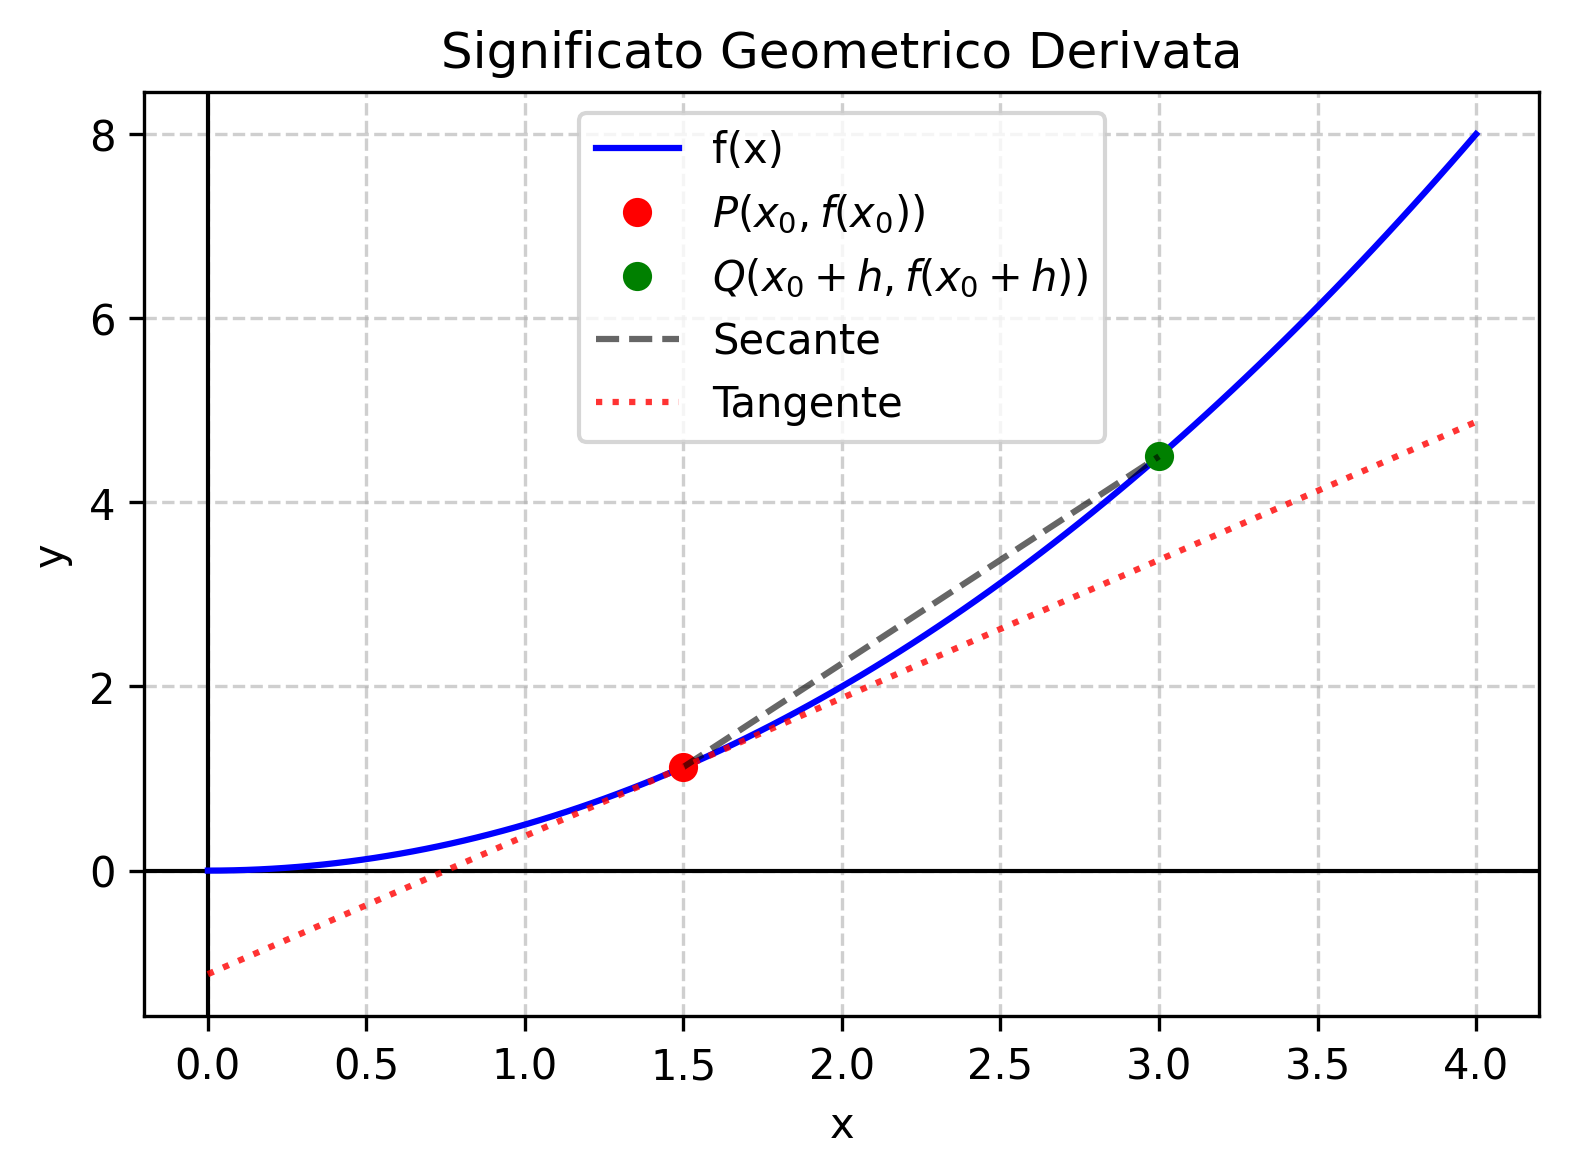
\includegraphics[width=0.7\textwidth]{img/rapporto_incrementale.png}
    \end{center}
    Prendiamo la secante passante per i punti \(P\) e \(Q\) e avviciniamoli (facendo tendere \(h \to 0\)).
    L'equazione della secante è:
    \[s: y=f(x_{0})+m(x-x_{0}) \quad \text{con } m=\frac{\Delta f}{\Delta x}\]
    
    Passaggio al limite:
    \begin{align*}
    &s: y=f(x_{0})+\frac{f(x_{0}+h)-f(x_{0})}{h}(x-x_{0})\\
    &h\to 0 \implies \\
    &\frac{f(x_{0}+h)-f(x_{0})}{h} \to l \\
    & s\to t:y=f(x_{0})+l(x-x_{0})
    \end{align*}
}

\subsection{Definizione di Derivata}

\defn{Derivata}{
    Si chiama \textbf{derivata} di \(f\) in \(x_{0}\) il seguente limite, se esiste finito:
    \[\lim_{ h \to 0 } \frac{f(x_{0}+h)-f(x_{0})}{h}=l\in \mathbb{R}\]
    Tale limite si denota con uno dei seguenti simboli:
    \begin{itemize}
        \item \(f'(x_{0})\)
        \item \(\frac{d}{dx}f(x_{0})\)
        \item \(Df(x_{0})\)
    \end{itemize}
    Se \(f\) ha derivata in \(x_{0}\), si dice \textbf{derivabile} in \(x_{0}\).
    Se \(f\) è derivabile \(\forall x_{0} \in ]a,b[\) diremo che \(f\) è derivabile.
}

\defn{Retta Tangente}{
    Se \(f\) è derivabile in \(x_{0}\), la retta
    \[y=f(x_{0})+f'(x_{0})(x-x_{0})\]
    prende il nome di \textbf{retta tangente} al grafico di \(f\) nel punto \((x_{0},f(x_{0}))\) e \(f'(x_{0})\) è il suo coefficiente angolare.
    
    Posso anche scrivere la derivata nella forma alternativa:
    \[f'(x_{0})=\lim_{ h \to 0 } \frac{f(\overbrace{x_{0}+h}^{x})-f(x_{0})}{h}=\lim_{ x \to x_{0} } \frac{f(x)-f(x_{0})}{x-x_{0}}\]
}

\subsection{Derivata Destra e Sinistra}

Se consideriamo una funzione definita su un intervallo chiuso o se vogliamo studiare la derivabilità agli estremi \(x_{0}=a\) o \(x_{0}=b\), definiamo:

\defn{Derivata Destra e Sinistra}{
    \begin{itemize}
        \item Se \(\lim_{ x \to x_{0}^+ } \frac{f(x)-f(x_{0})}{x-x_{0}} = l_+ \in \mathbb{R}\), allora lo indichiamo con \(f'_{+}(x_{0})\) e si chiama \textbf{derivata destra} in \(x_{0}\).
        \item Se \(\lim_{ x \to x_{0}^- } \frac{f(x)-f(x_{0})}{x-x_{0}} = l_- \in \mathbb{R}\), allora lo indichiamo con \(f'_{-}(x_{0})\) e si chiama \textbf{derivata sinistra} in \(x_{0}\).
    \end{itemize}
}

\rmkb{
    \(f\) è derivabile in \(x_{0} \iff f'_{+}(x_{0})\) e \(f'_{-}(x_{0})\) esistono finiti e coincidono:
    \[f'(x_{0})=f'_{+}(x_{0})=f'_{-}(x_{0})\]
}



\section{Derivate delle Funzioni Elementari}

Di seguito analizziamo le derivate delle funzioni fondamentali, dimostrandone i risultati tramite la definizione di rapporto incrementale.

\begin{enumerate}
    \item \textbf{Derivata di una costante} \(c\):
    \[ Dc(x)=0 \; \forall x\in \mathbb{R} \]
    Infatti: \(\lim_{ x \to x_{0} } \frac{c-c}{x-x_{0}}=0\).
    \begin{center}
        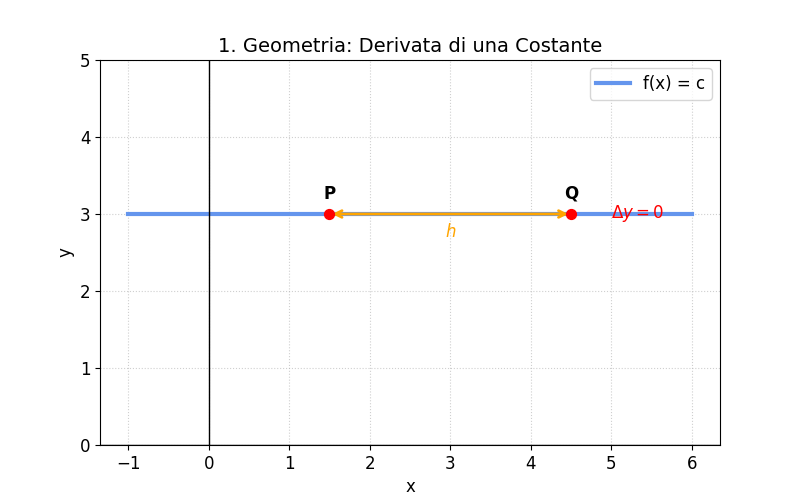
\includegraphics[width=0.6\textwidth]{img/der-di-costante.png}
    \end{center}

    \item \textbf{Derivata della retta} \(ax+b\):
    \[ D(ax+b)=\lim_{ h \to 0 } \frac{a(x+h)+b-ax-b}{h}=\lim_{ h \to 0 } \frac{ah}{h}=a \]
    \begin{center}
        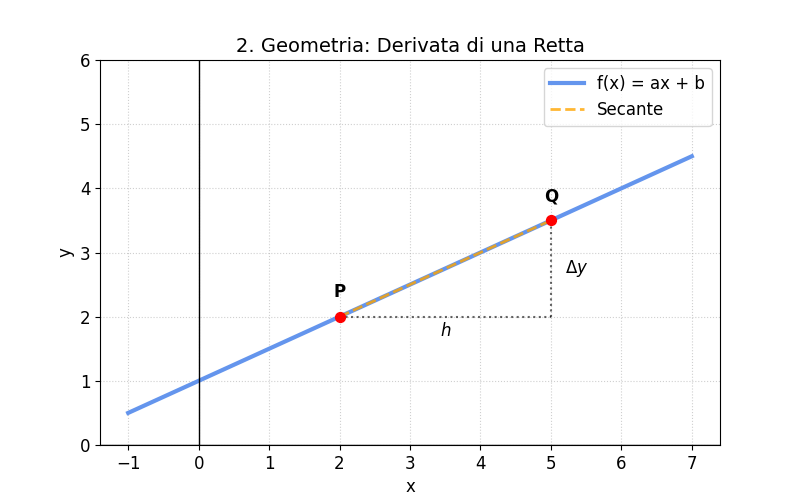
\includegraphics[width=0.6\textwidth]{img/der-di-retta.png}
    \end{center}
    \ex{
        \(D(x)=1\) \\
        \(D(-x)=-1\)
    }

    \item \textbf{Derivata del valore assoluto} \(|x|\):
    \[
    |x|=\begin{cases}
    x & x\geq 0 \\
    -x & x<0
    \end{cases} \implies
    D(|x|)=\begin{cases}
    1 & x>0 \\
    -1 & x<0 \\
    \not \exists & x=0
    \end{cases}
    \]
    Perché in \(x=0\):
    \[\lim_{ h \to 0 } \frac{|0+h|-|0|}{h}=\frac{|h|}{h}=\begin{cases} 1 & h \to 0^+ \\ -1 & h \to 0^- \end{cases} \implies \not \exists\]

    \item \textbf{Derivata della potenza} \(x^\alpha\):
    \[ D(x^\alpha)=\alpha x^{\alpha-1} \]
    \pf{
        \begin{align*}
        & \lim_{ h \to 0 } \frac{f(x+h)-f(x)}{h}=\lim_{ h \to 0 } \frac{(x+h)^\alpha-x^\alpha}{h}= \left[\frac{0}{0}\right] \\
        & = \lim_{ h \to 0 } \frac{x^\alpha \left( \left( 1+\frac{h}{x} \right)^\alpha-1 \right)}{h}=\lim_{ h \to 0 } \frac{x^{\alpha-1}\left( \left( 1+\frac{h}{x} \right)^\alpha-1 \right)}{\frac{h}{x}}=\alpha x^{\alpha-1}
        \end{align*}
    }
    \ex{
        \begin{itemize}
            \item \(D(\sqrt{ x }) = D(x^{1/2}) = \frac{1}{2}x^{\frac{1}{2} -1}=\frac{1}{2\sqrt{ x }}\)
            \item \(D(x^3)=3x^2\)
        \end{itemize}
    }

    \item \textbf{Derivata dell'esponenziale} \(a^x\):
    \[ D(a^x) = a^x \log a \]
    \pf{
        \[\lim_{ h \to 0 } \frac{a^{x+h}-a^x}{h}=\lim_{ h \to 0 } \frac{a^x(a^h-1)}{h} = a^x\log a\]
    }

    \item \textbf{Derivata di} \(e^x\):
    \[ D(e^x)=e^x \]
    (Segue dalla (5) ponendo \(a=e\), dato che \(\log e = 1\)).

    \item \textbf{Derivata del Seno}:
    \[ D(\sin x)=\cos x \]
    \pf{
        \begin{align*}
        &\lim_{ h \to 0 } \frac{\sin(x+h)-\sin x}{h}= \lim_{ h \to 0 } \frac{\sin x\cos h + \cos x \sin h - \sin x}{h}=\\
        & = \lim_{ h \to 0 } \left[ \sin x \left( \frac{\cos h-1}{h} \right) + \cos x\left( \frac{\sin h}{h} \right) \right] = \sin x \cdot 0 + \cos x \cdot 1 = \cos x
        \end{align*}
    }

    \item \textbf{Derivata del Coseno}:
    \[ D(\cos x)=-\sin x \]
    \pf{
        \begin{align*}
        &\lim_{ h \to 0 } \frac{\cos(x+h)-\cos x}{h}=\lim_{ h \to 0 } \frac{\cos x \cos h - \sin x \sin h - \cos x}{h}=\\
        & = \lim_{ h \to 0 } \left[ \cos x\frac{(\cos h-1)}{h} - \sin x \cdot \frac{\sin h}{h} \right] = -\sin x
        \end{align*}
    }

    \item \textbf{Derivata del Logaritmo} \(\log_a x\):
    \[ D(\log_{a}x) = \frac{1}{x \log a} \]
    \pf{
        \[\lim_{ h \to 0 } \frac{\log_{a}(x+h)-\log_{a}(x)}{h}=\lim_{ h \to 0 } \frac{1}{h} \log_{a}\left( 1+ \frac{h}{x} \right) = \lim_{ h \to 0 } \frac{1}{x} \frac{\log_{a}(1+t)}{t} = \frac{1}{x\log a}\]
        (dove \(t = h/x \to 0\)).
    }

    \item \textbf{Derivata di} \(\log x\) (base \(e\)):
    \[ D(\log x)=\frac{1}{x} \]

\end{enumerate}

\section{Algebra delle Derivate}

\thm{Operazioni con le Derivate}{
    Siano \(f, g\) definite in \(]a,b[\) e derivabili in \(x_{0}\). Allora anche \(c \cdot f\), \(f\pm g\), \(f \cdot g\) e \(\frac{f}{g}\) (se \(g(x_0)\neq 0\)) sono derivabili in \(x_{0}\) e risulta:
    \begin{enumerate}
        \item \(D(cf(x_{0}))=cDf(x_{0})\)
        \item \(D(f\pm g)(x_0)=Df(x_{0})\pm Dg(x_{0})\)
        \item \(D(fg)(x_{0})=Df(x_{0})g(x_{0})+f(x_{0})Dg(x_{0})\)
        \item \(D\left( \frac{f}{g} \right)(x_{0})=\frac{Df(x_{0})g(x_{0})-f(x_{0})Dg(x_{0})}{g^2(x_{0})}\)
    \end{enumerate}
    Le proprietà (1) e (2) indicano che la derivata è un \textbf{operatore lineare}.
}

\pf{
    \textbf{Dimostrazione (2) - Somma:}
    \[\lim_{ h \to 0 } \frac{f(x_{0}+h)+g(x_{0}+h)-(f(x_{0})+g(x_{0}))}{h}= \]
    \[=\lim_{ h \to 0 } \left[ \frac{f(x_0+h)-f(x_0)}{h} + \frac{g(x_0+h)-g(x_0)}{h} \right]=\]
    \[= f'(x_{0})+g'(x_{0})\]
}

Per dimostrare rigorosamente la regola del prodotto, necessitiamo prima di un legame tra derivabilità e continuità.

\thm{Relazione Derivabilità-Continuità}{
    Se \(g\) è definita in \(]a,b[\) ed è derivabile in \(x_{0} \implies g\) è continua in \(x_{0}\).
    
    Il viceversa non vale: \(\centernot \impliedby\). Esempio: \(|x|\) è continua in \(x=0\) ma non derivabile.
}

\pf{
    Per dimostrare che \(g\) è continua in \(x_{0}\) devo dimostrare che \(\lim_{ x \to x_{0} } g(x)=g(x_{0})\), ovvero che \(\lim_{ x \to x_{0} } (g(x)-g(x_{0}))=0\).
    Possiamo scrivere:
    \[\lim_{ x \to x_{0} } (g(x)-g(x_{0})) = \lim_{ x \to x_{0} } \frac{g(x)-g(x_{0})}{x-x_{0}}(x-x_{0}) = g'(x_0) \cdot 0 = 0\]
}

\pf{
    \textbf{Dimostrazione (3) - Prodotto:}
    \begin{align*}
    &\lim_{ x \to x_{0} } \frac{f(x)g(x)-f(x_{0})g(x_{0})}{x-x_{0}} \\ 
    &= \lim_{ x \to x_{0} } \frac{f(x)g(x) - f(x_0)g(x) + f(x_0)g(x) - f(x_0)g(x_0)}{x-x_{0}} \\ 
    &= \lim_{ x \to x_{0} } \left( g(x) \frac{f(x)-f(x_0)}{x-x_0} + f(x_0) \frac{g(x)-g(x_0)}{x-x_0} \right) \\ 
    &= g(x_0)f'(x_0) + f(x_0)g'(x_0) 
    \end{align*}
    (Qui abbiamo usato il fatto che \(\lim_{x \to x_0} g(x) = g(x_0)\) perché \(g\) è derivabile e quindi continua).
}

\ex{
    \textbf{Derivata della Tangente}:
    \begin{align*}
    & D(\tan x) = D\left(\frac{\sin x}{\cos x} \right)=\frac{\cos x \cdot \cos x - \sin x (-\sin x)}{\cos^2 x} = \\
    &\frac{\cos^2 x + \sin^2 x}{\cos^2 x} = \\
    & \frac{1}{\cos^{2}x} = 1+\tan^2 x
    \end{align*}
}

\section{Teoremi Fondamentali del Calcolo}

\thm{Derivazione delle Funzioni Composte (Chain Rule)}{
    Siano \(g,f\) tali che sia definita la funzione composta \(f(g(x))\).
    Sia \(x_{0}\) tale che \(g\) è derivabile in \(x_{0}\) e \(f\) è derivabile in \(g(x_{0})\).
    Allora \(f \circ g\) è derivabile in \(x_{0}\) e si ha:
    \[D(f \circ g)(x)=(f \circ g)'(x_{0})=f'(g(x_{0}))\cdot g'(x_{0})\]
}

\pf{
    Definiamo la funzione ausiliaria \(H(y)\):
    \[H(y)=\begin{cases}
    \frac{f(y)-f(y_{0})}{y-y_{0}} & y\ne y_0\\
    f'(y_{0}) & y=y_{0}
    \end{cases}\]
    dove \(y_0 = g(x_0)\). \(H\) è continua in \(y_{0}\).
    Possiamo scrivere il rapporto incrementale come:
    \[\frac{f(g(x))-f(g(x_{0}))}{x-x_{0}} = H(g(x))\frac{g(x)-g(x_{0})}{x-x_{0}}\]
    Passando al limite per \(x \to x_0\):
    \[\lim_{ x \to x_{0} } H(g(x))\frac{g(x)-g(x_{0})}{x-x_{0}} = H(g(x_0)) \cdot g'(x_0) = f'(g(x_{0}))\cdot g'(x_{0})\]
}

\thm{Derivata della Funzione Inversa}{
    Sia \(f\) strettamente monotona e continua in \(]a,b[\).
    Sia \(f\) derivabile in \(x_{0}\in]a,b[\) e \(f'(x_{0})\neq 0\).
    Allora la funzione inversa \(f^{-1}\) è derivabile in \(y_{0}=f(x_{0})\) e risulta:
    \[(f^{-1})'(y_{0})=\frac{1}{f'(f^{-1}(y_{0}))}=\frac{1}{f'(x_{0})}\]
}

\begin{center}
    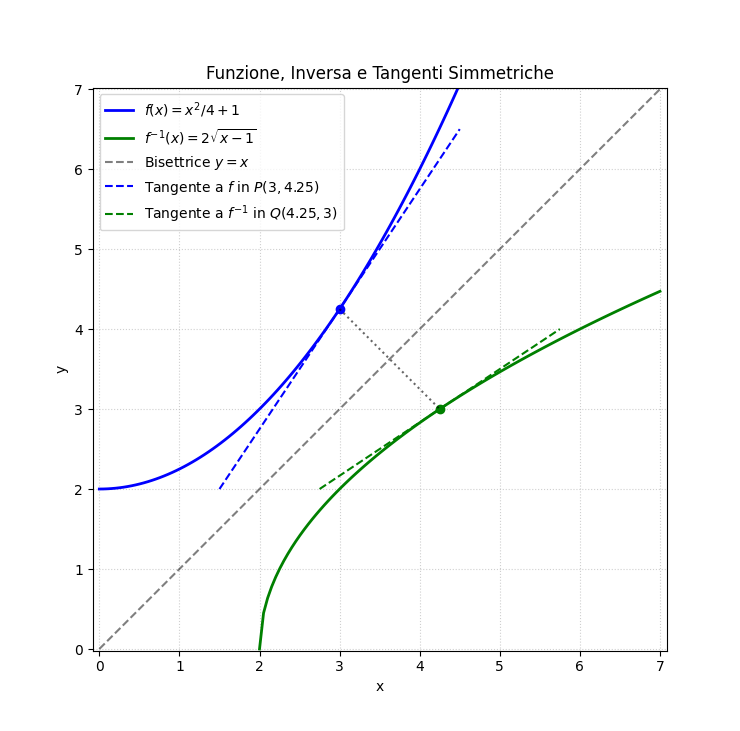
\includegraphics[width=0.6\textwidth]{img/derivata_funzione_inversa.png}
\end{center}

\rmkb{
    Interpretazione geometrica: Se la retta tangente in \(P(x_0, y_0)\) forma un angolo \(\alpha\) con l'asse \(x\), allora \(f'(x_0) = \tan \alpha\). Rispetto all'asse \(y\) (scambiando gli assi per l'inversa), l'angolo è \(\beta = \frac{\pi}{2} - \alpha\).
    \[(f^{-1})'(y_{0})=\tan \beta = \tan\left( \frac{\pi}{2} -\alpha \right)=\frac{1}{\tan \alpha}=\frac{1}{f'(x_{0})}\]
}

\subsection{Derivate delle Funzioni Inverse Trigonometriche}

\ex{
    \textbf{Arcoseno}:
    \[D(\arcsin x)=\frac{1}{D(\sin y)}\bigg|_{y=\arcsin x}=\frac{1}{\cos y}\]
    Poiché \(y \in [-\frac{\pi}{2}, \frac{\pi}{2}]\), \(\cos y \ge 0\), quindi \(\cos y = \sqrt{1-\sin^2 y}\).
    \[= \frac{1}{\sqrt{ 1-\sin^2 (\arcsin x) }} = \frac{1}{\sqrt{ 1-x^2 }}\]
}

\ex{
    \textbf{Arcocoseno}:
    \[D(\arccos x) = \frac{1}{D(\cos y)}\bigg|_{y=\arccos x} = \frac{1}{-\sin y}\]
    Poiché \(y \in [0, \pi]\), \(\sin y \ge 0\), quindi \(\sin y = \sqrt{1-\cos^2 y}\).
    \[= -\frac{1}{\sqrt{1-x^2}}\]
}

\ex{
    \textbf{Arcotangente}:
    \[D(\arctan x) = \frac{1}{D(\tan y)}\bigg|_{y=\arctan x} = \cos^2 y = \frac{1}{1+\tan^2 y} = \frac{1}{1+x^2}\]
}


\section{Punti di non derivabilità}\label{punti-di-non-derivabilituxe0}

% Utilizzo dell'ambiente \defn definito in theorems.tex
% Argomento 1: Titolo (opzionale o desunto dal testo)
% Argomento 2: Contenuto
\defn{\(f\) non derivabile}{
    Se \(f\) non è derivabile in \(x_{0}\):
    \[
    \lim_{ x \to x_{0} } \frac{f(x)-f(x_{0})}{x-x_{0}}=\begin{cases}
    \not \exists \\ 
    \infty
    \end{cases}
    \]
}

\begin{enumerate}
    \item \(f'_{+}(x_{0})\) e \(f'_{-}(x_{0}) \exists\) finite ma:
    \[f'_{+}(x_{0})\neq f'_{-}(x_{0})\] 
    In questo caso si chiama \textbf{punto angoloso}. Assumiamo che \(x_{0}\) è un punto angoloso anche quando una delle due derivate \(f'_{+}(x_{0})\) e \(f'_{-}(x_{0})\) è finita, mentre l'altra è \(\pm \infty\).
\end{enumerate}


\ex{
    \[
    f(x)=\begin{cases}
    \sqrt{ x } & x\geq{0} \\
    1- e^{-x/2} & x<0 
    \end{cases}
    \implies f\text{ è continua in } \mathbb{R}
    \]
    \[f'_{+}(0)= +\infty \qquad f'_{-}(0)=-\frac{1}{2}\]
    \begin{center}
    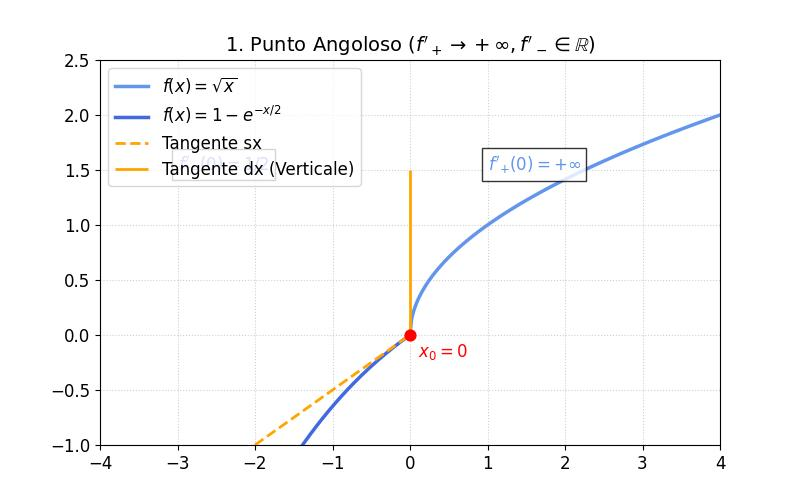
\includegraphics[width=0.7\textwidth]{img/punto_angoloso.png}
    \end{center}
}

\begin{enumerate}
    \setcounter{enumi}{1}
    \item Se \(f'_{+}(x_{0})=+\infty\) e \(f'_{-}(x_{0})=-\infty\) o viceversa, \(x_{0}\) si dice \textbf{cuspide}.
\end{enumerate}

\ex{
    \[ f(x)=\sqrt{ |x| } \]
    \begin{center}
    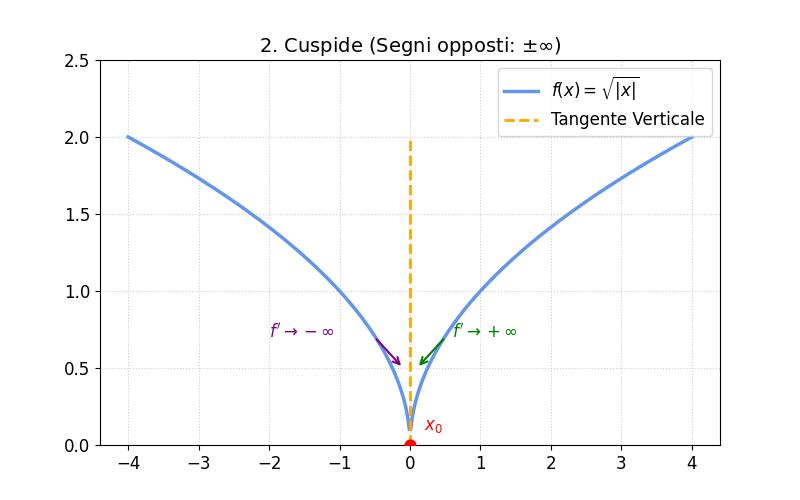
\includegraphics[width=0.7\textwidth]{img/cuspide.png}
    \end{center}
}

\begin{enumerate}
    \setcounter{enumi}{2}
    \item Se \(f'_{+}(x_{0})=f'_{-}(x_{0})=\pm \infty\) (\(\infty\) ma con lo stesso segno), \(x_{0}\) è \textbf{a tangente verticale.}
\end{enumerate}

\ex{
    \[ y=\sqrt[3]{x} \]
    \begin{center}
    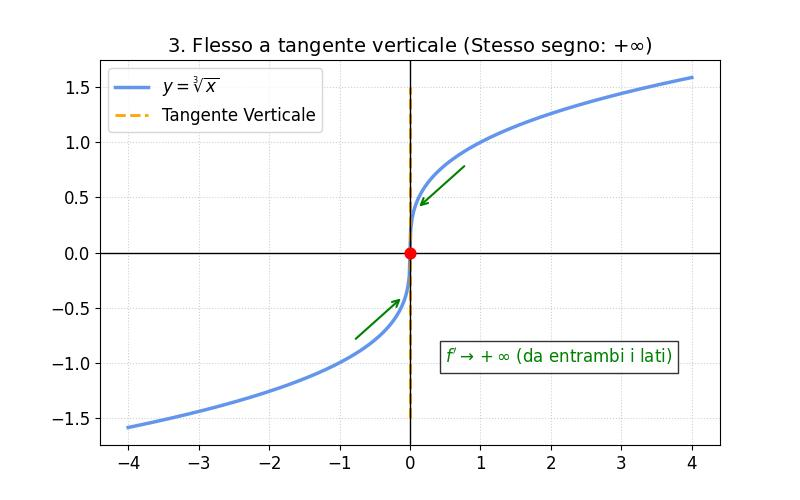
\includegraphics[width=0.7\textwidth]{img/flesso-tan-ver.png}
    \end{center}
}

Tutti gli altri sono punti di non derivabilità.

\rmkb{
    Le funzioni con derivata limitata sono sempre Lipschitziane.
}



\section{Estremi relativi}

\defn{Min relativo e punto di Min relativo}{
    Sia $f:A \subseteq \mathbb{R}\to \mathbb{R}, \quad A\neq \emptyset$.
    Un punto $x_{0}\in A$ si dice punto di minimo relativo per $f$ se $\exists I_{\delta}(x_{0})=]x_{0}-\delta,x_{0}+\delta[$ tale che:
    \[
    f(x)\geq f(x_{0}) \; \forall x \in A \cap I_{\delta}(x_{0})
    \]
    e $f(x_{0})$ si dice minimo relativo.
}

\defn{Max relativo e punto di Max relativo}{
    Se $\exists I_{\delta}(x_{0})=]x_{0}-\delta,x_{0}+\delta[$ tale che:
    \[
    f(x_{0})\geq f(x) \; \forall x \in A \cap I_{\delta}(x_{0})
    \]
    allora $x_{0}$ si dirà punto di massimo relativo e $f(x_{0})$ massimo relativo.
}

\ex{
    \begin{center}
        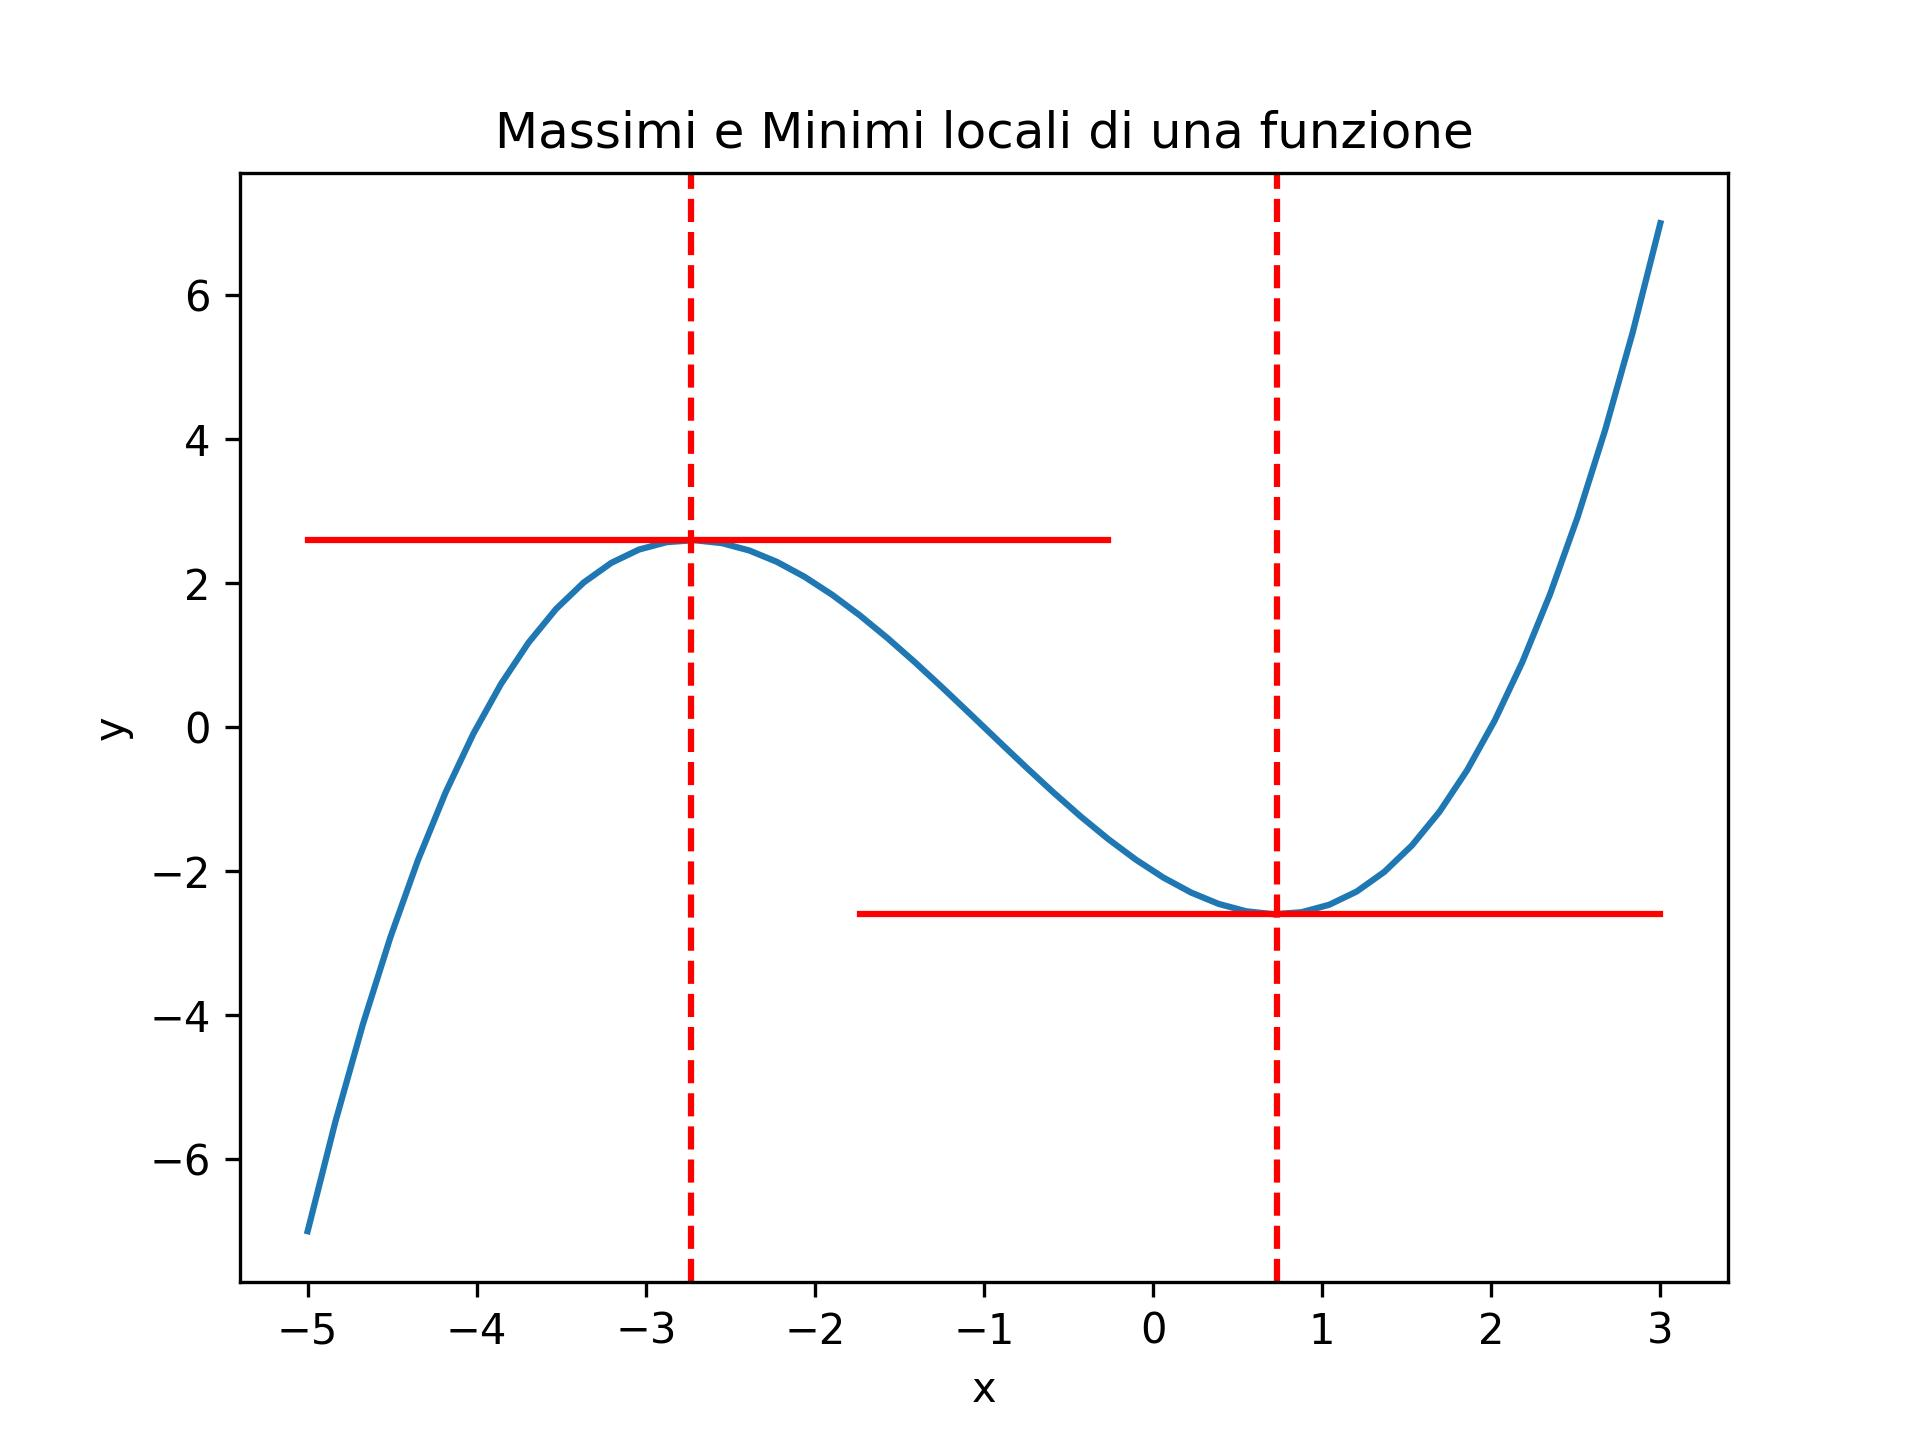
\includegraphics[width=0.7\textwidth]{img/estremi-relativi.jpg}
    \end{center}
}

\rmkb{NON SONO UNICI}

\subsection{Teorema di Fermat}

\thm{Teorema di Fermat (condizione necessaria del $1^{\circ}$ ordine)}{
    Sia $f:[a,b]\to \mathbb{R}$ e sia $x_{0}\in]a,b[$ un punto in cui $f$ è derivabile ed in un punto di estremo relativo.
    Allora ($\implies$):
    \[
    f'(x_{0})=0
    \]
}

\ex{
    \begin{center}
        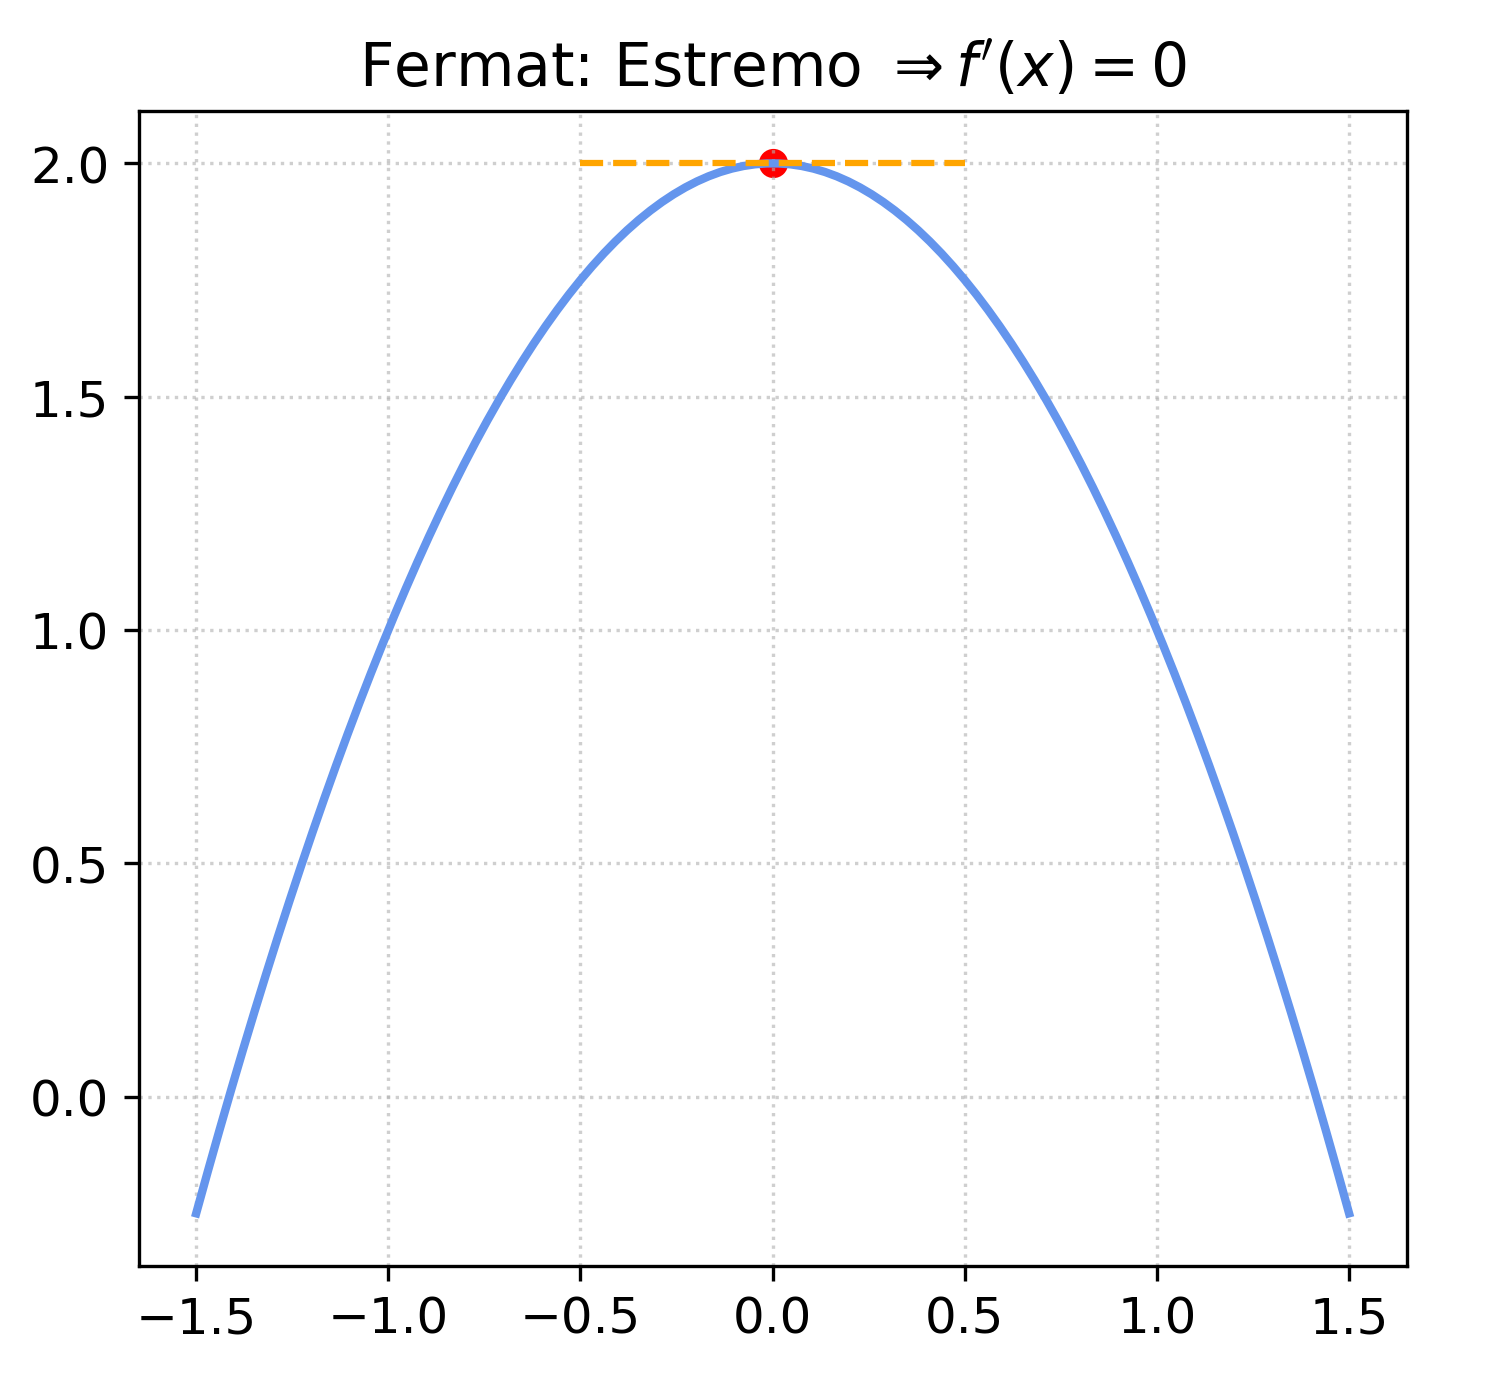
\includegraphics[width=0.7\textwidth]{img/teorema_fermat_es.png}
    \end{center}
}

\ex{
    Vale $\impliedby$? NO
    \begin{itemize}
        \item $\centernot \impliedby$
    \end{itemize}
    $f(x)=x^3 \quad f'(x)=3x^2$
    \begin{center}
        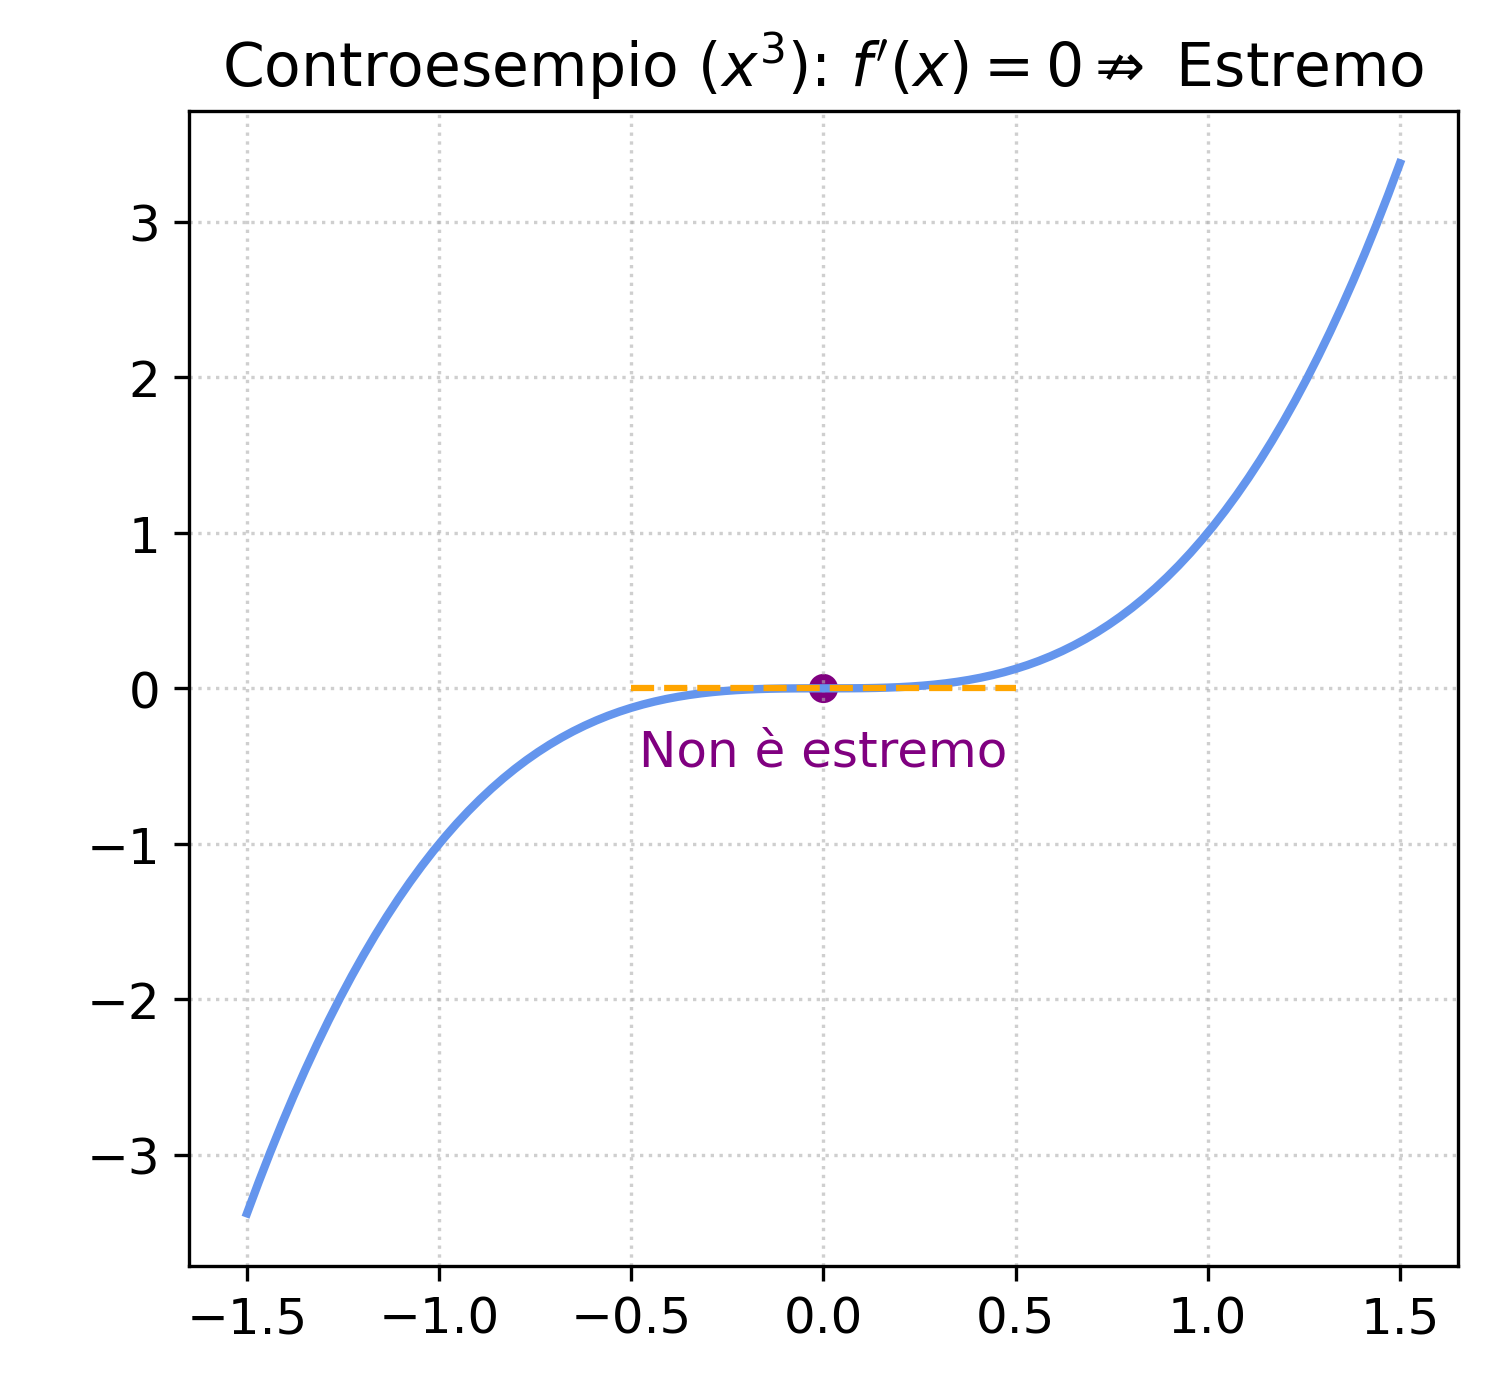
\includegraphics[width=0.7\textwidth]{img/teorema_fermat_controes.png}
    \end{center}
}

\pf{
    Supponiamo per semplicità che $x_{0}$ sia punto di minimo relativo, $\exists I_{\delta}(x_{0}):$
    \[
    f(x_{0})\leq f(x) \; \forall x \in [a,b] \cap I_{\delta}(x_{0})
    \]
    Essendo $f$ derivabile in $x_{0}$ allora:
    \begin{align*}
    \exists \text{ finito } &\lim_{ x \to x_{0} } \frac{f(x)-f(x_{0})}{x-x_{0}}=f'(x_{0}) \textcolor{orange}{=0}\\
    & =\lim_{ x \to x_{0}^- } \frac{f(x)-f(x_{0})}{x-x_{0}}=f'_{-}(x_{0}) \textcolor{orange}{\leq0}\\
    & =\lim_{ x \to x_{0}^+ } \frac{f(x)-f(x_{0})}{x-x_{0}}=f'_{+}(x_{0}) \textcolor{orange}{\geq0} 
    \end{align*}
    Il Numeratore è sempre positivo perchè nel limite, $x$ entra in $I_{\delta}(x_{0})$.
    Il segno del Denominatore dipende dal lato da cui avvicino, allora per avere l'uguaglianza, devono essere tutte (le derivate) = 0.
}

\defn{Definizione}{
    Sia $f$ derivabile in $]a,b[$, i punti $x: f'(x) = 0$.
    Si dicono \textbf{punti critici o stazionari}.
}

\subsubsection*{Esempio di esercizio}

\ex{
    \[ f(x)=2-\log(1+|x|) \qquad x\in[-1,3] \]
    Uso Weierstrass: $\exists$ estremi assoluti.
    Lista:
    \begin{enumerate}
        \item "Punti di Fermat"
        \item Punti di non Derivabilità
        \item Estremi
    \end{enumerate}
    
    \[
    f(x)= \begin{dcases}
    2-\log(1+x) \quad x\in[0,3] \\
    2-\log(1-x) \quad x \in[-1,0]
    \end{dcases}
    \]
    \[
    f'(x)= \begin{dcases}
    -\frac{1}{(1+x)} \quad x\in]0,3] \\
    \not \exists  \quad \qquad \qquad x=0\\
    \frac{1}{(1+x)} \quad x \in[-1,0[
    \end{dcases}\implies\text{Punto angoloso}
    \]
    \[ f(0)=2=M \qquad f(3)=2-\log_{4}=m \qquad f(-1)=2-\log_{2} \]
    
    Svolgimento lista:
    \begin{enumerate}
        \item $\to\varnothing$
        \item $\to x=0$
        \item $\to x=-1 \quad x=3$
    \end{enumerate}
}

\subsection{Teorema di Rolle}

\thm{Teorema di Rolle}{
    \begin{itemize}
        \item Sia $f:[a,b]\to \mathbb{R}$ continua
        \item Sia $f$ derivabile in $]a,b[$
        \item Se $f(a)=f(b)$ allora $\exists c \in ]a,b[:f'(c)=0$
    \end{itemize}
}

\ex{
    \begin{center}
        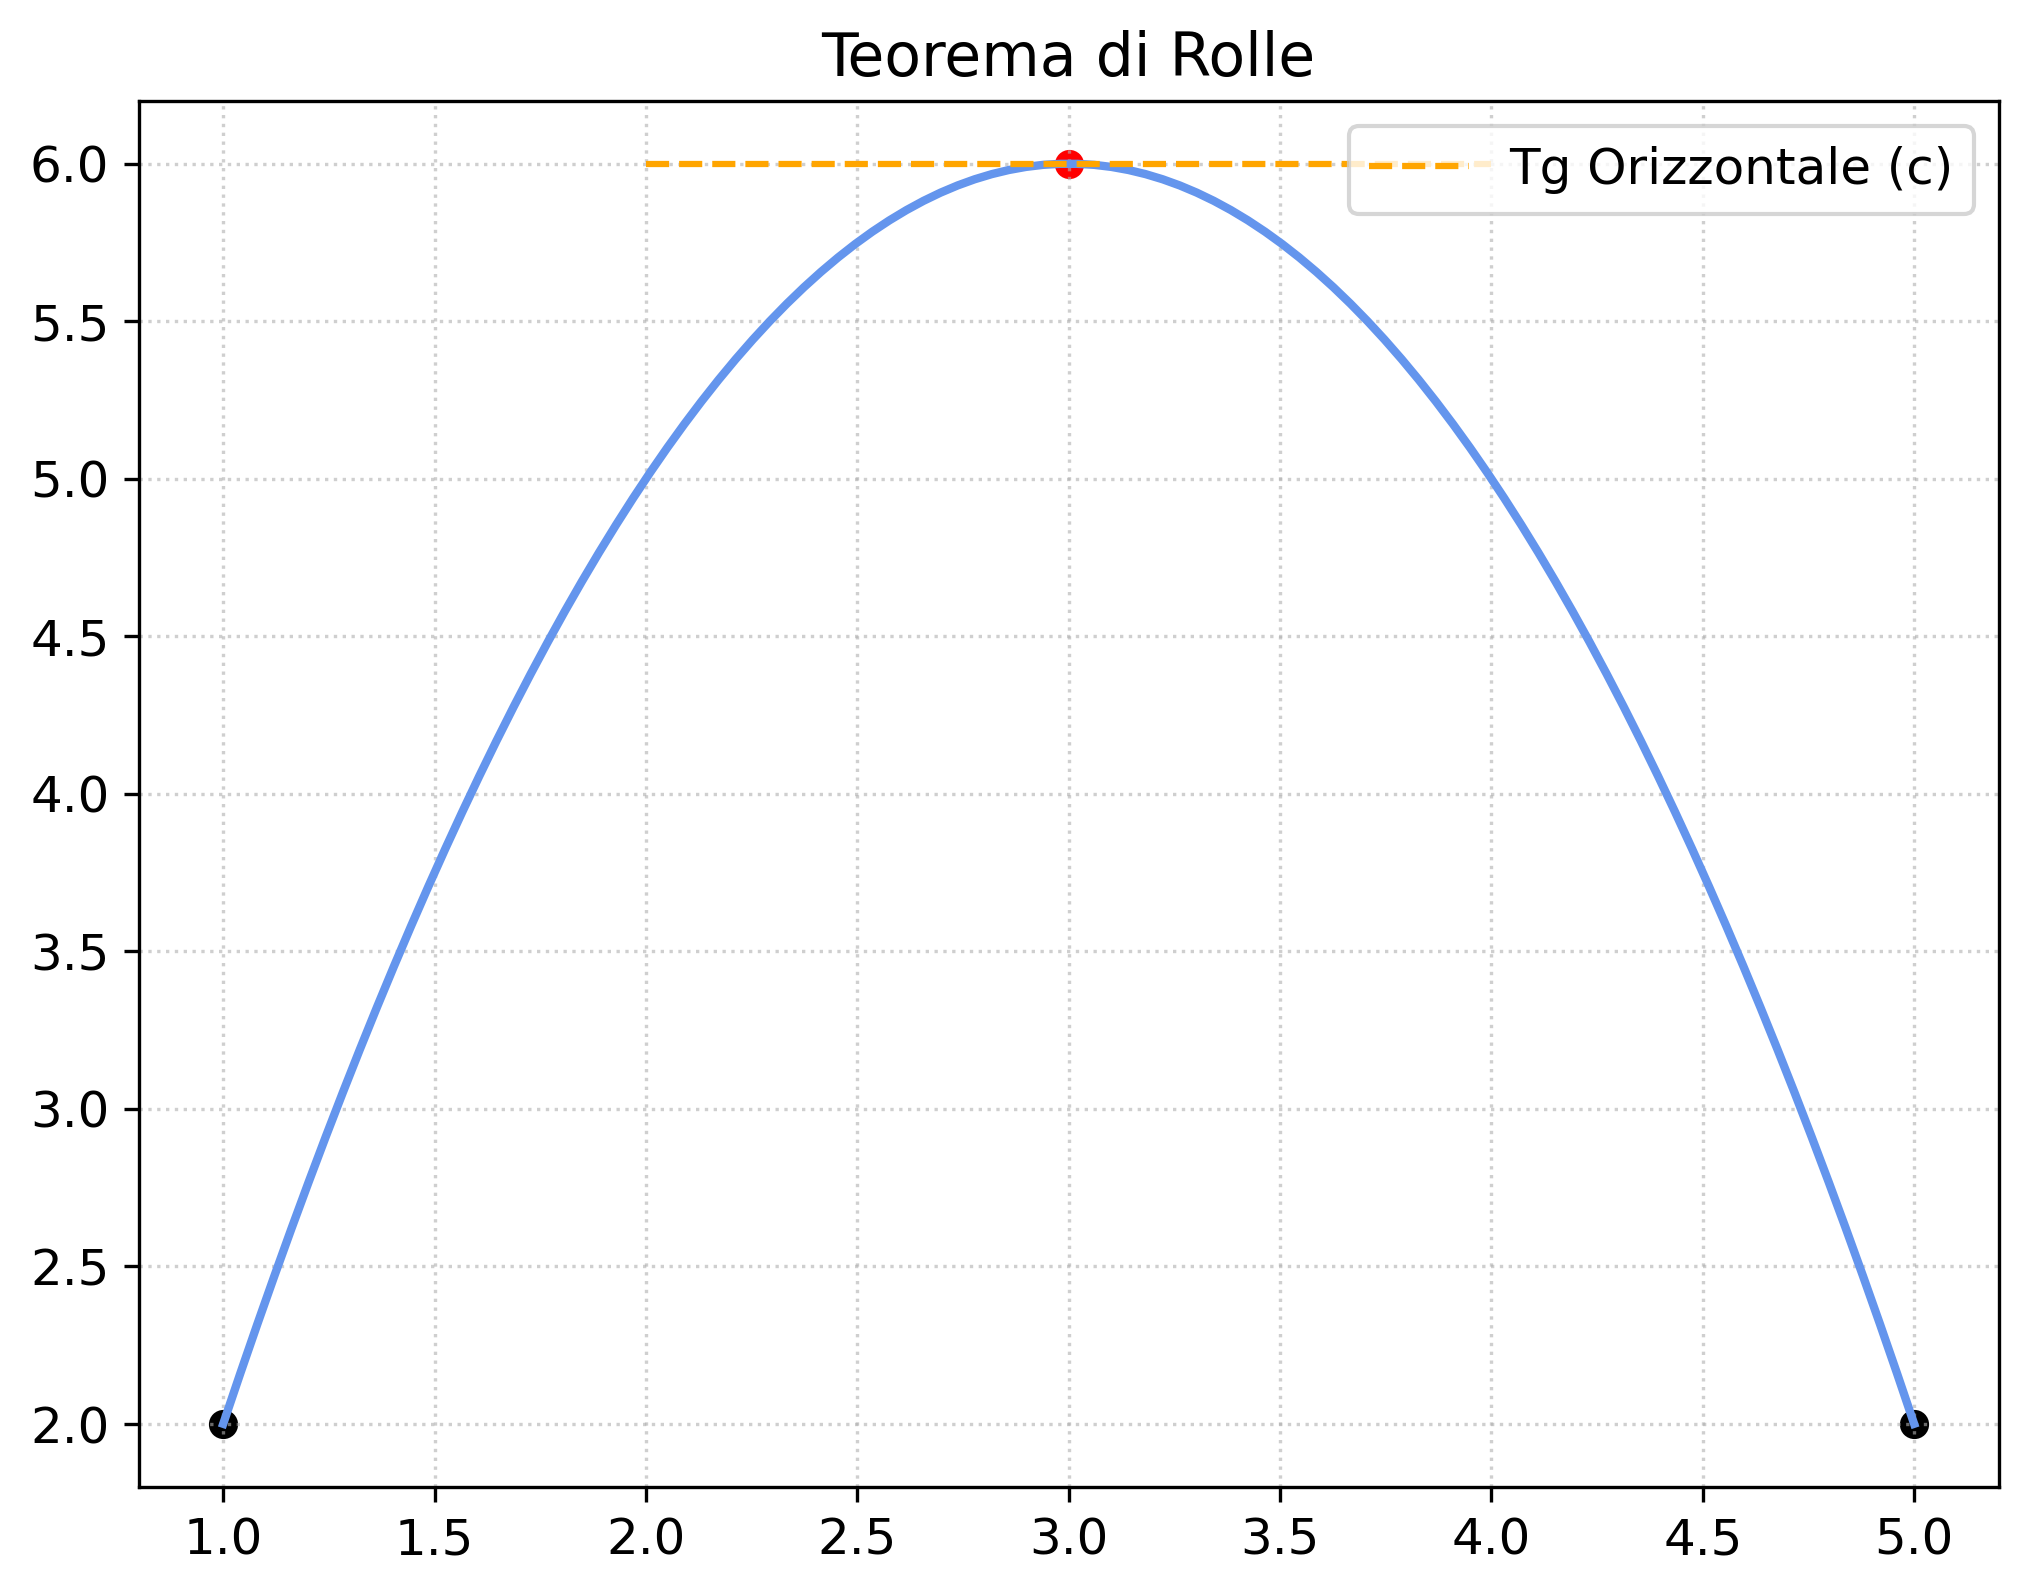
\includegraphics[width=0.7\textwidth]{img/teorema_rolle.png}
    \end{center}
}

\ex{
    Non posso rimuovere la prima ipotesi
    \begin{center}
        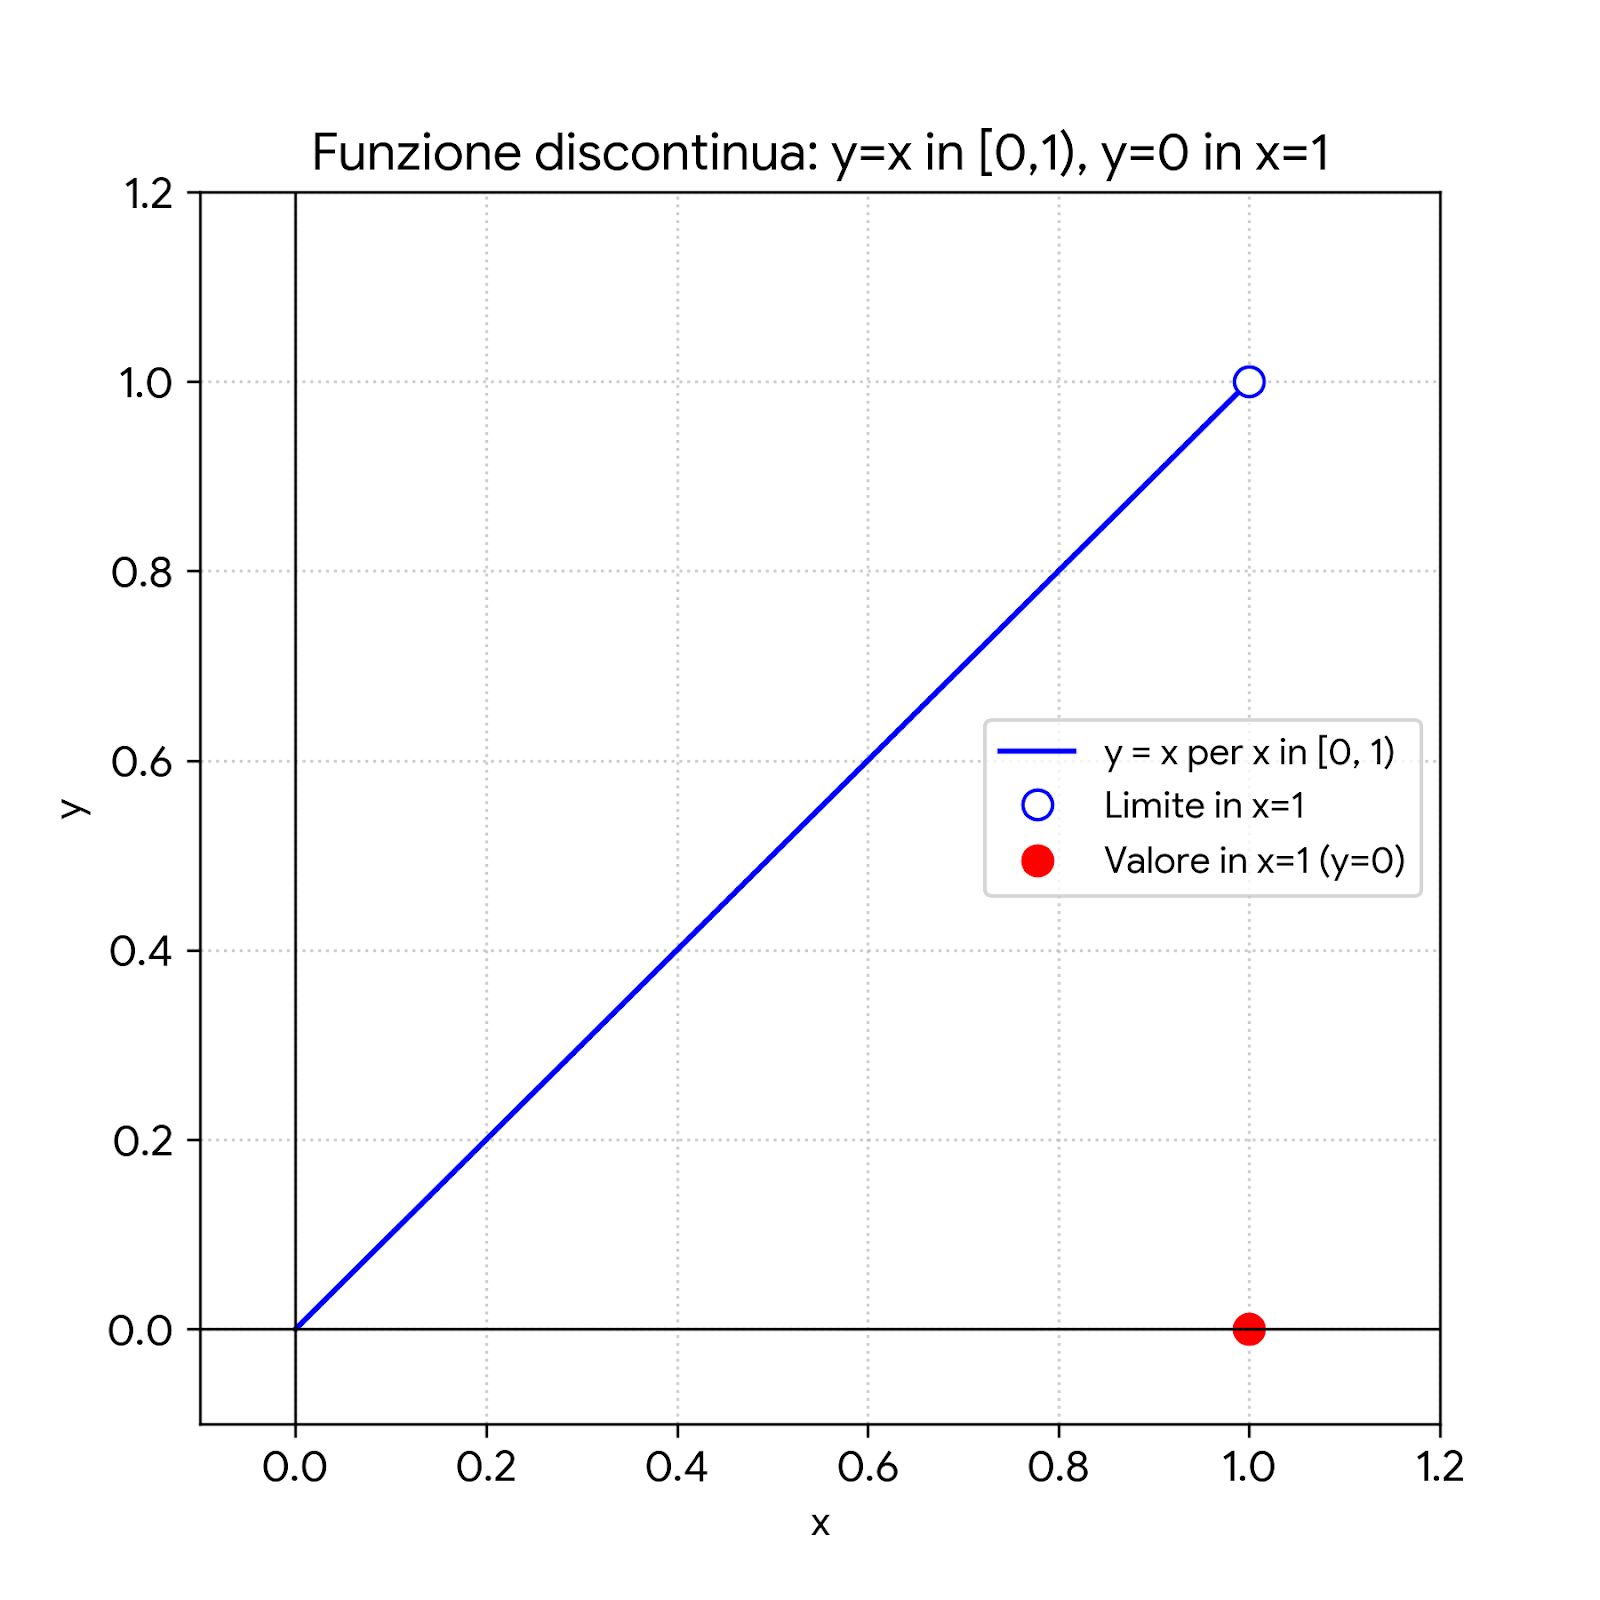
\includegraphics[width=0.7\textwidth]{img/percentuale-2.png}
    \end{center}
}

\pf{
    $\exists m = f(x_{m})$ e $M=f(x_{M})$ per Weierstrass con $x_{m}\in[a,b], x_{M}\in[a,b]$.
    Ovviamente $x_{m}\neq x_{M}$ altrimenti $f$ è costante:
    $m=M$ e in tal caso $\forall c \in [a,b] \implies f'(c)=0$.
    Ma se $x_{m}\neq x_{M}$ allora essendo per hp $f(a)=f(b)$ almeno uno dei 2 punti tra $x_{m}$ e $x_{M}$ deve essere interno ad $]a,b[$.
    Supponiamo che sia $x_{m}\in]a,b[\implies$ per Fermat $f'(x_{m})=0$.
}

\subsection{Teorema di Lagrange}

\thm{Teorema di Lagrange}{
    \begin{itemize}
        \item Sia $f:[a,b]\to \mathbb{R}$ continua 
        \item Sia $f$ derivabile in $]a,b[$
        \item Allora $\exists c \in]a,b[:$
        \[ m=f'(c)=\frac{f(b)-f(a)}{b-a} \]
    \end{itemize}
}

\ex{
    \begin{center}
        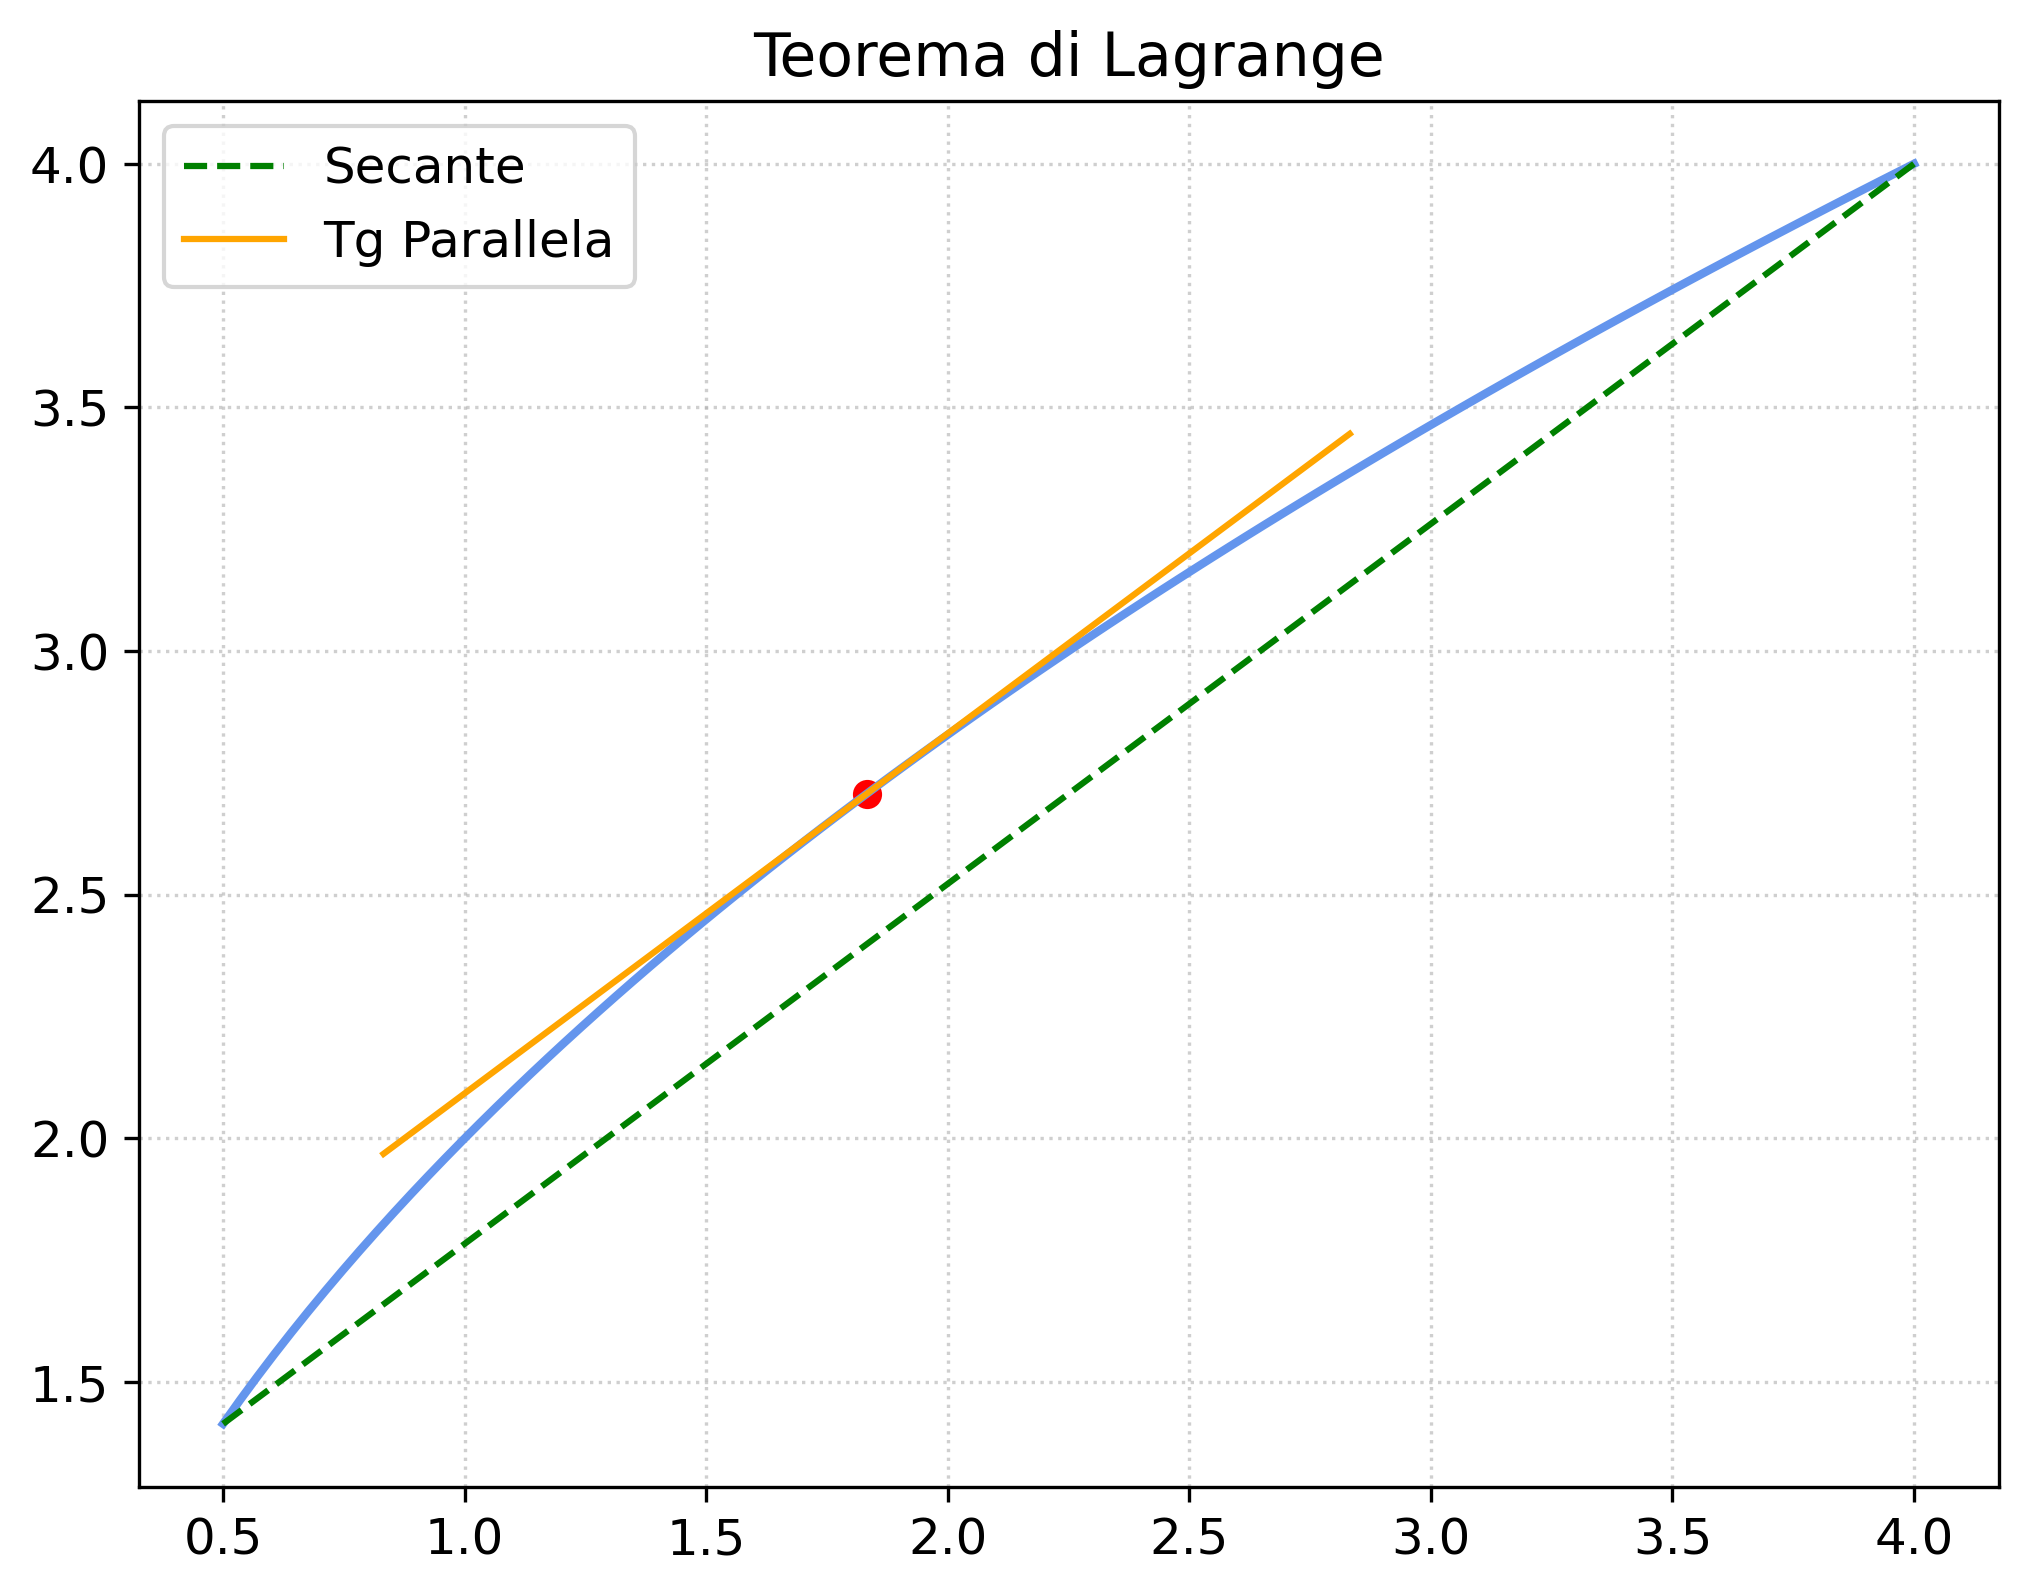
\includegraphics[width=0.7\textwidth]{img/teorema_lagrange.png}
    \end{center}
}

\pf{
    Consideriamo
    \[ g(x)=f(x)-\frac{f(b)-f(a)}{b-a}(x-a) \]
    \begin{itemize}
        \item $g$ è continua in $[a,b]$ (perchè è somma di funzioni continue)
        \item $g$ è derivabile in $]a,b[$
        \item $\begin{dcases}g(a)=f(a) \\ g(b)=f(a)\end{dcases}\implies \exists c \in]a,b[: g'(c)=0\implies$
    \end{itemize}
    \[ \implies f'(c)-\frac{f(b)-f(a)}{b-a}=0 \]
}

\subsubsection{Conseguenze del Teorema di Lagrange}

\thm{Teorema di Caratterizzazione delle funzioni costanti}{
    \begin{itemize}
        \item Sia $f$ continua in $[a,b]$
        \item Sia $f$ derivabile in $]a,b[$
    \end{itemize}
    \[ f \text{ è costante }\iff f'(x)=0 \implies \forall x \in ]a,b[ \]
}

\pf{
    \begin{itemize}
        \item ($\implies$) Ovvia
        \item ($\impliedby$) ($f'=0 \; \forall x \in]a,b[\implies f(x)\text{ costante}$)
    \end{itemize}
    Prendiamo $x_{0}\in]a,b[$ e $x\neq x_{0}$.
    Dimostriamo che $f(x)=f(x_{0})$.
    Applico Lagrange in $]x,x_{0}[$ o $]x_{0},x[$ a seconda di come si confrontano.
    Assumiamo che sia $]x,x_{0}[$ allora $\exists c \in ]x,x_{0}[:$
    \[ \frac{f(x)-f(x_{0})}{x-x_{0}}=\frac{f(x_{0})-f(x)}{x_{0}-x}=f'(c)=0 \text{ per hp}\implies f(x)=f(x_{0}) \]
}

\ex{
    Funzione costante ma non vale il Teorema. $\mathbb{R}\setminus \{ 0 \}$
    \[ f(x)=\arctan x +\arctan \frac{1}{x} \]
    \[ f'(x)=\frac{1}{1+x^2}+\frac{1}{1+\left( \frac{1}{x} \right)^2}\cdot-\frac{1}{x^2} = \frac{1}{1+x^2}-\frac{1}{1+x^2} = 0 \]
}

\subsection{Teorema Prolungabilità della Derivata}

\thm{Teorema Prolungabilità della Derivata}{
    Sia $f: [a,b]\to \mathbb{R}$ continua e derivabile in $]a,x_{0}[$.
    \[ \text{Se } \exists \lim_{ x \to x_{0}^- } f'(x)\implies f'_{-}(x_{0})=\lim_{ x \to x_{0}^- }f'(x) \]
    Sia $f:[x_{0},b]\to \mathbb{R}$ è continua e derivabile in $]x_{0},b[$. 
    \[ \text{Se } \exists \lim_{ x \to x_{0}^+ } f'(x)\implies f'_{+}(x_{0})=\lim_{ x \to x_{0}^+ } f'(x) \]
}

\pf{
    Per $f'_{-}(x_{0})$. Sia $h<0$ e consideriamo $]x_{0}+h,x_{0}[$.
    \begin{align*}
    & \frac{f(x_{0})-f(x_{0}+h)}{-h}=\frac{f(x_{0}+h)-f(x_{0})}{h}\implies \\ 
    &\implies\text{Lagrange: }\exists x_{h} \in ]x_{0}+h,x_{0}]\implies f'(x_{h}) \\ 
    &\lim_{ h \to 0^- } \frac{f(x_{0}+h)-f(x_{0})}{h}=\lim_{ h \to 0^- } f'(x_{h})=\lim_{ x \to x_{0}^- } f'(x)\implies \\
    &\implies \lim_{ h \to 0^- } \frac{f(x_{0}+h)-f(x_{0})}{h}=f'_{-}(x_{0})
    \end{align*}
}

\ex{
    \begin{enumerate}
        \item $f(x)=(x-1)\cdot|\log x|$
        \item $f(x)=\begin{dcases} e^{-\frac{1}{x^2}}\quad x\neq 0 \\ 0 \qquad x= 0 \end{dcases}$
        \item $f(x)=\begin{dcases} x^2 \sin \frac{1}{x} \quad x\neq 0 \\ 0 \qquad \qquad x=0 \end{dcases}$
    \end{enumerate}
    \textbf{Svolgo}:
    \begin{enumerate}
        \setcounter{enumi}{3}
        \item 
        \begin{align*}
        &f(x)=\begin{dcases}
        (x-1)\cdot \log x \quad x\geq 1\\
        -(x-1)\log x\quad 0<x<1
        \end{dcases} \\ 
        &\lim_{ x \to 1^+ } f(x)=0=\lim_{ x \to 1^- } f(x)\\
        & f'(x)=\begin{dcases}
        \log x + \frac{x-1}{x}\quad x>1 \\
        -\log x - \frac{x-1}{x} \quad 0<x<1
        \end{dcases}\\
        & \lim_{ x \to 1^+ } \log x + \frac{x-1}{x}=0\\
        & \lim_{ x \to 1^- } -\log x - \frac{x-1}{x}=0
        \end{align*}
        Allora $f(x)$ è derivabile in $x=1$ e $f'(1)=0$.
        
        \item Derivabile in $x=0$ con derivata nulla:
        \[ \lim_{ x \to 0 }e^{-\frac{1}{x^2}} +\frac{2}{x^3}=0 \]
        
        \item Se $x\neq 0\implies f'(x)=2x \sin \frac{1}{x} + x^2 \left( \cos \frac{1}{x} \right)\left( - \frac{1}{x^2} \right)= 2x \sin \frac{1}{x}- \cos \frac{1}{x}= \not \exists$.
        Allora il Teorema non si applica ma la Derivata Esiste:
        \[ \lim_{ h \to 0 } \frac{f(h)-f(0)}{h}=\lim_{ h \to 0 } \frac{h^2 \sin \frac{1}{h}}{h} = 0 \]
    \end{enumerate}
}

\subsection{Teorema Criterio Di Monotonia}

\thm{Criterio di Monotonia}{
    Sia $f:[a,b]\to \mathbb{R}$ continua.
    Sia $f$ derivabile in $]a,b[$.
    Allora:
    \begin{enumerate}
        \item $f$ è monotona crescente $\iff f'(x)\geq 0$ in $]a,b[$
        \item $f$ è monotona decrescente $\iff f'(x)\leq 0$ in $]a,b[$
    \end{enumerate}
    \begin{center}
        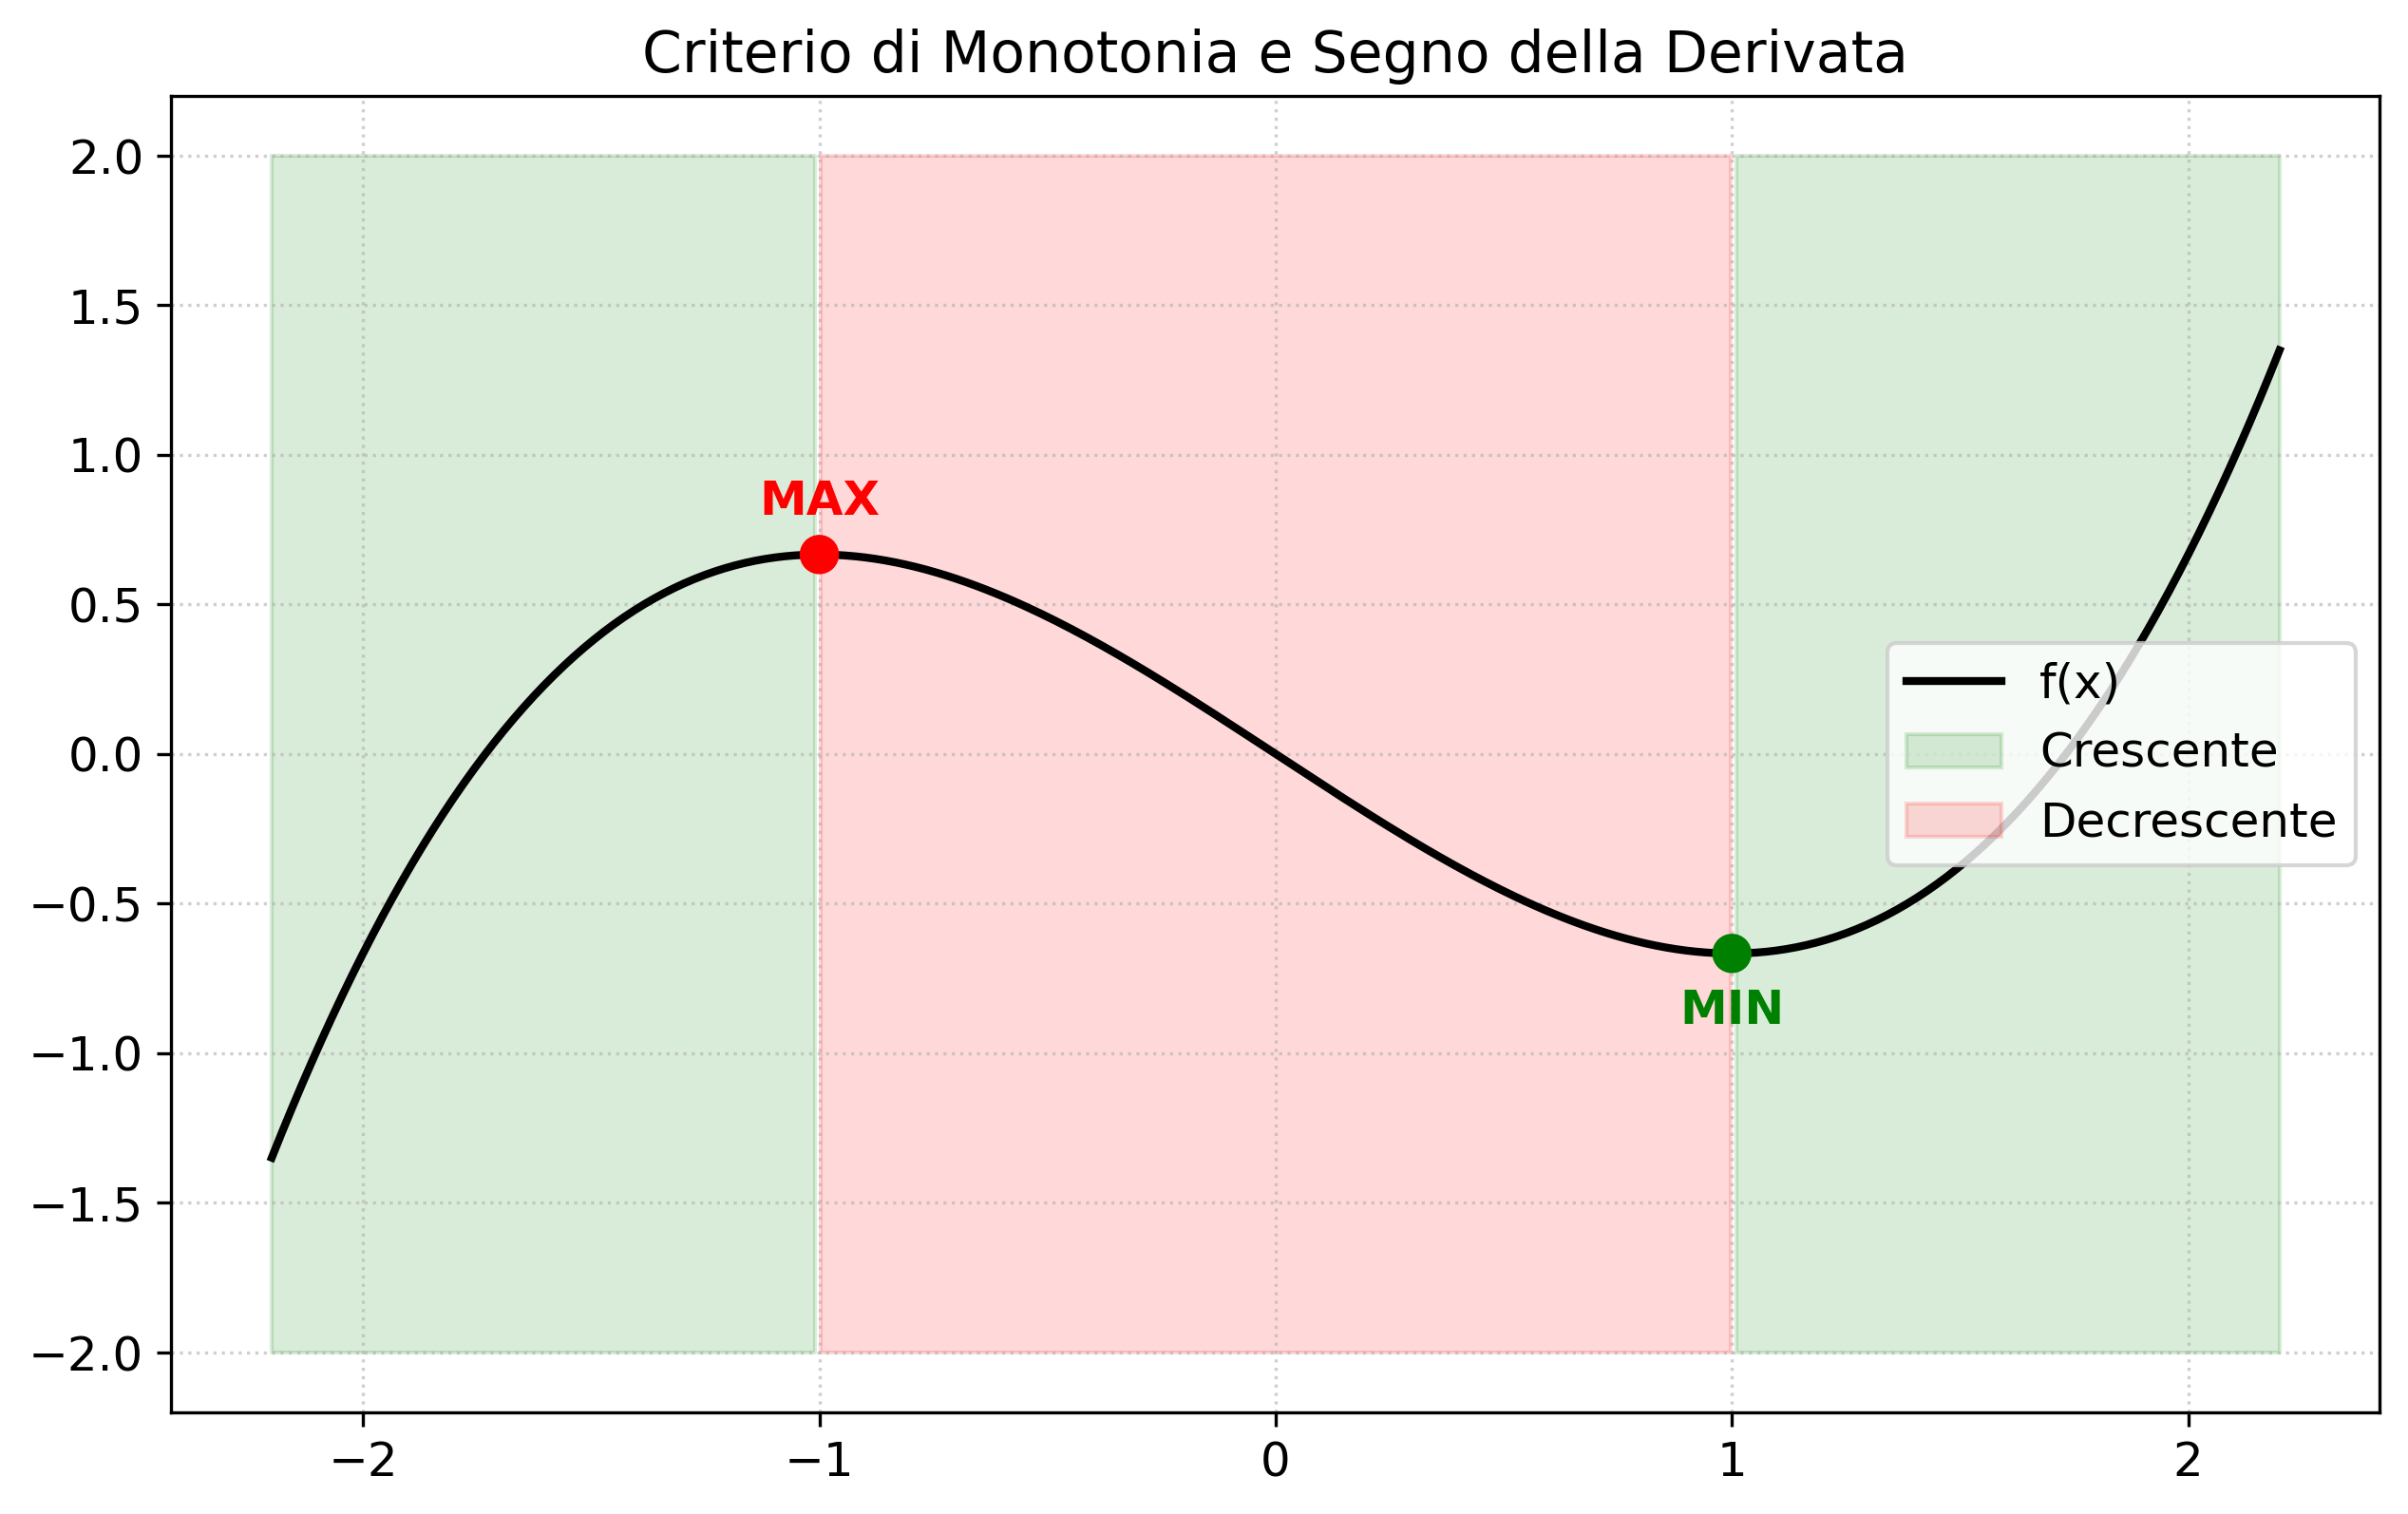
\includegraphics[width=0.7\textwidth]{img/monotonia_estremi.png}
    \end{center}
}

\pf{
    \begin{itemize}
        \item ($\implies$)
        \[ f'(x_{0})=\lim_{ h \to 0 } \frac{f(x_{0}+h)-f(x_{0})}{h}=\begin{dcases}
        h\to 0^+ \implies \frac{(+)}{(+)}\geq 0 \\
        h\to 0^- \implies \frac{(-)}{(-)}\geq 0 \\
        \end{dcases} \]
        \item ($\impliedby$) Hp $f'(x)\geq 0 \implies f \nearrow$.
        Siano $x_{1}<x_{2}$ e devo dimostrare che $f(x_{1})<f(x_{2})$.
        Applichiamo Lagrange in $[x_{1},x_{2}]\subseteq[a,b]$
        \[ \exists c \in ]x_{1},x_{2}[:\frac{f(x_{2})-f(x_{1})}{x_{2}-x_{1}}=f'(c)\geq 0 \]
    \end{itemize}
}

\subsection{Teorema di Caratterizzazione delle Funzioni Strettamente Monotone}

\thm{Caratterizzazione delle Funzioni Strettamente Monotone}{
    Sia $f:[a,b]\to \mathbb{R}$ continua.
    Sia $f$ derivabile in $]a,b[$.
    Allora: 
    \begin{enumerate}
        \item \[ f \nearrow_{S}\iff \begin{dcases}
        f'(x)\geq 0 \; \forall x \in ]a,b[ \\
        f' \text{ non si annulla in nessun sottointervallo in maniera costante}\\ \not \exists [c,d]\subseteq[a,b] : f' (x)=0 \; \forall x \in[c,d]
        \end{dcases} \] 
        \item \[ f \searrow_{S}\iff \begin{dcases}
        f'(x)\leq 0 \; \forall x \in ]a,b[ \\
        f' \text{ non si annulla in nessun sottointervallo in maniera costante}\\ \not \exists [c,d]\subseteq[a,b] : f' (x)=0 \; \forall x \in[c,d]
        \end{dcases} \]
    \end{enumerate}
}

\subsection{Condizione Sufficiente al Primo Ordine per gli Estremi Relativi}

\thm{Condizione Sufficiente al $1^{\circ}$ Ordine per gli Estremi Relativi}{
    Sia $f:[a,b]\to \mathbb{R}$ continua.
    Sia $f$ derivabile in $]a,b[$ escluso al più $x_{0}\in]a,b[$.
    Allora se:
    \begin{enumerate}
        \item \[ \begin{dcases}
        f'(x)\leq 0 \quad x <x_{0} \\
        f'(x)\geq 0 \quad x>x_{0}
        \end{dcases}\implies x_{0} \text{ è punto di \textit{Minimo relativo}} \]
        \item \[ \begin{dcases}
        f'(x)\geq 0 \quad x <x_{0} \\
        f'(x)\leq 0 \quad x>x_{0}
        \end{dcases}\implies x_{0} \text{ è punto di \textit{Massimo relativo}} \]
    \end{enumerate}
    \begin{center}
        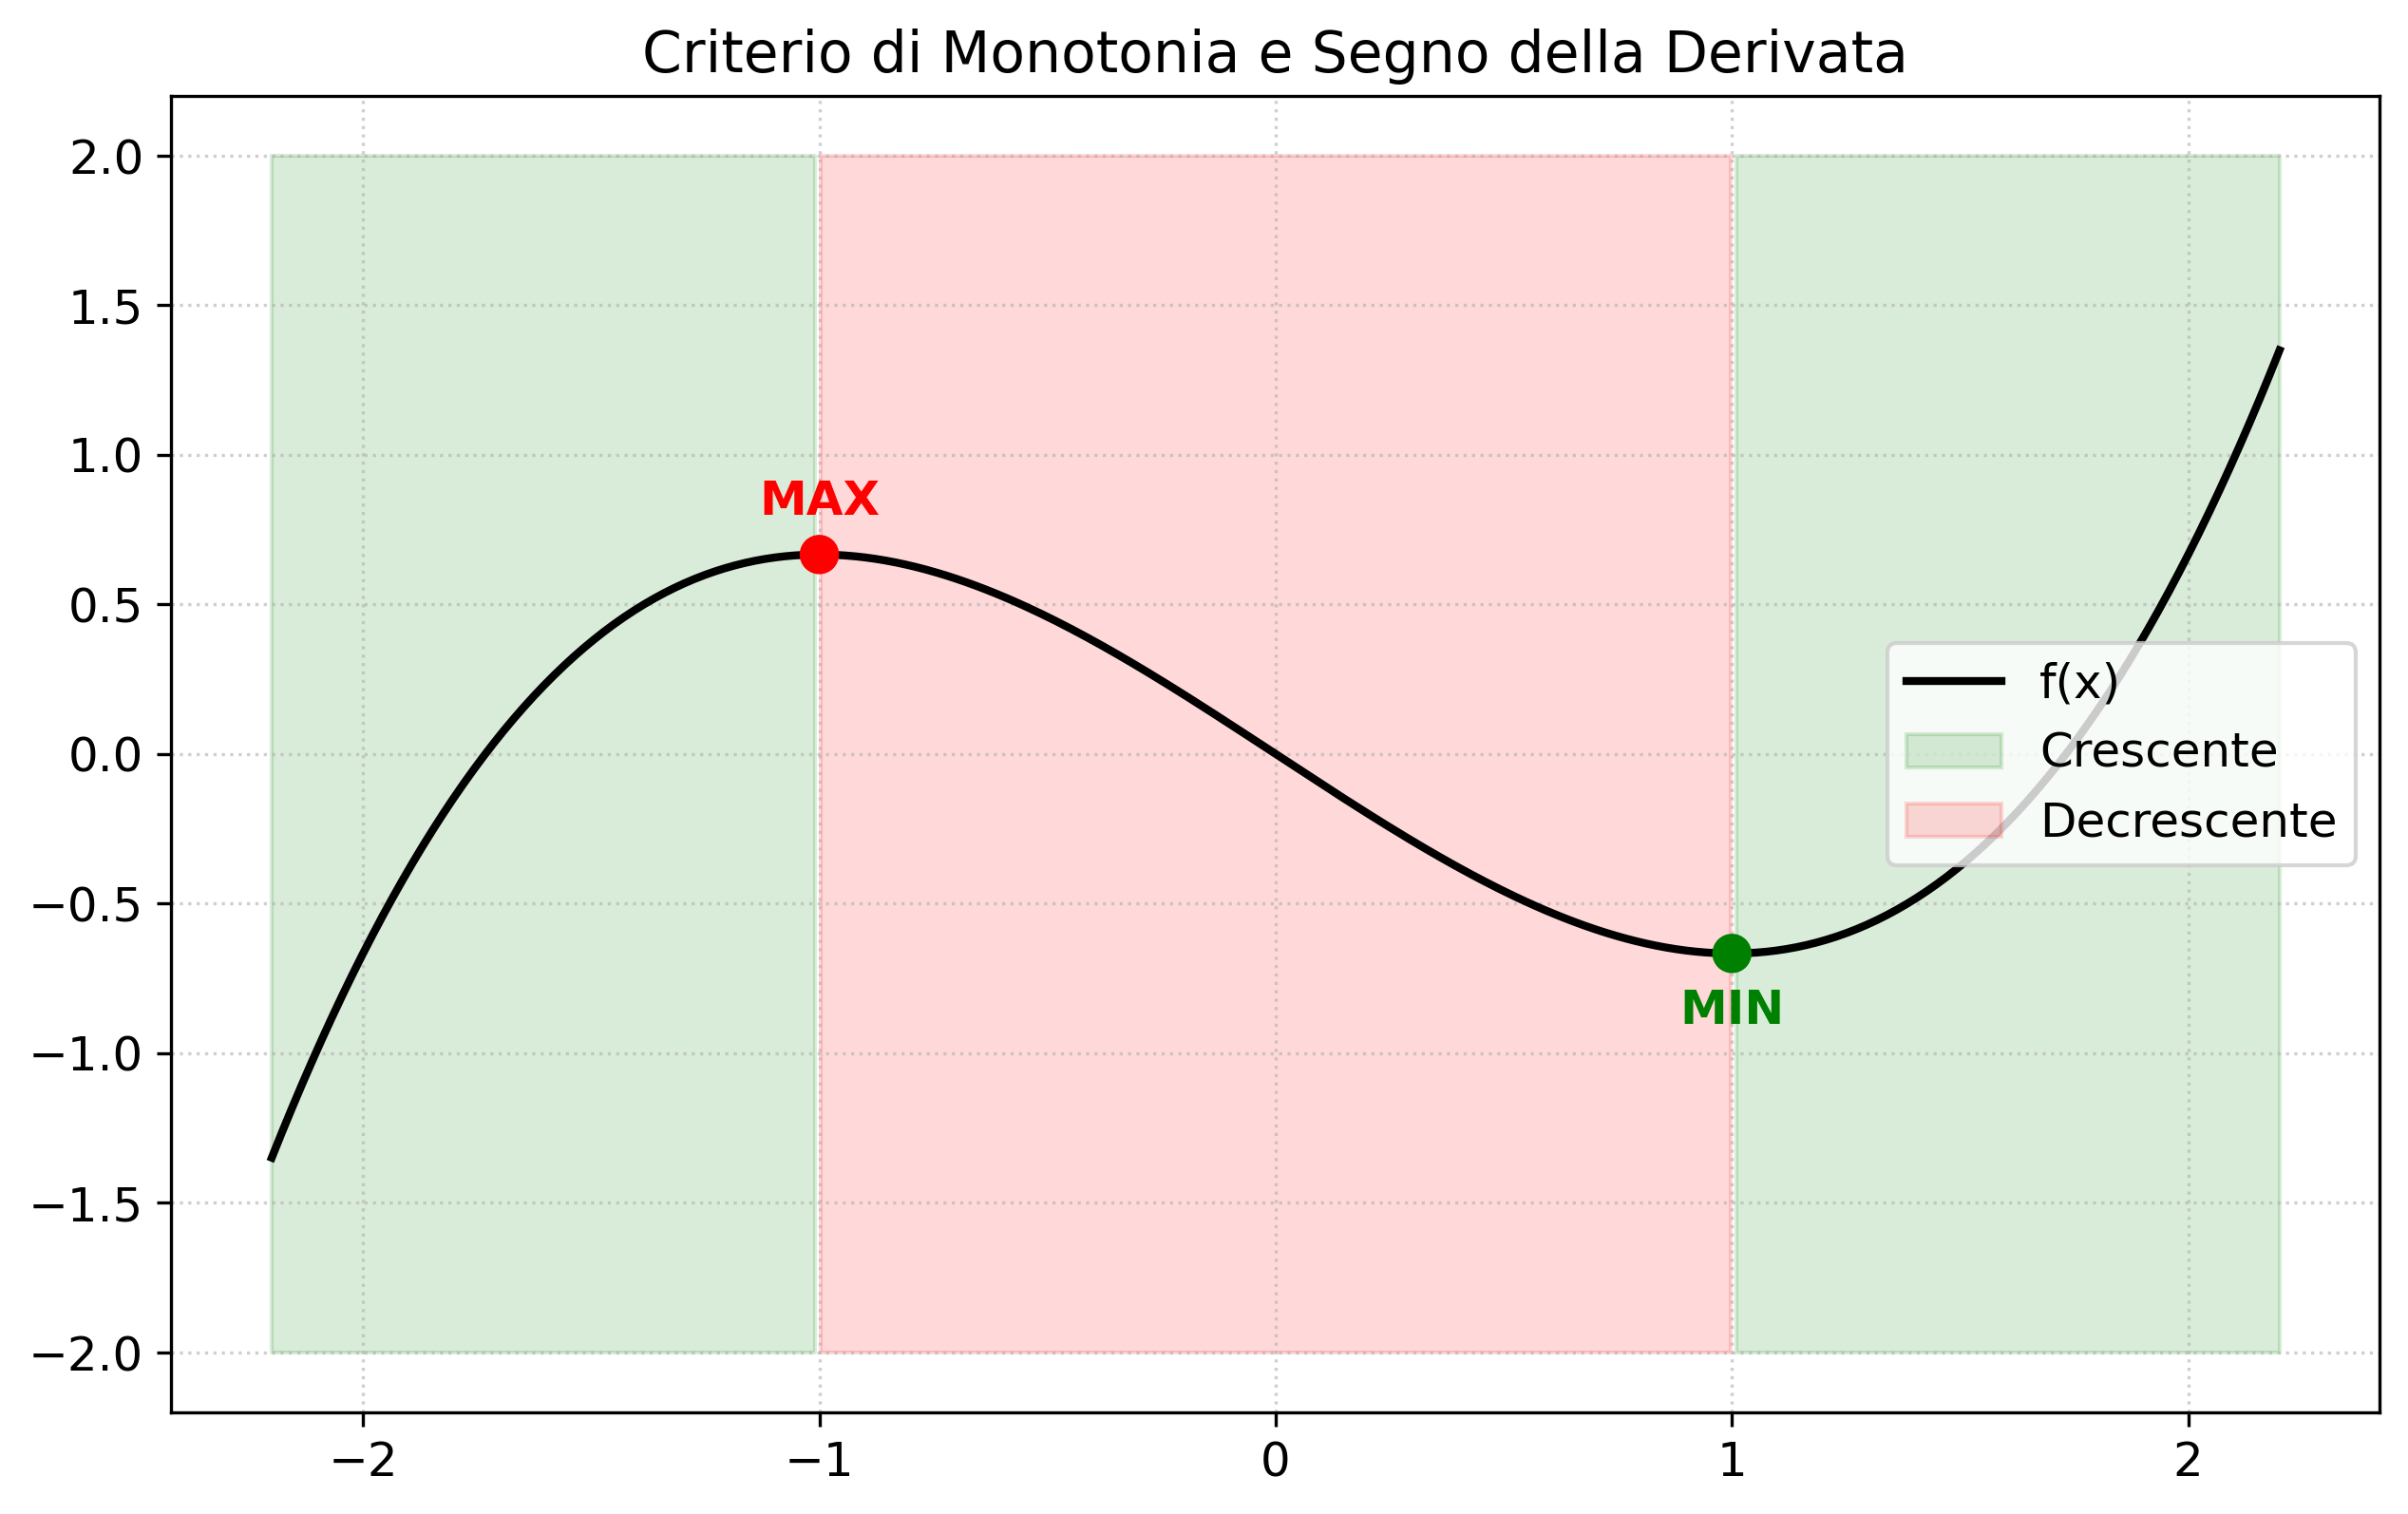
\includegraphics[width=0.7\textwidth]{img/monotonia_estremi.png}
    \end{center}
}

\subsection{Teoremi di de l'Hôpital}

\thm{1° Teorema di de l'Hôpital}{
    Siano $f,g$ derivabili in $]a,x_{0}[$ (con $x_{0}=+\infty$ eventualmente). Supponiamo che:
    \begin{enumerate}
        \item $\displaystyle \lim_{ x \to x_{0} } f(x)=\lim_{ x \to x_{0} } g(x)=0$
        \item $g'(x)\neq 0 \; \forall x \in ]a,x_{0}[$
        \item $\exists \lim_{ x \to x_{0} } \frac{f'(x)}{g'(x)}$
    \end{enumerate}
    Allora:
    \[ \lim_{ x \to x_{0} } \frac{f(x)}{g(x)}=\lim_{ x \to x_{0} } \frac{f'(x)}{g'(x)} \]
}

\ex{
    Esempio Utilizzo SBAGLIATO del Teo
    \begin{align*}
    & x_{0}=0\\
    &f(x)=x^2 \cos \frac{1}{x}\\
    & g(x)=e^x-1\to 0\\
    & \lim_{ x \to 0 } \frac{f'(x)}{g'(x)}=\lim_{ x \to 0 } \frac{2x \cos \frac{1}{x}+ \sin \frac{1}{x}}{e^x}= \not \exists \\
    & \lim_{ x \to 0 } \frac{f(x)}{g(x)}=0 
    \end{align*}
}

\pf{
    \begin{enumerate}
        \item Suppongo $x_{0} \in \mathbb{R}$ e usando la 1) prolungo $f,g$ in $x_{0}$.
        \item Osserviamo che $g(x)\neq 0\; \forall x \in ]a,x_{0}[$ perchè altrimenti Rolle andrebbe in contrasto con la 2) (delle hp).
        \item Sia $x_{n}\in]a, x_{0}[ \;\forall n$ e $x_{n}\to x_{0}$ e poniamo:
        \[ h(t)=f(t)g(x_{n})-g(t)f(x_{n}) \quad t \in]a,x_{0}[ \]
        Applico Rolle ad $h(t)$ in $[x_{n},x_{0}]$:
        \begin{itemize}
            \item $h(x_{n})=0$
            \item $h(x_{0})=0\implies \exists c_{n} \in ]x_{n}, x_{0}[:$
            \[ h'(c_{n})=0\implies 0=f'(c_{n})g(x_{n})-g'(c_{n})f(x_{n})\implies \frac{f'(c_{n})}{g'(c_{n})}=\frac{f(x_{n})}{g(x_{n})} \]
        \end{itemize}
    \end{enumerate}
}

\thm{2° Teorema di de l'Hôpital}{
    Se nella 1) del Teo di prima sostituiamo la seguente:
    \begin{itemize}
        \item[1b)] $\lim_{ x \to x_{0} } |f(x)|=\lim_{ x \to x_{0} } |g(x)|=+\infty$
        \item[2b)] ...
        \item[3b)] ...
    \end{itemize}
    $\implies$ Vale la stessa Tesi.
}
\chapter{Serie}

\section{Serie Numeriche}

\defn{Serie Numerica}{
    Sia $a_{n}$ una successione di numeri reali, si chiama \textbf{serie numerica di termine generale $a_{n}$} la seguente successione detta delle \textbf{somme parziali}.
    \begin{align*}
        & S_{1}=a_{1}\\
        & S_{2} = S_{1}+a_{2}=a_{1}+a_{2} \\
        & S_{3} = S_{2}+a_{3}=a_{1}+a_{2} +a_{3} \\
        & \vdots\\
        & S_{n} = S_{n-1}+a_{n} = a_{1}+a_{2}+a_{3}+\dots+a_{n}
    \end{align*}
    \[ S_{n}=\sum_{k=1}^{n} a_{k} \]
}

\subsection{Convergenza o divergenza}

\defn{Serie convergente}{
    Diremo che la serie \textbf{converge alla somma $S\in \mathbb{R}$} se $S_{n}$ è convergente a
    \[ \lim_{ n \to \infty }S_{n}=S \]
    e $S$ si indica con 
    \[ S=\sum_{n=1}^{+\infty} a_n \]
}

\defn{Serie divergente}{
    Diremo che la serie \textbf{diverge a $\pm \infty$} se
    \[ \lim_{ n \to \infty } S_{n}=\pm \infty \]
    rispettivamente:
    \[ \sum_{n=1}^{+\infty} a_{n}=\pm \infty \]
}

\defn{Serie Regolare}{
    Se la serie diverge o converge, diremo che è una serie regolare.
}

\defn{Serie Non Regolare}{
    Se: 
    \[ \lim_{ n \to \infty } S_{n} = \not \exists \]
    diremo che non è regolare.
}

D'ora in poi una serie di termine generale $a_{n}$ si indicherà con:
\[ \sum_{n=1}^{+\infty} a_{n} \]
studiare il \textbf{carattere} delle serie significa studiare se la serie:
\begin{itemize}
    \item converge
    \item diverge
    \item oscilla
\end{itemize}

\subsection{Esempi di tipi di Serie}

\subsubsection{Serie Geometrica}

\defn{Serie Geometrica}{
    Sia $q \in \mathbb{R}$.
    La serie geometrica di ragione $q$:
    \[ \sum_{n=0}^{+\infty} q^n = 1 + q+ q^2 + \dots \]
    Si chiama così perché ricorda la progressione geometrica.
}

\ex{
    Progressione geometrica:
    \[
    S_{n}=\begin{dcases}
    \frac{1-q^{n+1}}{1-q} \qquad q\neq 1 \\
    \text{Sommo sempre 1 } \quad q=1
    \end{dcases}
    \]
    \[
    \lim_{ n \to \infty } S_{n}= \begin{dcases}
    \frac{1}{1-q} =S \quad &|q|<1 \\
    \not \exists & q \le -1 \\
    +\infty & q\ge 1
    \end{dcases}
    \]
}

\ex{
    \[
    \begin{drcases}
    & 0,\overline{9}=0,9+0,09+0,009+0,0009+\dots = \\
    & =\frac{9}{10} + \frac{9}{100}+\frac{9}{1000} + \dots + \frac{9}{10^n}= \\
    & = \frac{9}{10}\left( 1 +\frac{1}{10} +\frac{1}{100} + \dots \right) = \frac{9}{10}\left( \frac{1}{1-\frac{1}{10}} \right)=\frac{9}{10} \left(\frac{10}{9}\right) = 1
    \end{drcases}0,\overline{9}=1
    \]
}

\subsubsection{Serie Armonica}
\[ \sum_{n=1}^{+\infty} \frac{1}{n} = +\infty \]

\pf{
    \begin{align*}
    & \left( 1+\frac{1}{n} \right)^n<e\\
    & \log\left( 1+\frac{1}{n} \right)^n < \log e \implies \log\left( 1+\frac{1}{n} \right) < \frac{1}{n} \\
    & \underbrace{\log(n+1) - \log n }_{a_{n}}< \frac{1}{n} \\
    & \sum_{k=1}^{n} \log(k+1)-\log k < \sum_{k=1}^{n} \frac{1}{k}\\
    & b_{n} <c_{n}\\
    & \text{Se dimostro che } b_{n} \to +\infty \text{ per il teorema del confronto:} \\
    & \underbrace{\cancel{ \log 2 } - \log 1}_{b_{1}} + \underbrace{{\cancel{ \log 3 } - \cancel{ \log 2 }}}_{b_{2}} + \underbrace{{\cancel{ \log 4 } - \cancel{ \log 3}}}_{b_{3}} + \dots + \log(n+1) - \cancel{ \log n } = b_{n}\\ 
    & b_{n} = \sum_{k=1}^{n} \log(k+1) - \log k = \log(n+1)\\
    & \text{La serie armonica diverge a } +\infty
    \end{align*}
}

\subsubsection{Serie di Mengoli}
\[ \sum_{n=1}^{+\infty} \frac{1}{n(n+1)}=1 \]
\[ \sum_{n=1}^{+\infty} \frac{1}{n}-\frac{1}{n+1} \]
\begin{align*}
    & S_{n}=\sum_{k=1}^{n} \frac{1}{k}-\frac{1}{k+1}=\\
    & = \left( 1 -\cancel{ \frac{1}{2} }\right) + \left( \cancel{ \frac{1}{2} } -\cancel{ \frac{1}{3} } \right) + \left( \cancel{ \frac{1}{3} } -\cancel{ \frac{1}{4} } \right) + \dots \left( \cancel{ \frac{1}{n} } -\frac{1}{n+1} \right)= 1- \frac{1}{n+1}\\
    & \lim_{n \to +\infty} S_n = \lim_{n \to +\infty} \left( 1 - \frac{1}{n+1} \right) = 1
\end{align*}

\subsubsection{Serie Telescopiche}
\[ \sum_{n=1}^{+\infty} (a_{n}-a_{n+1})=a_{1}-\textcolor{orange}{\boxed{\lim_{ n \to +\infty } a_{n+1}}} \]
\[ \textcolor{orange}{\text{La serie e la sua ragione hanno lo stesso carattere: NON limite, ma carattere}} \]
\[ S_{n}=a_{1}-a_{n} \]

\thm{Condizione necessaria per la convergenza}{
    Sia $\displaystyle \sum_{n=1}^{+\infty} a_{n}$ con $a_{n}$ una successione.
    \[ \text{Se } \sum_{n=1}^{+\infty} a_{n} \text{ converge } \implies a_{n}\to 0 \quad (\centernot\impliedby \text{ vedi serie armonica}) \]
}

\pf{
    $a_{n}=S_{n}-S_{n-1}\to S-S = 0$. Non è forma indeterminata perché converge.
}

\thm{Criterio di Convergenza di Cauchy}{
    La serie:
    \[ \sum_{n=1}^{+\infty} a_{n} \text{ conv. } \iff \forall \epsilon> 0 \exists \nu > 0 : |a_{n+1}+a_{n+2}+\dots+a_{n+p}|<\epsilon \quad \forall n > \nu \; \forall p \in \mathbb{N} \]
}

\pf{
    (Per casa)
    $|S_m- S_n| < \epsilon \; \forall n, m > \nu$
    
    \textbf{CONTINUA PER ESERCIZIO}
}

\section{Serie a Termini Non Negativi}

\prop{
    Consideriamo $\displaystyle \left( \sum_{n=1}^{+\infty} a_{n} \; , \; a_{n}\geq 0 \right)$.
    \[ \text{Se }a_{n}\geq 0 \implies \sum_{n=1}^{+\infty} a_{n} \text{ è regolare} \]
}

\pf{
    \[ S_{n}=S_{n-1}+\underbrace{a_{n}}_{\geq 0}\geq S_{n-1} \]
    Allora $S_{n}$ è regolare ($\nearrow$).
}

\ex{
    \begin{itemize}
        \item $\displaystyle \sum_{n=1}^{+\infty} \frac{\sqrt[n]{n!}}{\sqrt{ n }}= +\infty \quad \text{perchè } a_{n} \text{ non tende a 0}$
        \item $\displaystyle \sum_{n=1}^{+\infty} \frac{1}{n}= +\infty \quad \text{anche se } a_{n} \to 0 \text{ (è una condizione necessaria ma non sufficiente)}$
    \end{itemize}
}

\thm{Criterio del confronto (per le serie)}{
    Siano $a_{n},b_{n}\geq 0 \; \forall n$ e sia verificata:
    \[ a_{n}\leq b_{n} \text{ definitivamente} \]
    Allora valgono le seguenti:
    \begin{enumerate}
        \item $\displaystyle \text{Se } \sum_{n=1}^{+\infty} b_{n} \text{ conv.} \implies \sum_{n=1}^{+\infty} a_{n} \text{ conv.}$
        \item $\displaystyle \text{Se } \sum_{n=1}^{+\infty} a_{n} \text{ diverge a } +\infty \implies \sum_{n=1}^{+\infty} b_{n} \text{ diverge a } +\infty$
    \end{enumerate}
}

\pf{
    $S_{n}\leq T_{n} \implies \sum a_{n} \leq \sum b_{n}$
}

\ex{
    \[ \sum_{n=1}^{+\infty} \frac{1}{n^3} \implies \sum_{n=1}^{+\infty} \frac{1}{n^3}<\sum_{n=1}^{+\infty} \frac{1}{n(n+1)} \]
    Dato che $\sum \frac{1}{n(n+1)}$ converge, convergono entrambe.
}

\rmkb{
    \[ \boxed{0<\alpha<1} \]
    \[ \sum_{n=1}^{+\infty} \frac{1}{n^\alpha} > \sum_{n=1}^{+\infty} \frac{1}{n} \]
    Divergono entrambe.
}

\section{Criteri del Confronto Asintotico}

\thm{Criterio del Confronto Asintotico I}{
    Siano $a_{n},b_{n}\geq 0 \; \forall n$.
    \[ \text{Se } \lim_{ n \to \infty } \frac{a_{n}}{b_{n}}=l \in ]0. +\infty[ \]
    Allora le serie $\sum_{n=1}^{+\infty}a_{n}$ e $\sum_{n=1}^{+\infty} b_{n}$ hanno lo stesso carattere.
    Posso scrivere:
    \[ \sum a_{n} \sim \sum b_{n} \]
}

\ex{
    \begin{itemize}
        \item $\displaystyle \sum_{n=1}^{+\infty} \sin \frac{1}{n} = +\infty$
        perchè se $\displaystyle \sum_{n=1}^{+\infty} \frac{1}{n}\implies \lim_{ n \to +\infty } \frac{\sin \frac{1}{n}}{\frac{1}{n}}=1$
        \item $\displaystyle \sum \log\left( 1+ \frac{1}{n} \right) = \sum \sin \frac{1}{n} = +\infty$
        \item $\displaystyle \sum \frac{1}{\sqrt[n]{n!}} = (\text{Come l'armonica?})$
        \item $\displaystyle \sum_{n=1}^{+\infty} \left( 1-\cos \frac{1}{n} \right) \sim \sum_{n=1}^{+\infty} \frac{1}{2n^2} \implies \text{Convergono}$
        \item 
        \begin{align*}
        &\sum_{n=1}^{+\infty} \left( \underbrace{\left( e^{\frac{1}{n}-1} \right)}_{\alpha=1 \; l=1}-\underbrace{\frac{1}{n}}_{{\alpha=1 \; l=1}} \right) \implies \text{Uso Taylor} \implies\sim \sum \frac{1}{n^2} \implies \text{Converge} \implies \\
        & \implies \lim_{ n \to +\infty } \frac{e^{\frac{1}{n}}-1- \frac{1}{n}}{\frac{1}{n^2}} = \lim_{ n \to +\infty } \frac{1+ \frac{1}{n}+ \frac{1}{2n^2} + o\left( \frac{1}{n^2} \right)- 1 - \frac{1}{n}}{\frac{1}{n^2}} =\\
        & =\lim_{ n \to +\infty } \frac{\frac{1}{2n^2}}{\frac{1}{n^2}}=\frac{1}{2} 
        \end{align*}
    \end{itemize}
}

\pf{
    Per Hp:
    \[ \lim_{ n \to +\infty } \frac{a_{n}}{b_{n}} = l > 0 \text{ e } l<+\infty \]
    \[ \forall \epsilon>0 \exists \nu \in \mathbb{N}: l- \epsilon < \frac{a_{n}}{b_{n}} < l + \epsilon \]
    \[ (l-\epsilon)b_{n}<a_{n}<(l+\epsilon)b_{n} \; \forall n > \nu \]
}

\rmkb{
    \[
    \sum_{n=1}^{+\infty} \frac{1}{n^\alpha}=\begin{dcases}
    \alpha\geq 2 \implies \text{Converge} \\
    \text{?} \\
    \alpha=1 \implies \text{Diverge a }+\infty
    \end{dcases}
    \]
}

\prop{
    \textbf{Serie Armonica Generalizzata} \\
    Si consideri la serie:
    \[ \sum_{n=1}^{+\infty} \frac{1}{n^\alpha} \; , \; \alpha \in \mathbb{R} \]
    Allora essa converge $\forall \alpha>1$
    e diverge positivamente $\forall \alpha \leq 1$.
}

\pf{
    (Presente sul Pagani-Salsa) 
    $a_{n}=\frac{1}{n^\alpha}$
    $\alpha>1$
    \begin{align*}
    & S_{2^n -1}=a_{1}+a_{2}+\dots+a_{2^n -1}=\\
    &=1 + \underset{ <2 \cdot \frac{1}{2^\alpha} }{ \textcolor{red}{\boxed{\frac{1}{2^\alpha} +\frac{1}{3^\alpha}}} } +\underset{ < 4 \cdot \frac{1}{4^\alpha} }{ \textcolor{orange}{\boxed{\frac{1}{4^\alpha} +\frac{1}{5^\alpha} +\frac{1}{6^\alpha} +\frac{1}{7^\alpha}}} }+\dots+\\
    & + \frac{1}{(2^{n-1})^\alpha} +\frac{1}{(2^{n-1}+1)^\alpha}+\dots+\frac{1}{(2^{n}-1)^\alpha}
    \end{align*}
    La maggioro $\implies$
    \[ < 1 + \textcolor{red}{\frac{1}{2^{(\alpha-1)}}}+\textcolor{orange}{\frac{1}{2^{2(\alpha-1)}}} +\frac{1}{2^{3(\alpha-1)}}+\dots +\frac{1}{2^{(n-1)(\alpha-1)}}= \sum_{n=0}^{+\infty} \left( \frac{1}{2^{(\alpha-1)}} \right)^n \implies \text{Converge} \]
}

\thm{Criterio Del Confronto Asintotico II}{
    Siano $a_{n}\geq 0, b_{n}>0$. Allora si hanno le seguenti:
    \begin{enumerate}
        \item $\displaystyle \lim_{ n \to +\infty } \frac{a_{n}}{b_{n}}=0$
        (Utile se $a_{n}\to 0$ e $b_{n}\to 0$)
        \begin{itemize}
            \item Se $\sum b_{n}$ converge $\implies \sum a_{n}$ converge
            \item Se $\sum a_{n}$ diverge $\implies \sum b_{n}$ diverge
            \item Esempio b: $\sum \frac{1}{n} =+\infty \implies \sum \frac{1}{\sqrt{ n }}=+\infty$
        \end{itemize}
        \item $\displaystyle \text{Se } \lim_{ n \to +\infty } \frac{a_{n}}{b_{n}} = +\infty$
        Allora: 
        \begin{itemize}
            \item Se $\sum b_{n}$ Div. $\implies \sum a_{n}$ Div.
            \item Se $\sum a_{n}$ Conv. $\implies \sum b_{n}$ Conv.
        \end{itemize}
    \end{enumerate}
}

\pf{
    (Dimostrazione 1)
    \[ \forall \epsilon>0 \exists \nu>0 : 0 \leq \frac{a_{n}}{b_{n}}<\epsilon \quad \forall n > \nu \]
    Scelto $\epsilon=1$ allora $\exists \nu>0:$
    \[ 0\leq a_{n}< b_{n} \quad \forall n>\nu \]
}

\ex{
    \[ \sum_{n=2}^{+\infty} \frac{1}{n^2 \log n} \]
    \[ \sum b_{n}= \sum \frac{1}{n^2} \]
    \[ \lim_{ n \to +\infty } \frac{\cancel{ n^2 }}{\cancel{ n^2 } \log n}=0 \]
}

\subsection{Teorema Criterio degli Infinitesimi}

\thm{Teorema Criterio degli Infinitesimi}{
    Sia $a_{n}\geq 0$ e tale che: 
    \[ \lim_{ n \to +\infty } n^\alpha a_{n} = l\in[0,+\infty] \]
    Allora:
    \begin{enumerate}
        \item Se $0<l<+\infty \implies$
        \begin{itemize}
            \item $\alpha>1\implies \sum a_{n}$ converge.
            \item $\alpha\leq1\implies \sum a_{n}$ diverge.
        \end{itemize}
        \item Se $l=0$ e $\alpha>1 \implies \sum a_{n}$ converge.
        \item Se $l=+\infty$ e $\alpha \leq 1 \implies \sum a_{n}$ diverge.
    \end{enumerate}
}

\ex{
    \begin{itemize}
        \item $\displaystyle \sum_{n=1}^{+\infty} \frac{1}{\sqrt{ n }+2}=+\infty \sim \sum_{n=1}^{+\infty} \frac{1}{\sqrt{ n }} = +\infty \; \text{Perchè } \alpha=\frac{1}{2}$
        \item $\displaystyle \sum_{n=1}^{+\infty} \underbrace{ \sqrt{ n^3 +3n }- \sqrt{ n^3 +2 } }_{a_{n}}$
        \[ \lim_{ n \to +\infty } \frac{n^3 +3n - ( n^3 +2 )}{\sqrt{ n^3 +3n }+ \sqrt{ n^3 +2 }}=\frac{3n-2}{\sqrt{ n^3 +3n } + \sqrt{ n^3 +2 }}= \frac{n(\dots)}{n^{\frac{3}{2}}(\dots)}= \frac{1}{\sqrt{ n }}=0 \]
        \[ \text{Allora } \sum_{n=1}^{+\infty} a_{n} \sim \sum_{n=1}^{+\infty} \frac{1}{\sqrt{ n }}=+\infty \]
    \end{itemize}
}

\subsection{Esempi che non rispettano le Hp precedenti}
\begin{itemize}
    \item $\displaystyle \sum_{n=1}^{+\infty} \frac{n!}{n^n}$
    \item $\displaystyle \sum_{n=1}^{+\infty} \frac{n^n}{3^{n^2}}$
    \item $\displaystyle \sum_{n=1}^{+\infty} \frac{2^n}{n!}$
    \item $\displaystyle \sum_{n=1}^{+\infty} \frac{(2n)!}{(2n)^n}$
\end{itemize}

\subsection{Criterio della Radice per le Serie}

\thm{Criterio della Radice per le Serie}{
    Sia $a_{n}\geq 0$.
    Allora se
    \[ \lim_{ n \to +\infty } \sqrt[n]{a_{n}}=l \]
    Si ha:
    \begin{enumerate}
        \item se $l>1 \implies \sum a_{n}$ diverge a $+\infty$
        \item se $l<1 \implies \sum a_{n}$ converge
    \end{enumerate}
}

\pf{
    \begin{enumerate}
        

    \item Se $l>1$ prendo $\epsilon>0: \quad l-\epsilon>1$.
    Per la definizione di limite:
    \[ \exists \nu>0 : (l- \epsilon) < \sqrt[n]{a_{n}} < (l+\epsilon) \]
    Elevo ad n:
    \[ \exists \nu>0 : (l- \epsilon)^{\textcolor{orange}{n}} < a_{n} < (l+\epsilon)^{\textcolor{orange}{n}} \]
    
    
    \item Sia $0\overset{\text{T.p.s}}{ \leq } l < 1$.
    Sia $\epsilon: l +\epsilon < 1$.
    Poiché:
    \[ \lim_{ n \to +\infty } \sqrt[n]{a_{n}}=l \]
    allora risulta $\exists \nu>0:$
    \[ 0\leq \sqrt[n]{a_{n}}< l +\epsilon\implies 0\leq a_{n} < (l+\epsilon)^n \; \forall n > \nu \]
    Poiché $l+\epsilon<1\implies \sum(l+\epsilon)^n$ converge.
    La dimostrazione segue dal teorema del confronto per le serie.
 
    \end{enumerate}
}

\ex{
    \[ \sum_{n=1}^{+\infty} \frac{n!}{n^n} \quad a_{n}\geq 0 \]
    Criterio della Radice:
    \[ \lim_{ n \to +\infty } \sqrt[n]{\frac{n!}{n^n}}=\lim_{ n \to +\infty } \frac{\sqrt[n]{n!}}{n}=\frac{1}{e} < 1 \]
}

\thm{Criterio del Rapporto per le Serie}{
    Sia $a_{n}> 0$ e tale che esista:
    \[ \lim_{ n \to +\infty } \frac{a_{n+1}}{a_{n}}=l \]
    Allora:
    \begin{enumerate}
        \item $\text{Se } l>1\implies \sum_{n=1}^{+\infty} a_{n}=+\infty$
        \item $\text{Se }l<1 \implies \sum_{n=1}^{+\infty} a_{n} \text{ converge}$
    \end{enumerate}
}

\pf{
    Segue dal Criterio Rapporto radice per le Successioni.
}

\subsubsection{Costante di Eulero Mascheroni}

\thm{Costante di Eulero Mascheroni}{
    La successione:
    \[ \left( \sum_{k=1}^{n} \frac{1}{k} \right)-\log n \]
    converge ad un numero finito non nullo che chiameremo:
    \[ \gamma = \text{ costante di Eulero Mascheroni} \approx 0,577 \]
    \[ \lim_{ n \to +\infty } \frac{S_{n}}{\log n}=\lim_{ n \to +\infty } \frac{S_{n}-\log n +\log n}{\log n}=\lim_{ n \to +\infty } \frac{S_{n}-\log n}{\log n}+1=1 \]
}

\section{Serie a Segni Alterni}

\defn{Serie a Segni Alterni}{
    Sia $a_{n}\geq 0\; \forall n$, la serie:
    \[ \sum_{n=1}^{+\infty} (-1)^{n-1} a_{n}=a_{1}-a_{2}+a_{3}-a_{4}+\dots \]
    Si chiama \textbf{serie a segni alterni} di termine generale $a_{n}$.
}

\ex{
    \begin{itemize}
        \item $\displaystyle \sum_{n=1}^{+\infty} \frac{(-1)^{n-1}}{n}=1 -\frac{1}{2}+\frac{1}{3}-\frac{1}{4}+\dots \qquad \text{Serie armonica a segni alterni}$
        \item $\displaystyle \sum_{n=1}^{+\infty} (-1)^n \arcsin\left( \frac{1}{n} \right)= -\arcsin 1 +\arcsin \frac{1}{2} - \dots$
    \end{itemize}
}

\subsection{Criterio di Leibniz}

\thm{Criterio di Leibniz}{
    \begin{enumerate}
        \item Sia $a_{n}\geq 0$
        \item Sia $a_{n} \searrow$ (decrescente)
        \item Sia $a_{n}$ infinitesima $\left(\displaystyle \lim_{ n \to +\infty }a_{n}=0\right)$
    \end{enumerate}
    \[ \text{Allora } \sum_{n=1}^{+\infty} (-1)^{n-1}a_{n} \text{ converge} \]
    Inoltre, detta $S$ la sua somma, si ha la seguente:
    \[ |S-S_{n}|\leq a_{n+1} \quad (\text{Stima del resto}) \]
}

\pf{
    Considero $S_{2n}$ e $S_{2n+1}$.
    Dimostro che sono convergenti allo stesso limite.
    1) Dimostriamo che $S_{2n}$ e $S_{2n+1}$ sono monotone e limitate.
    \[ S_{\underbracket{2n+2}}=S_{2n} \underbrace{+ a_{2n+1}-a_{2n+2} }_{{\geq 0 \; (a_{n} \searrow)}}\geq S_{\underbracket{2n}} \quad \nearrow \]
    \[ S_{\underbracket{2n+1}}=S_{2n-1}\underbrace{ - a_{2n}+a_{2n+1} }_{{\leq 0}}\leq S_{\underbracket{2n-1}} \quad \searrow \]
    $S_{2n} \nearrow \quad S_{2n+1}\searrow$
    Allora:
    \[ S_{3}\geq S_{2n+1}\geq S_{2n}\geq S_{2}\implies\text{ quindi } S_{2n} \text{ e } S_{2n+1} \text{ sono anche limitate.} \]
    $\implies$ sono convergenti per il Teorema delle Successioni monotone.
    Ma poiché:
    \[ S_{2n+1}-S_{2n}=a_{2n+1} \]
    Al limite per $n\to + \infty$:
    \[ S_{d}-S_{p}= 0 \implies S_{d}=S_{p}=\boxed{S} \]
    \[ \inf \{S_{2n+1}\} = S = \sup \{S_{2n}\} \]
    \[
    |S-S_{n}|=\begin{dcases}
    n \text{ pari} \\
    n \text{ dispari}
    \end{dcases}
    \]
    \begin{align*}
    &|S-S_{2n}| \underset{\substack{\text{(perché } S \\ \text{è il sup)}}}{=} S- S_{2n} \\
    & S - S_{2n} \underset{S \text{ è inf}}{\leq} S_{2n+1}-S_{2n}=a_{2n+1}\\
    & |S-S_{2n+1}| \underset{S \text{ è inf}}{=} S_{2n+1}-S \leq S_{2n+1}-S_{2n+2}=+a_{2n+2}
    \end{align*}
}

\ex{
    \[ \sum_{n=1}^{+\infty} \frac{(-1)^{n-1}}{n} \; \text{ Converge} \]
}

\subsection{Assoluta Convergenza}

\defn{Successione Assolutamente Convergente}{
    Sia $a_{n}$ una successione.
    La serie $\displaystyle \sum_{n=1}^{+\infty} a_{n}$ si dice \textbf{assolutamente convergente} se converge:
    \[ \sum_{n=1}^{+\infty} |a_{n}| \]
}

\rmkb{
    La convergenza finora citata è detta \textbf{convergenza semplice}.
}

\prop{
    Se $\displaystyle \sum_{n=1}^{+\infty} a_{n}$ converge assolutamente (ovvero se $\sum |a_{n}|$ converge)
    \[ \implies \sum_{n=1}^{+\infty} a_{n} \text{ converge} \]
    ($\centernot\impliedby$ Esempio: Armonica a segni alterni)
}

\ex{
    \[ \sum_{n=1}^{+\infty} \left|\frac{(-1)^n - n +1}{n^3+2n}\right|\leq \sum \frac{n+2}{n^3 +2n} \sim \sum \frac{1}{n^2} \]
}

\pf{
    \[ \Big||a_{n+1}|+|a_{n+2}|+\dots+|a_{n+p}|\Big|<\epsilon \quad \forall n>\nu \quad \forall p \in \mathbb{N} \]
    \[ \Big||a_{n+1}+a_{n+2}+\dots+a_{n+p}|\Big|<\Big||a_{n+1}|+|a_{n+2}|+\dots+|a_{n+p}|\Big| \]
    \[ \implies\left|a_{n+1}+a_{n+2}+\dots+a_{n+p}\right|<\Big||a_{n+1}|+|a_{n+2}|+\dots+|a_{n+p}|\Big| \]
}

\chapter{Integrali}
\section{I Problemi del Calcolo Integrale}
L'integrale nasce per risolvere due problemi:
\begin{enumerate}
    \item Area dei rettangoloidi.
    \begin{center}
    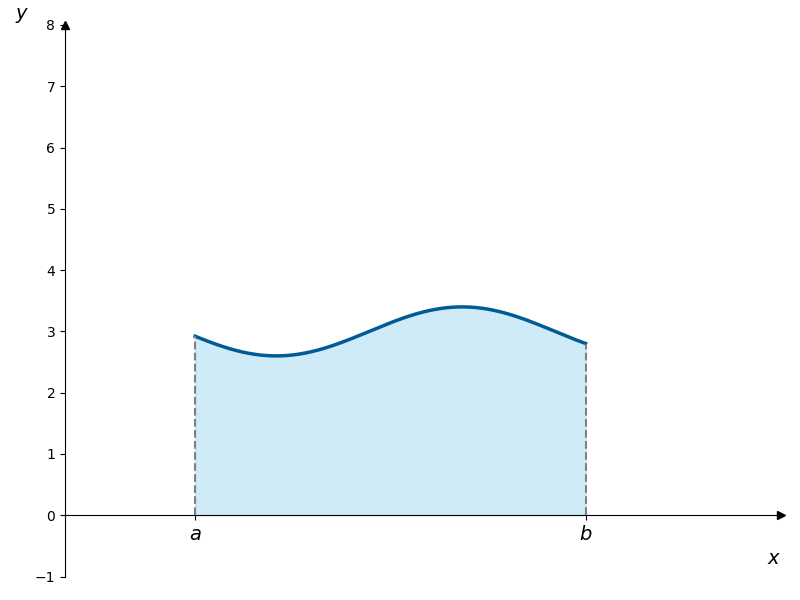
\includegraphics[width=0.7\textwidth]{img/rettangoloide.png}
    \end{center}
    \item Assegnata $f$:
    \[
    \exists F : F' = f
    \]
\end{enumerate}

\section{Integrale Definito}
Archimede ha calcolato l'area del settore parabolico "imprigionandola" tra due approssimazioni:
\begin{itemize}
    \item \textbf{Sottostima}: Ha sommato le aree di rettangoli inscritti (dentro la curva), ottenendo un valore inferiore a quello reale.
    \item \textbf{Sovrastima}: Ha sommato le aree di rettangoli circoscritti (fuori dalla curva), ottenendo un valore superiore.
\end{itemize}

\defn{Somma integrale superiore ed inferiore}{
    Sia $f: [a,b]\to \mathbb{R}$ limitata. Si definisce partizione di $[a,b]$ l'insieme:
    \[ P = \{ x_{0}=a, x_1 , x_2 , \dots , x_n = b : x_0 =a < x_1 < x_2 < \dots < x_n = b \} \]
    Consideriamo un generico intervallo $[x_k , x_{k+1}]$.
    Chiamiamo $m_k = \inf_{[x_k , x_{k+1}]} f(x)$ e $M_k = \sup_{[x_k , x_{k+1}]} f(x)$ che sono finiti essendo $f$ limitata.
    
    Si definisce \textbf{somma integrale inferiore} di $f$, relativa a $P$, la seguente:
    \[ s(P,f) = \sum_{k=0}^{n-1} m_k \cdot (x_{k+1} - x_k )= \sum_{k=1}^{n} m_k (x_k - x_{k-1}) \]
    Si definisce \textbf{somma integrale superiore} di $f$, relativa a $P$, la seguente:
    \[ S(P,f) = \sum_{k=0}^{n-1} M_k \cdot (x_{k+1} - x_k )= \sum_{k=1}^{n} M_k (x_k - x_{k-1}) \]
    Ovviamente $s(P,f)\leq S(P,f)$. Devo dimostrare $s \nearrow$ e $S \searrow$.
}

    \begin{center}
    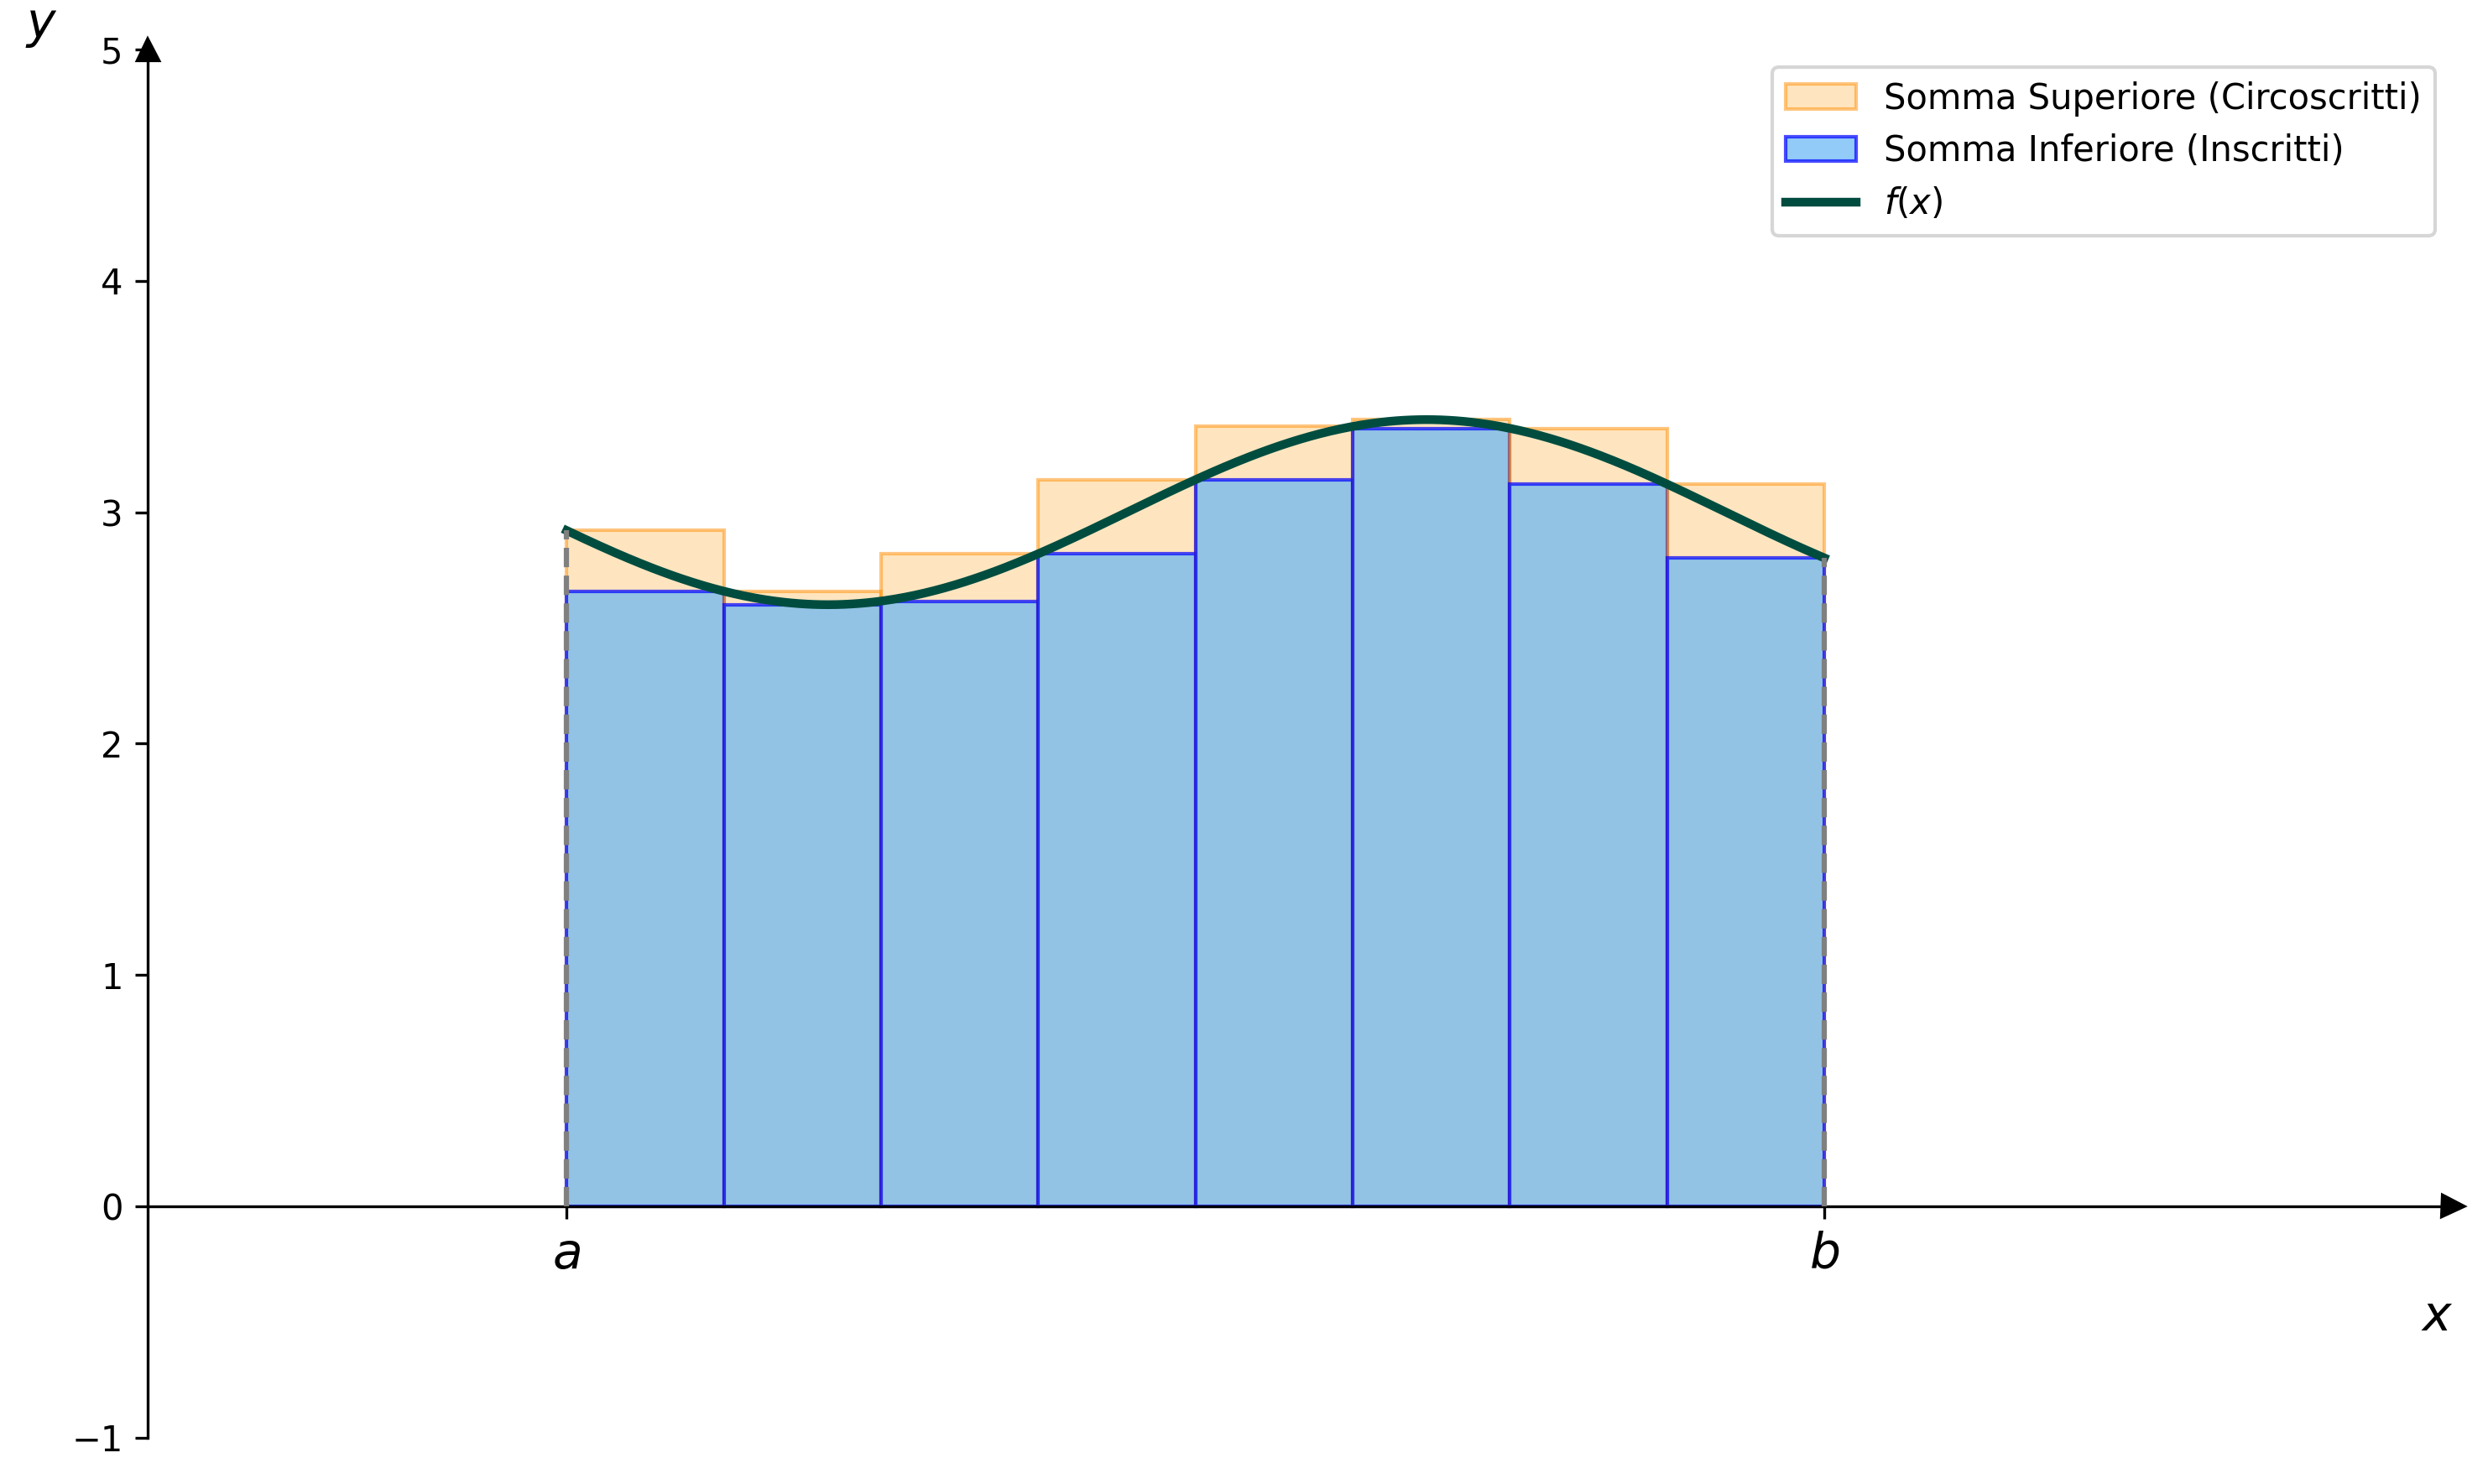
\includegraphics[width=0.8\textwidth]{img/stima_rettangoloide.png}
    \end{center}

\lem{}{
    Se $P \subseteq \overline{P}$ sono due partizioni di $[a,b]$ allora se $f: [a,b] \to \mathbb{R}$ è limitata, risulta che:
    \begin{align*}
    & s(P,f)\leq s(\overline{P},f)\\
    & S(P,f)\geq S(\overline{P},f)
    \end{align*}
}

\pf{
    Sia $P$ fissa, $P = \{ x_{0}=a , x_{1},x_{2},\dots, x_{n}=b \}$.

    Sia $\overline{P}= P \cup \{ z \}$.
    
    \begin{center}
    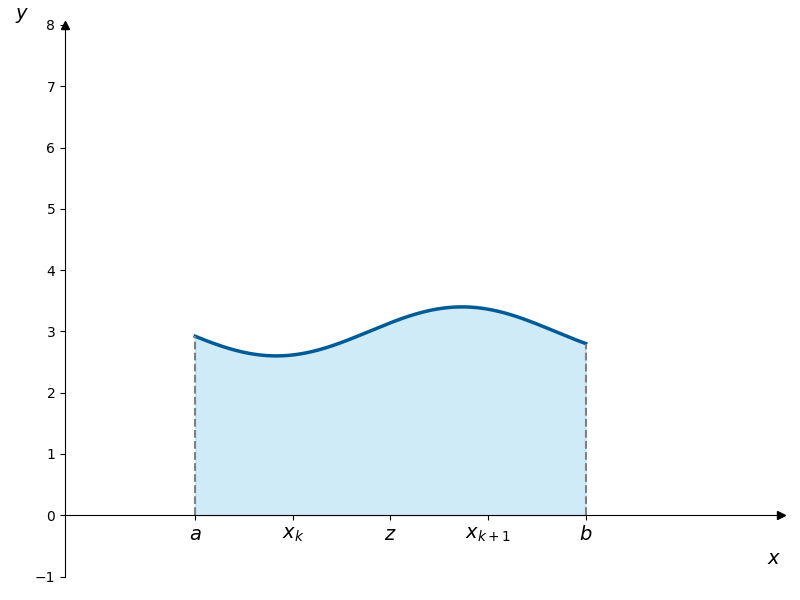
\includegraphics[width=0.8\textwidth]{img/rettangoloide_z.png}
    \end{center}


    \begin{align*} 
    & s(P,f)=m_{0}(x_{1}-a)+\dots+ \textcolor{orange}{m_{k}(x_{k+1}-x_{k})} +\dots+m_{n-1}(b-x_{n-1}) \\ 
    & s(\overline{P},f)= m_{0}(x_{1}-a)+\dots+\textcolor{orange}{m'_{k}(z -x_{k})+m''_{k}(x_{k+1}-z)}+\dots+m_{n-1}(b-x_{n-1}) 
    \end{align*}
    Dove:
    \[ m'_{k}=\inf_{[x_{k},z]}f\geq m_{k} \quad \text{e} \quad m''_{k}=\inf_{[z,x_{k+1}]}f\geq m_{k} \]
    Poiché $m'_k \ge m_k$ e $m''_k \ge m_k$ (l'inf su un insieme più piccolo è $\ge$ dell'inf sull'insieme grande), si ha:
    \begin{align*}
    &m'_{k}(z-x_{k})+m''_{k}(x_{k+1}-z)\geq m_{k}(z-x_{k}+x_{k+1}-z)\implies \\
    &m'_{k}(z-x_{k})+m''_{k}(x_{k+1}-z)\geq m_{k}(x_{k+1}-x_{k}) 
    \end{align*}
    Allora $s(P,f) \nearrow$. Allo stesso modo per $S(P,f)$.
}

\lem{Key-Lemma}{
    $\forall P, Q$ partizioni di $[a,b]$. Se $f:[a,b]\to \mathbb{R}$ è limitata, allora:
    \[ s(P,f)\leq S(Q,f) \]
        \begin{center}
    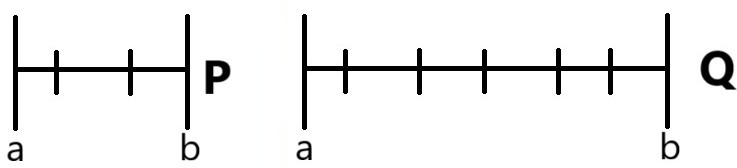
\includegraphics[width=0.8\textwidth]{img/key_lemma.jpg}
    \end{center}
}

\pf{
    Sia $R=P \cup Q$.
    \[ s(P,f)\le s(R,f)\leq S(R,f) \le S(Q,f) \]
}

\defn{Funzione integrabile secondo Riemann}{
    Definiamo:
    \[ A(f)=\{ S(P,f) , \quad P \text{ partizione} \} \]
    \[ B(f)=\{ s(P,f) , \quad P \text{ partizione} \} \]
    Allora $A(f)$ e $B(f)$ per il Key-Lemma sono separati, ovvero:
    \[ \inf A(f)=S(f)\geq \sup B(f)=s(f) \]
    Se sono contigui, ovvero $S(f)=s(f)=c$, allora diremo che $f$ è \textbf{integrabile} secondo Riemann.
    \[ c= \int_{\textcolor{magenta}{a}}^{\textcolor{magenta}{b}} \textcolor{blue}{f(x)} \, d\textcolor{orange}{x} \]
    e si chiama integrale definito.
    \[
    \begin{cases}
    \textcolor{magenta}{\text{Estremi di integrazione}}\\
    \textcolor{blue}{\text{Funzione integranda}}\\
    \textcolor{orange}{\text{Variabile d'integrazione}}
    \end{cases}
    \]
}

\subsection{Definizione con Limite}
Se voglio usare il limite:

\defn{Integrale definito con Limite}{
    Sia $P$ con passo $\frac{b-a}{n}$.
    \begin{align*}
    & s(P,f) \leq \frac{b-a}{n} \sum f(\overline{x}) \leq S(P,f) \quad \text{con } \overline{x}\in[x_{k},x_{k+1}]\\
    & \text{Le due quantità tendono rispettivamente a: } s(f) \text{ e } S(f)\\
    & \inf_{n}S(P_{n},f) = \sup_{n}s(P_{n},f)
    \end{align*}
}
    \begin{center}
    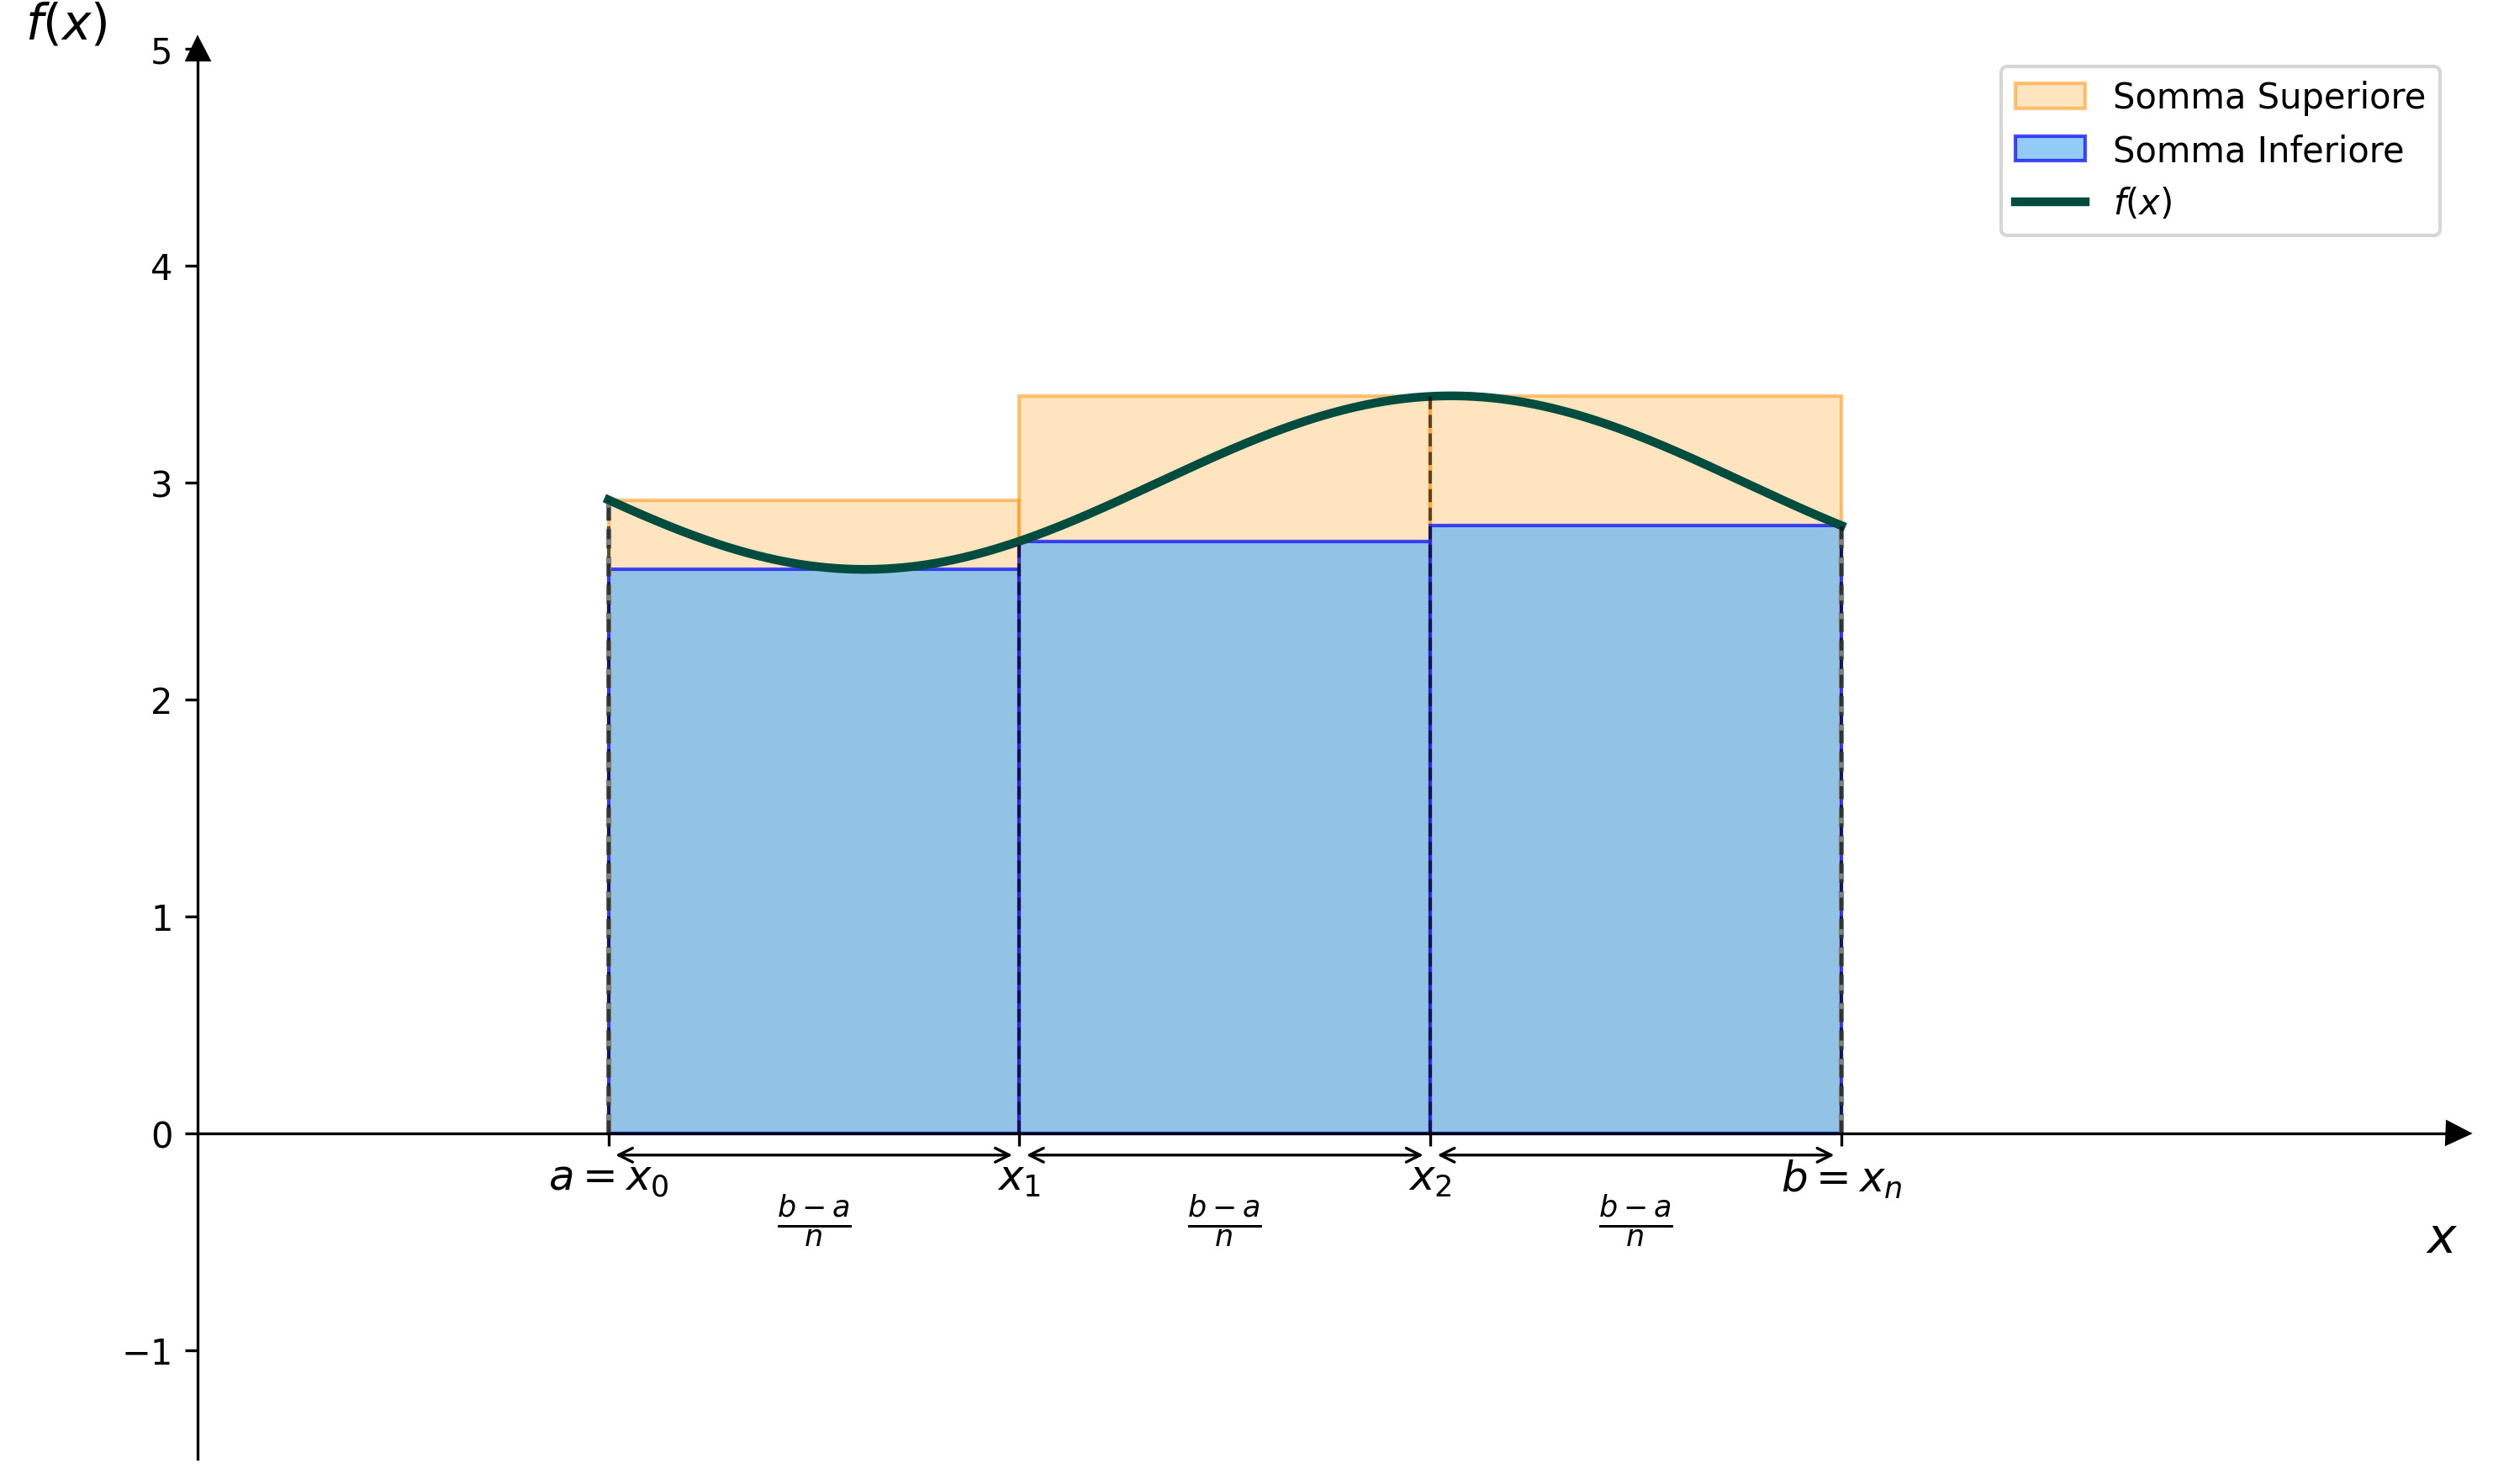
\includegraphics[width=0.8\textwidth]{img/stima_rettangoloide_n3.png}
    \end{center}

\ex{
    \textbf{Funzione di Dirichlet}: $f(x):[0,1]\to \{ 0,1 \}$
    \[
    f(x)=\begin{dcases}
    0 & x\in[0,1]\cap \mathbb{Q}\\
    1 & x\in[0,1]\setminus \mathbb{Q}
    \end{dcases}
    \]
    Considerando una partizione $P$:
    \begin{align*}
    &m_{k}= 0 \; \forall k \implies s(P,f)=0 \; \forall P\\
    &M_{k}= 1 \; \forall k \implies S(P,f)=\sum_{k=0}^{n} 1 \cdot (x_{k+1}-x_{k})=1  \; \forall P
    \end{align*}
}

\rmkb{
    Se $f\geq 0$ ed è integrabile in $[a,b]$ secondo Riemann, allora $\int_{a}^b f(x) \, dx$ geometricamente rappresenta l'area della porzione di piano compresa tra il grafico e l'asse $x$ che si chiama \textbf{Rettangoloide} relativo a $f$ di base $[a,b]$.
}

\rmkb{
    Se integro $f$ dispari in un intervallo simmetrico $[-a,a]$ allora:
    \[ \int^a_{-a} f(x) \, dx =0 \]
    Se $f$ è pari:
    \[ \int_{-a}^a f(x) \, dx =2\int_{0}^a f(x) \, dx \]
}

\subsection{Criterio di Integrabilità}
\prop{
    Sia $f$ limitata in $[a,b]$. $f$ è integrabile $\iff$ ($A(f),B(f)$ sono contigui) $\iff$
    $\forall \epsilon>0, \exists P \text{ partizione di } [a,b]:$
    \[ S(P,f)-s(P,f)<\epsilon \]
}

\subsection{Teorema Integrabilità delle funzioni continue}
\thm{Teorema Integrabilità delle funzioni continue}{
    Sia $f:[a,b]\to \mathbb{R}$ continua. Allora è integrabile secondo Riemann.
}

\pf{
    Per il Teorema di Heine-Cantor, $f$ è uniformemente continua.
    $\forall \epsilon>0, \exists \delta :$
    \[ |f(x')-f(x'')|<\epsilon \; \forall |x'-x''| < \delta \quad x', x'' \in [a,b] \]
    Sia $\epsilon$ fissato e sia $\delta$ il $\delta$ dell'uniforme continuità.
    Considero $P$ tale che $x_{k+1}-x_{k}$ è la stessa $\forall k$ e $x_{k+1}-x_{k}<\delta$.
    \[ S(P,f)-s(P,f)= \sum_{k=0}^{n} (M_{k}-m_{k})(x_{k+1}-x_{k})<\sum_{k=0}^{n} \epsilon(x_{k+1}-x_{k})=\epsilon(b-a) \]
}

\subsection{Teorema di Integrabilità delle Funzioni Monotone}
\thm{Teorema di Integrabilità delle Funzioni Monotone}{
    Sia $f$ monotona e $f:[a,b]\to \mathbb{R}$. Allora $f$ è integrabile secondo Riemann.
}

\pf{
    Immaginiamo $f$ crescente per fissare le idee. Si considera $P_{n}$ partizione di $n+1$ punti:
    \[ x_{k+1}-x_{k}=\frac{b-a}{n}\;\forall k = 0,\dots,n-1 \]
    \[ S(P_{n},f)= \sum_{k=0}^{n-1} M_{k}(x_{k+1}-x_{k})=\frac{b-a}{n} \sum_{k=0}^{n-1} M_{k} = \frac{b-a}{n}\sum_{k=0}^{n-1}f(x_{k+1}) \]
    \[ s(P_{n},f)=\frac{b-a}{n}\sum_{k=0}^{n-1} f(x_{k}) \]
    \begin{align*}
    & S(P_{n},f) - s(P_{n},f) = \frac{b-a}{n}\sum_{k=0}^{n-1} (f(x_{k+1})-f(x_{k})) \\
    & S(P_{n},f) - s(P_{n},f) = \frac{b-a}{n}(f(b)-f(a))
    \end{align*}
    Per il Criterio di Integrabilità, $f$ è integrabile.
}

\subsection{Proprietà degli integrali}
Siano $f,g: [a,b]\to \mathbb{R}$ integrabili. Allora:
\begin{enumerate}
    \item $f$ è integrabile in $[c,d]\subset [a,b]$.
    \item \textbf{Linearità}: $\int_{a}^b(\alpha f(x) +\beta g(x))\, dx = \alpha \int_{a}^b f(x) \, dx + \beta \int_{a}^b g(x) \, dx \quad \forall \alpha,\beta \in \mathbb{R}$.
    \item \textbf{Additività}: $\int_{a}^c f(x)\, dx + \int_{c}^b f(x) \, dx = \int_a^b f(x) \, dx \;\forall c \in ]a,b[$.
    \item Se $f(x)\leq g(x) \implies \int_{a}^b f(x) \, dx \leq \int_{a}^b g(x) \, dx$.
    \item Se $f(x)=k \quad \forall x \implies \int_{a}^b f(x) \, dx = k(b-a)$.
    \item Se $|f|$ è integrabile: $\left|\int_{a}^b f(x) \, dx\right|\leq \int_{a}^b |f(x)| \, dx$.
\end{enumerate}

\rmkb{
    Dalle proprietà 4 e 5, ottengo:
    \[ m (b-a) \leq \int_{a}^b f(x) \, dx \leq M (b-a) \]
    dove $m = \inf_{[a,b]} f$ e $M = \sup_{[a,b]} f$.
}

\subsection{Teorema della Media Integrale}
\prop{
    Sia $f: [a,b]\to \mathbb{R}$ continua. Allora $\exists c \in [a,b]:$
    \[ \int_{a}^b f(x) \, dx = f(c)(b-a) \]
}

\pf{
    Poniamo $y= \frac{\int_{a}^b f(x) \, dx}{b-a}$.
    Per le proprietà precedenti:
    \[ m\leq \frac{\int_{a}^b f(x) \, dx}{b-a} \leq M \]
    con $m=\min_{[a,b]}f$ e $M = \max_{[a,b]}f$ (poiché continua).
    Per il Teorema dei valori intermedi: $\exists c: y = f(c)$.
}

\subsection{Funzione Integrale}
\defn{Definizione}{
    Sia $f$ integrabile in $[a,b]$ e sia $x_{0}\in[a,b]$. Allora $\forall x \in [a,b]$ posso definire:
    \[ F(x)=\int_{x_{0}}^x  f(t) \, dt \]
    che si chiama \textbf{funzione integrale} relativa a $f$ di punto iniziale $x_{0}$.
}

\thm{Teorema Fondamentale del Calcolo Integrale}{
    Sia $f:[a,b]\to \mathbb{R}$ continua. Sia $x_{0}\in[a,b]$.
    Allora la funzione integrale $F(x)= \int_{x_{0}}^x f(t) \, dt$ è derivabile e risulta:
    \[ F'(x)=f(x) \quad \forall x \in [a,b] \]
}

\pf{
    Tesi: $\lim_{ h \to 0 } \frac{F(x+h)-F(x)}{h}= f(x)$.
    \begin{align*}
    \lim_{ h \to 0 } \frac{\int_{x_{0}}^{x+h} f(t) \, dt - \int_{x_{0}}^x f(t) \, dt}{h} &= \lim_{ h \to 0 } \frac{\int_{x_{0}}^{x+h} f(t) \, dt + \int_{x}^{x_{0}} f(t) \, dt}{h}\\
    &= \lim_{ h \to 0 } \frac{1}{h} \int_{x}^{x+h}f(t)\, dt \\
    &= \lim_{ h \to 0 } \frac{1}{ h } \cdot f(c_{h}) \cdot {h} \quad (\text{dove } c_{h} \in [x, x+h])\\
    &= f(x)
    \end{align*}
    L'ultimo passaggio vale per la continuità di $f$ (se $h\to 0$, $c_h \to x$).
}

\rmkb{
    \textbf{Formula Fondamentale del Calcolo Integrale}: Fissato $x_{0}=a$,
    \[ \int_{a}^b f(t) \, dt =F(b)-F(a) \]
}

\section{Integrazione Indefinita}
\defn{Primitiva}{
    Sia $f: [a,b] \to \mathbb{R}$. Si chiama \textbf{primitiva} di $f$ una funzione $F$ derivabile in $[a,b]$ tale che:
    \[ F'(x) = f(x) \quad \forall x \in [a,b] \]
}

\thm{Caratterizzazione delle primitive in un intervallo}{
    Sia $f: [a,b] \to \mathbb{R}$ continua. Se $F(x)$ e $G(x)$ sono due primitive di $f$, allora esse differiscono per una costante:
    \[ \exists c \in \mathbb{R}: G(x) = F(x) + c \]
}

\defn{Integrale Indefinito}{
    Sia $f$ continua in $[a,b]$. L'insieme di tutte le primitive si indica con $\int f(x) \, dx$ e si chiama \textbf{integrale indefinito}.
    \[ \int f(x) \, dx = F(x) + c \]
}



\section{Funzioni Sommabili}

\ex{
    \textbf{Funzioni "problematiche"}
    \[ \frac{1}{x^\alpha} \quad \text{in } ]0,1] \implies \int_{0}^1 \frac{1}{x^\alpha} \, dx = \,? \]
    \[ \frac{1}{x^\alpha} \quad \text{in } [1,+\infty[ \implies \int_{1}^{+\infty} \frac{1}{x^\alpha} \, dx = \,? \]
}

\defn{Funzione Sommabile}{
    Sia $f\geq 0$ in $[a,b[\:(b\in \mathbb{R}, b =+\infty)$ oppure in $]a,b] \; (a\in \mathbb{R}, a= -\infty)$.
    Supponiamo che $f$ sia integrabile in ogni sottointervallo di $]a,b]$ oppure di $[a,b[$.
    \[ \textcolor{orange}{\forall x \in [a,b[ \quad F(x)= \int_{a}^x \underbrace{{ f(t) }}_{\geq 0} \, dt \quad \nearrow } \]
    \[ \exists \lim_{ x \to b^- } \int_{a}^x f(t)\, dt = \begin{cases}
    +\infty \\
    l \in \mathbb{R}^+
    \end{cases} \]
    Se il \textbf{limite} $\exists$ \textbf{finito}, diremo che $f$ è \textbf{sommabile} in $[a,b[$ e
    \[ \int_{a}^b f(x) \, dx = \lim_{ x \to b^- } \int_{a}^x f(t) \, dt \]
    Discorso analogo per $a$:
    \[ \int_{a}^b f(x)\, dx = \lim_{ x \to a^+ }\int_{x}^b f(t) \, dt \quad \text{ se } \exists \text{ finito} \]
    Se il \textbf{limite non è finito}, $f$ \textbf{non è sommabile}.
}

\ex{
    $\displaystyle \frac{1}{x^\alpha} \; \text{in } ]0,1] \text{ è sommabile?}$
    
    Pongo $\alpha>0$ così che stia al denominatore.
    \[ \int_{x}^1 \frac{1}{t^\alpha} \, dt = \begin{dcases}
    \alpha=1 \implies \log t\Big|^1_{x} = - \log x \\
    \alpha \neq 1, \,\alpha>0 \implies \frac{t^{-\alpha+1}}{-\alpha+1}\Bigg|^1_{x}=\frac{1}{1-\alpha}- \frac{x^{1-\alpha}}{1-\alpha}
    \end{dcases} \]
    \[ \lim_{ x \to 0^+ } \int_{x}^1 \frac{1}{t^\alpha} \, dt = \begin{dcases}
    \alpha=1 \implies l=+\infty \implies f \text{ non è sommabile} \\
    1-\alpha<0 \implies l=+\infty \implies f \text{ non è sommabile} \\
    1-\alpha>0 \implies l=\frac{1}{1-\alpha} \implies f \text{ è sommabile}
    \end{dcases} \]
    \[ \frac{1}{x^\alpha} \text{ in } ]0,1] \text{ è \textbf{sommabile}} \iff 0\leq\alpha<1 \]
}

\ex{
    $\displaystyle \frac{1}{x^\alpha} \; \text{in } [1,+\infty[ \text{ è sommabile?}$
    
    \[ \lim_{ x \to +\infty } \int_{1}^x \frac{1}{t^\alpha}\, dt = \begin{dcases}
    \alpha=1 \implies \log x \overset{x \to +\infty}{\to}l=+\infty \implies \text{non è sommabile} \\
    \alpha\neq 1 \implies \frac{x^{1-\alpha}}{1-\alpha} - \frac{1}{1-\alpha}\implies \text{è sommabile } \iff 1 -\alpha <0 \implies \alpha>1
    \end{dcases} \]
}

\subsection{Criteri per le Funzioni Sommabili}

\prop{Criterio del Confronto}{
    Se $0\leq f(x)\leq g(x)$ definite nello stesso insieme e $g$ sommabile $\implies f$ è sommabile.
}

\pf{
    La dimostrazione è ovvia (segue dal Teorema del Confronto Integrale).
}

\prop{Criterio degli Infinitesimi}{
    Sia $f\geq 0$ continua in $[a,+\infty[$.
    Se $\displaystyle \lim_{ x \to +\infty } x^\alpha f(x)= l> 0 \, ,l\in \mathbb{R} \implies \begin{cases}
    \alpha>1 \implies f \text{ è sommabile} \\
    \alpha \leq 1 \implies f \text{ non è sommabile}
    \end{cases}$
}

\pf{
    Applichiamo la definizione di limite. Sia $\epsilon=\frac{l}{2}$.
    \[ \exists M>0: \forall x > M \quad \frac{l}{2} = l-\epsilon < x^\alpha f(x) < l + \epsilon = \frac{3}{2} l \]
    Implica che $\forall x > M$:
    \[ f(x)< \frac{3}{2}l \cdot\frac{1}{x^\alpha} \quad \text{SOMMABILE (per confronto con } \frac{1}{x^\alpha}, \alpha > 1 \text{)} \]
    \[ f(x)> \frac{l}{2} \cdot\frac{1}{x^\alpha} \quad \text{NON SOMMABILE (per confronto con } \frac{1}{x^\alpha}, \alpha \le 1 \text{)} \]
}

\rmkb{
    \textbf{Criterio degli Infiniti}: Lo stesso Criterio vale all'infinito all'inversione delle condizioni.
}

\subsection{Relazione tra Serie e Integrali}

\ex{
    Consideriamo $\frac{1}{n}$.
    \begin{align*}
    & \int_{n}^{n+1} \frac{1}{x} \, dx \leq \frac{1}{n}\\
    & \frac{1}{n} = \int_{n}^{n+1} \frac{1}{n} \, dx = \frac{1}{n}(n+1-n)\\
    & a_{n} \geq 0\\
    & a_{n} = \int_{n}^{n+1} a_{n} \, dx \\
    & \sum_{n=1}^{+\infty} \int_{n}^{n+1} \frac{1}{x} \, dx \leq \sum_{n=1}^{+\infty} \frac{1}{n}\\
    & \int_{1}^{+\infty} \frac{1}{x} \, dx \leq \sum_{n=1}^{+\infty} \frac{1}{n}\\
    & \text{Dato che } \frac{1}{x} \text{ non è sommabile, } \sum_{n=1}^{+\infty} \frac{1}{n} \text{ diverge.}
    \end{align*}
}

\rmkb{
    Vale questo confronto anche per:
    \[ \sum_{n=1}^{+\infty} \int_{n}^{n+1} \frac{1}{x^\alpha} \, dx \leq \sum_{n=1}^{+\infty} \frac{1}{n^\alpha} \]
}

\thm{Criterio Integrale per le Serie}{
    Sia $f\geq 0$ e decrescente ($\searrow$) e sia $|a_{n}| \leq f(n)$.
    Se $f$ è sommabile in $[1,+\infty[ \implies \sum a_{n}$ converge.
}

\end{document}
